\documentclass[12pt,a4paper]{report}
\usepackage[english]{babel}
\usepackage[T1]{fontenc}
\usepackage{times}
\usepackage{amsmath}
\usepackage{amsfonts}
\usepackage{amssymb}
\usepackage{textcomp}
\usepackage{gensymb}
\usepackage{hyperref}
\usepackage{graphicx}
\usepackage{setspace}
\usepackage[version=4]{mhchem}
\usepackage{caption}
\usepackage{subcaption}
\usepackage{longtable}
\usepackage{multirow}
\usepackage[dvipsnames]{xcolor}
\usepackage{tikz}
\usepackage{wrapfig}
\usepackage[left=2cm,right=2cm,top=2cm,bottom=2cm]{geometry}
\title{Interpolation of component characteristic maps for thermodynamic cycle assessment}
\author{Martin Heylen}
\newcommand{\citep}[1]{\cite{#1}}
\newcommand{\vect}[1]{\boldsymbol{#1}}

\begin{document}
\makeatletter
\newenvironment{folding}{\endgroup}{\begingroup \def \@currenvir{folding}\edef \@currenvline{\on@line}}
\makeatother
\maketitle

\tableofcontents
\listoffigures
\listoftables
%%%%%%%%%%%%%%%%%%
%% Chapter 1:   %%
%% Introduction %%
%%%%%%%%%%%%%%%%%%
%\input{Chapter1_introduction}
\setstretch{1.5}
\chapter{Introduction}

\newpage
%%%%%%%%%%%%%%%%%%%%%%%%%%%%%%%%%
%% Chapitre 2:                 %%
%% Notion of thermodynamics    %%
%%%%%%%%%%%%%%%%%%%%%%%%%%%%%%%%%
\graphicspath{{Chapitre_2/Images/}}
\chapter{Notions of thermodynamics}\label{C2}
%%%%%%%%%%%%%%%%%%%%%%%%%%%%%%%%%%%
%%%%%                         %%%%%
%%%%% Introduction chapitre 2 %%%%%
%%%%%                         %%%%%
%%%%%%%%%%%%%%%%%%%%%%%%%%%%%%%%%%%
\quad\, The principle and uses of the Brayton cycle have been discussed in the introduction. As explained, this concept has been applied for many usages, including electricity production and aircraft propulsion which are the most common and known applications. It has been exposed that from the invention proposed by George Brayton in the end of the 19th century, the technology did really evolve.

Indeed, while the Brayton cycle engine first appears as a  piston engine where the compression, combustion and expansion occurs in the same enclosure, Nowadays 
the process is shared between at least three components (namely the compressor, the turbine and the combustion chamber).

However, the keys notions to understand how theses components behave have not been introduced yet. This problematic will be covered by this chapter, which will introduce step-by-step those notions.

\section{Fundamental notions}
%%%%%%%%%%%%%%%%%%%%%%%%%%%%%%%%%%%
%%%%%                         %%%%%
%%%%% <<Fundamental notions>> %%%%%
%%%%%                         %%%%%
%%%%%%%%%%%%%%%%%%%%%%%%%%%%%%%%%%%
\quad\, As mention in the lead-in of this chapter, the first sections of this report will entirely be devoted to the bringing in of the required knowledge for the understanding of the full report.

Starting from very fundamental notions, those will allow to explain more complex concept that will be applied in this work.

\subsection{Open/closed system}\label{sect:C2_Sys}
\quad\,  The thermodynamic is a science that "studies the exchange of energy between a system and its environment or surrounding" \cite{thermoApp_1}.

The system is defined as being the area of the space selected for the study. Between the system and the environment lies the boundary. This boundary can either be real or fictitious and, can be static or mobile.

When the system is characterized, it has to be established if it is an open or a closed system.
The open systems are ones where an arbitrary control volume well demarcated in the space is studied. In contrast to closed systems, open systems not only exchange work and heat with the environment, but also matter. Typical examples are combustion chamber, heat-exchanger, turbomachines, piping,...

On the other hand, the closed systems does not exchange matter with the environment. Indeed, 
for those systems a control mass well delimited in the space is studied. Therefore, the exchange of mass with the environment is prohibited for this category of system. 

\subsection{State functions and variables}\label{sect:C2_State}
\quad\, Let considered a system as defined in the previous section. The state functions are defined as "a property of the system that only depend on its current state". These functions are independent of the past of the system and describe the equilibrium state of the system.

When the state functions can be measured (directly or indirectly), these are called state variables. For example, the pressure $p$, the temperature $T$ or the volume $Vol$ are state variables.


In this work, the units used for the state and function variables follows the international system (SI) of units \cite{Nist}. 
\subsubsection{Pressure}
\quad\, The pressure unit is the Pascal (Pa). 1 Pa corresponds to 1 N/m$^2$, where 1 N (kg$\cdot$m/s$^2$) is the required force to increase each second by 1m/s the velocity of a body weighting 1kg.

The pressure is also often expressed in bar, unit corresponding to 1e5 Pa.

\subsubsection{Temperature}
\quad\, The temperature unit is the degree Kelvin (K). 273.15\degree K corresponds to 0\degree C, temperature at which pure water starts freezing.

\subsubsection{Volume}
\quad\, The volume unit is the meter cube (m$^3$).

\subsection{Ideal gas equation}
\quad\, It can be shown that the equilibrium state of a system can be described by those three variables. Also, among $P$, $T$ and $Vol$, only two of them are independent. This means that a state relation defined as \textbf{F}($P$, $T$, $Vol$) = 0.

For the ideal gas, this relation is
\begin{align}
\setstretch{1}
p\cdot Vol &= m\cdot\frac{R}{MM}\cdot T\nonumber\\
p\cdot vol &= r\cdot T\label{eq:C2_GP}    
\end{align}
where \textit{m} is the quantity of matter (in kg), $R$ is the universal gas constant (8.314 J/mole/K), $vol$ the specific volume (in m$^3$/kg) and $MM$ is the molar mass (in kg/mole\footnote{Where 1 mole correspond to $\sim 6\cdot 10^{23}$ elementary entities (atoms, molecules,...)}) of the system. The density $\rho$ of the gas is given as being one o

\subsection{Energy}\label{sect:C2_Ener}
\quad\, In the subsection \ref{sect:C2_Sys}, the notion of energy has been mentioned without characterizing it before hand. From the first principle of the thermodynamic, it is stated that the energy cannot be created nor destroyed. Therefore, it can only be converted an can exist into multiple forms (thermal, mechanical, electrical,...)\cite{thermoApp_2}. 

The unit of the energy is the Joule (J), and the sum of all the energies in a system is called the total energy $E$. 1J is the work to move a body over 1 meter using a force of 1N.\\


The energy is a state variable. This means that this quantity allows to characterize the state of the system. When considering the energy, its absolute value is not something that is defined. Instead, the energy is always computed as compared with a reference point.

Thus, considering the variation of the total energy from a state \textbf{1} to a state \textbf{2}, it is obtained

\begin{equation}
\setstretch{1}
    \Delta E = \Delta U + \Delta KE + \Delta PE \label{eq:C2_E}
\end{equation}

\begin{align*}
\setstretch{1}
    \text{with } \Delta U  &= U_2 - U_1 =  m\cdot(u_2 - u_1) \text{: Variation of the internal energy}\\
                 \Delta KE &= \frac{1}{2}m\cdot(v^2_2 - v^2_1)\text{: Variation of the kinetic energy}\\
                 \Delta PE &= m\cdot g\cdot(z_2 - z_1)\text{: Variation of the potential energy}
\end{align*} 

where $z$ is the altitude of the system position (m), $v$ is the velocity of the fluid (m/s) and $U$, the internal energy, is the sum of all the "microscopic" energy within the system (J). $u$ corresponds to the specific internal energy, and its unit is in J/kg.

As said in the subsection \ref{sect:C2_Sys}, any system will exchange energy with the surrounding as heat and/or work. The heat is defined as "the form of energy which is exchanged between the system and its environment when there is a gradient of temperature between these two entities". As the heat is always referred as a flux between two bodies, the phenomena is called heat transfer. The heat transfer can be realized by
\begin{itemize}
\setstretch{1}
    \item Conduction: Heat transfer through a non flowing material due to the interaction of "molecular scale energy carriers within the material"\cite{GregoryNellis2015}
    \item Convection: More complex conduction when considering a flowing fluid.
    \item Radiation: The heat is transferred as electromagnetic waves.
\end{itemize}
The heat transfer is denoted $Q$. A system that does not exchange heat with the surrounding is called \textbf{adiabatic}.

Aside the heat transfer, the system also can exchange energy by producing a work. The Work $W$ is "the form of energy exchanged associated to a force applied over a certain distance". The work is exchanged if the force applied on the system creates a displacement of its boundary. The power is defined as the work per unit of time (in Watt or W).

Both the heat and the work are called "path functions" because they are associated to the evolution of a system and not to the state of this system. Thus, these are not thermodynamic variables (like the temperature or the pressure).

\subsubsection{Energy balance}
\quad\, It has been previously mentioned several mechanisms to exchange energy from the system to its environment. Aside from the heat transfer and the work transfer, the energy can also be exchange using mass transfer. Indeed, if the considered system is open, the mass entering and exiting the system will convey energy.

To recall the first principle of the thermodynamic, the energy cannot be created or destroyed. Based on the statement, the energy balance of the system is given by the following generic formulation (\ref{eq:C2_EB}).
\begin{equation}
\setstretch{1}
    E_{in} - E_{out} = (Q_{in} - Q_{out}) + (W_{in} - W_{out}) + (E_{mass,in} - E_{mass,out}) = \Delta E_{system} \label{eq:C2_EB}
\end{equation}
with $E_{mass}$ the energy convey by the mass entering/exiting the system.

It is possible to write a temporal formulation (\ref{eq:C2_PB}) of the energy balance named \textbf{power balance}.  
\begin{equation}
\setstretch{1}
    \dot{E}_{in} - \dot{E}_{out} = (\dot{Q}_{in} - \dot{Q}_{out}) + (\dot{W}_{in} - \dot{W}_{out}) + (\dot{E}_{mass,in} - \dot{E}_{mass,out}) = \frac{dE_{system}}{dt} \label{eq:C2_PB}
\end{equation}
where $\frac{dE_{system}}{dt}=0$ when considering a system for which the variation of energy does not vary in the time.

\subsubsection{Energy conservation efficiency}
\quad\, When the system is transferring or converting energy, it is often interesting to quantified the quality of this transfer/conversion. the efficiency is defined to provide this quantification and its definition is the
$\frac{\text{Desired ouptut}}{\text{Required input}}$. For example, a water electric heater with a efficiency of 90\% is a system such that 90\% of the electrical energy consumed is converted in thermal energy.  

Considering the combustion of a fuel, the combustion efficiency is defined as the ratio
$$ \frac{\dot{Q}}{\dot{m}_{fuel}\cdot HV_{fuel}}$$
where $\dot{m}$  and $HV_{fuel}$ is the mass flow and the heating value of the fuel injected into the combustion chamber.
\section{Principles of thermodynamic}
%%%%%%%%%%%%%%%%%%%%%%%%%%%%%%%%%%%
%%%%%                         %%%%%
%%%%% <<Principle of thermo>> %%%%%
%%%%%                         %%%%%
%%%%%%%%%%%%%%%%%%%%%%%%%%%%%%%%%%%

\quad\, The previous section did introduce many concepts to start analyzing a thermodynamic system submitted to diverse transformations. Among those, the notion of state variables defining the equilibrium state of such system has been defined. This section will used the first and second principles of the thermodynamic to introduce some state variables that are used when studying a thermodynamic cycle.

\subsection{Enthalpy}
\quad\, Considering a closed system, the third term of the energy balance given in the relation(\ref{eq:C2_EB}) is nullified. Thus, the variation of the total energy from a state \textbf{1} to a state \textbf{2} is equal to
\begin{equation}
\setstretch{1}
E_{2} - E_{1} = Q_{1-2} - W_{1-2} = m\cdot\left(u_2 - u_1\right) + \frac{1}{2}m\cdot\left(v^2_2 - v^2_1\right) + m\cdot g\cdot\left(z_2 - z1\right)\citep{Dewallef2019} \label{eq:C2_EBC}
\end{equation}
Let's note that the terms of kinetic and potential energy are often negligible compared to the internal energy.  

The relation \ref{eq:C2_EBC} can be adapted to be applied for the open system by introducing an accumulation term $\Delta E_{cv}$. This correction allows the following reformulation (\ref{eq:C2_EBO}) of the energy balance.
\begin{equation}
\setstretch{1}
Q_{1-2} - W_{1-2} - E_{2} - E_{1} = \Delta E_{cv}\label{eq:C2_EBO}
\end{equation}

\begin{figure}[h]
\centering
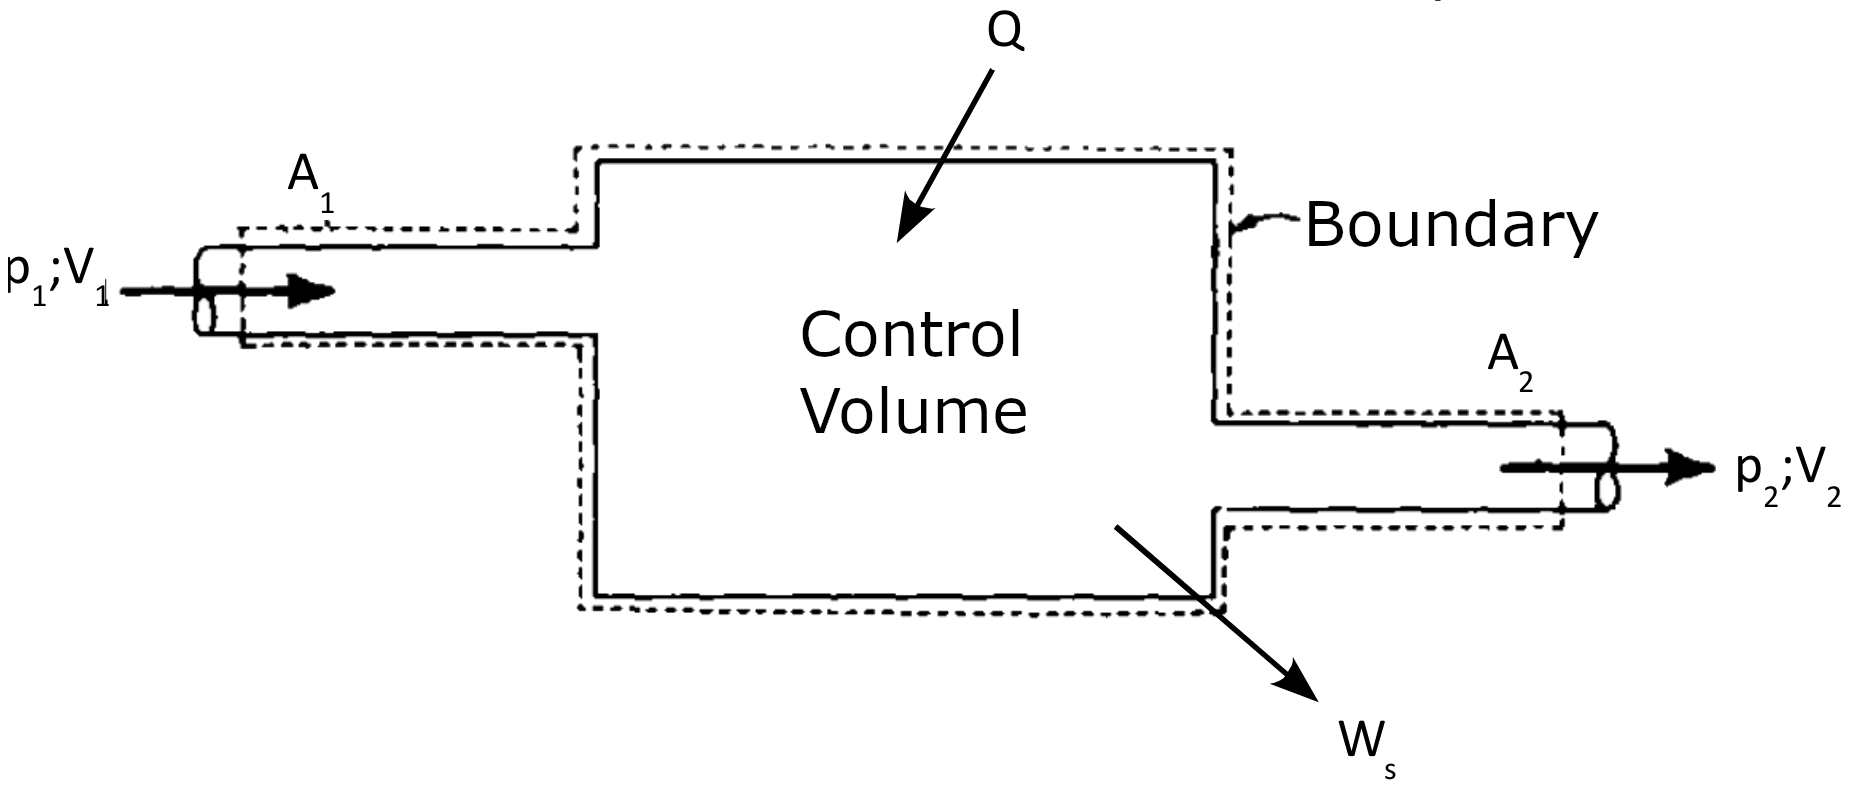
\includegraphics[width=0.7\textwidth]{control_volume.png}
\caption{System control volume \cite{Dewallef2019}}
\label{fig:C2_VC}
\end{figure}

The Figure \ref{fig:C2_VC} depicts an open system with an entry and exit area $A_1$ and $A_2$ respectively. Posing that the work $W$ is equal to 
\begin{equation}
\setstretch{1}
W = p_2\cdot A_2\cdot v_2\cdot \Delta t - p_1\cdot A_1\cdot v_1\cdot \Delta t + W_s
\end{equation}      
where $P_1$ (resp. $P_2$) and $V_1$ (resp. $V_2$) are the pressure and the velocity at \textbf{1} (resp. \textbf{2}).

By neglecting the variation of the kinetic and potential energy, the energy balance is after some mathematical operations as given in the relation \ref{eq:C2_EBH}
\begin{equation}
\setstretch{1}
q - w_s = u_2 +p_2\cdot vol_2 - u_1 - p_1\cdot vol_1 = h_2 - h_1\label{eq:C2_EBH}
\end{equation}
where $q$, $w_s$, and $h$ are respectively the specific work, heat and \textbf{enthalpy} (in J/kg).  
For the case of an ideal gas, the enthalpy and the internal energy only depend on the temperature $T$. Indeed, taking the equation (\ref{eq:C2_GP}), the relation (\ref{eq:C2_h}) can easily be deduced.
\begin{equation}
\setstretch{1}
h = u(T) + p\cdot vol = u(T) + r\cdot T \label{eq:C2_h}
\end{equation}
\subsection{Specific heat}
\quad\, The previous subsection was meant to define the enthalpy. This state variable is used in place of the internal energy when dealing with open system.\\

An other quantity that is useful for system study is the \textbf{specific heat}. This state variable is defined as the required energy to increase of 1\degree C the temperature of 1kg of a substance. 
 
The required heat to produce this effect depends on the ways the transformation takes place. 
If it is done under constant volume constraint, it is called specific heat at constant volume and denoted $c_v$. 

If the transformation is performed at constant pressure, the symbol associated to the specific heat is $c_p$.
It is worth to note that the specific heat at constant pressure is always higher than the $c_v$. When performing the transformation a constant pressure, the gas expands against the external pressure. This means that the gas does work and, this is the reason behind the greater value of the supplied heat when dealing with a transformation at constant pressure. 

It had been shown that for an ideal gas, the variation of the internal energy can be linked to the specific heat at constant volume as written in the relation (\ref{eq:C2_UC}).
\begin{equation}
\setstretch{1}
du = c_vdT \rightarrow u_2 - u_1 = \int_{T_1}^{T_2} c_vdT\label{eq:C2_UC}
\end{equation} 
Similarly, the variation of the enthalpy can be expressed using the specific at constant pressure.

\begin{equation}
\setstretch{1}
dh = c_pdT \rightarrow h_2 - h_1 = \int_{T_1}^{T_2} c_pdT\label{eq:C2_UP}
\end{equation} 

These two relations, with the equality (\ref{eq:C2_h}), provide the required tools to express the gas constant $r$ as a function of the temperature only. 
\begin{equation}
\setstretch{1}
r = c_p - c_v \label{eq:C2_r}
\end{equation}

Aside the gas constant, the specific heat ratio $k$ (\ref{eq:C2_k}) is also a useful variable to be computed.
\begin{equation}
\setstretch{1}
k = \frac{c_p}{c_v} \label{eq:C2_k}
\end{equation}
\subsection{Carnot cycle}
\quad\, The previous subsections used the first principle of the thermodynamic to deduce two useful state variables, namely the enthalpy and the specific heat.

Now, let's move aside those notions and let consider the case where the transformation applied to a system is reversible. A necessary condition for the reversibility is that the transformation has to be done in quasi-equilibrium. This implies that if the transformation is reversed, the system goes back to its initial state.


\begin{figure}[h]
\centering
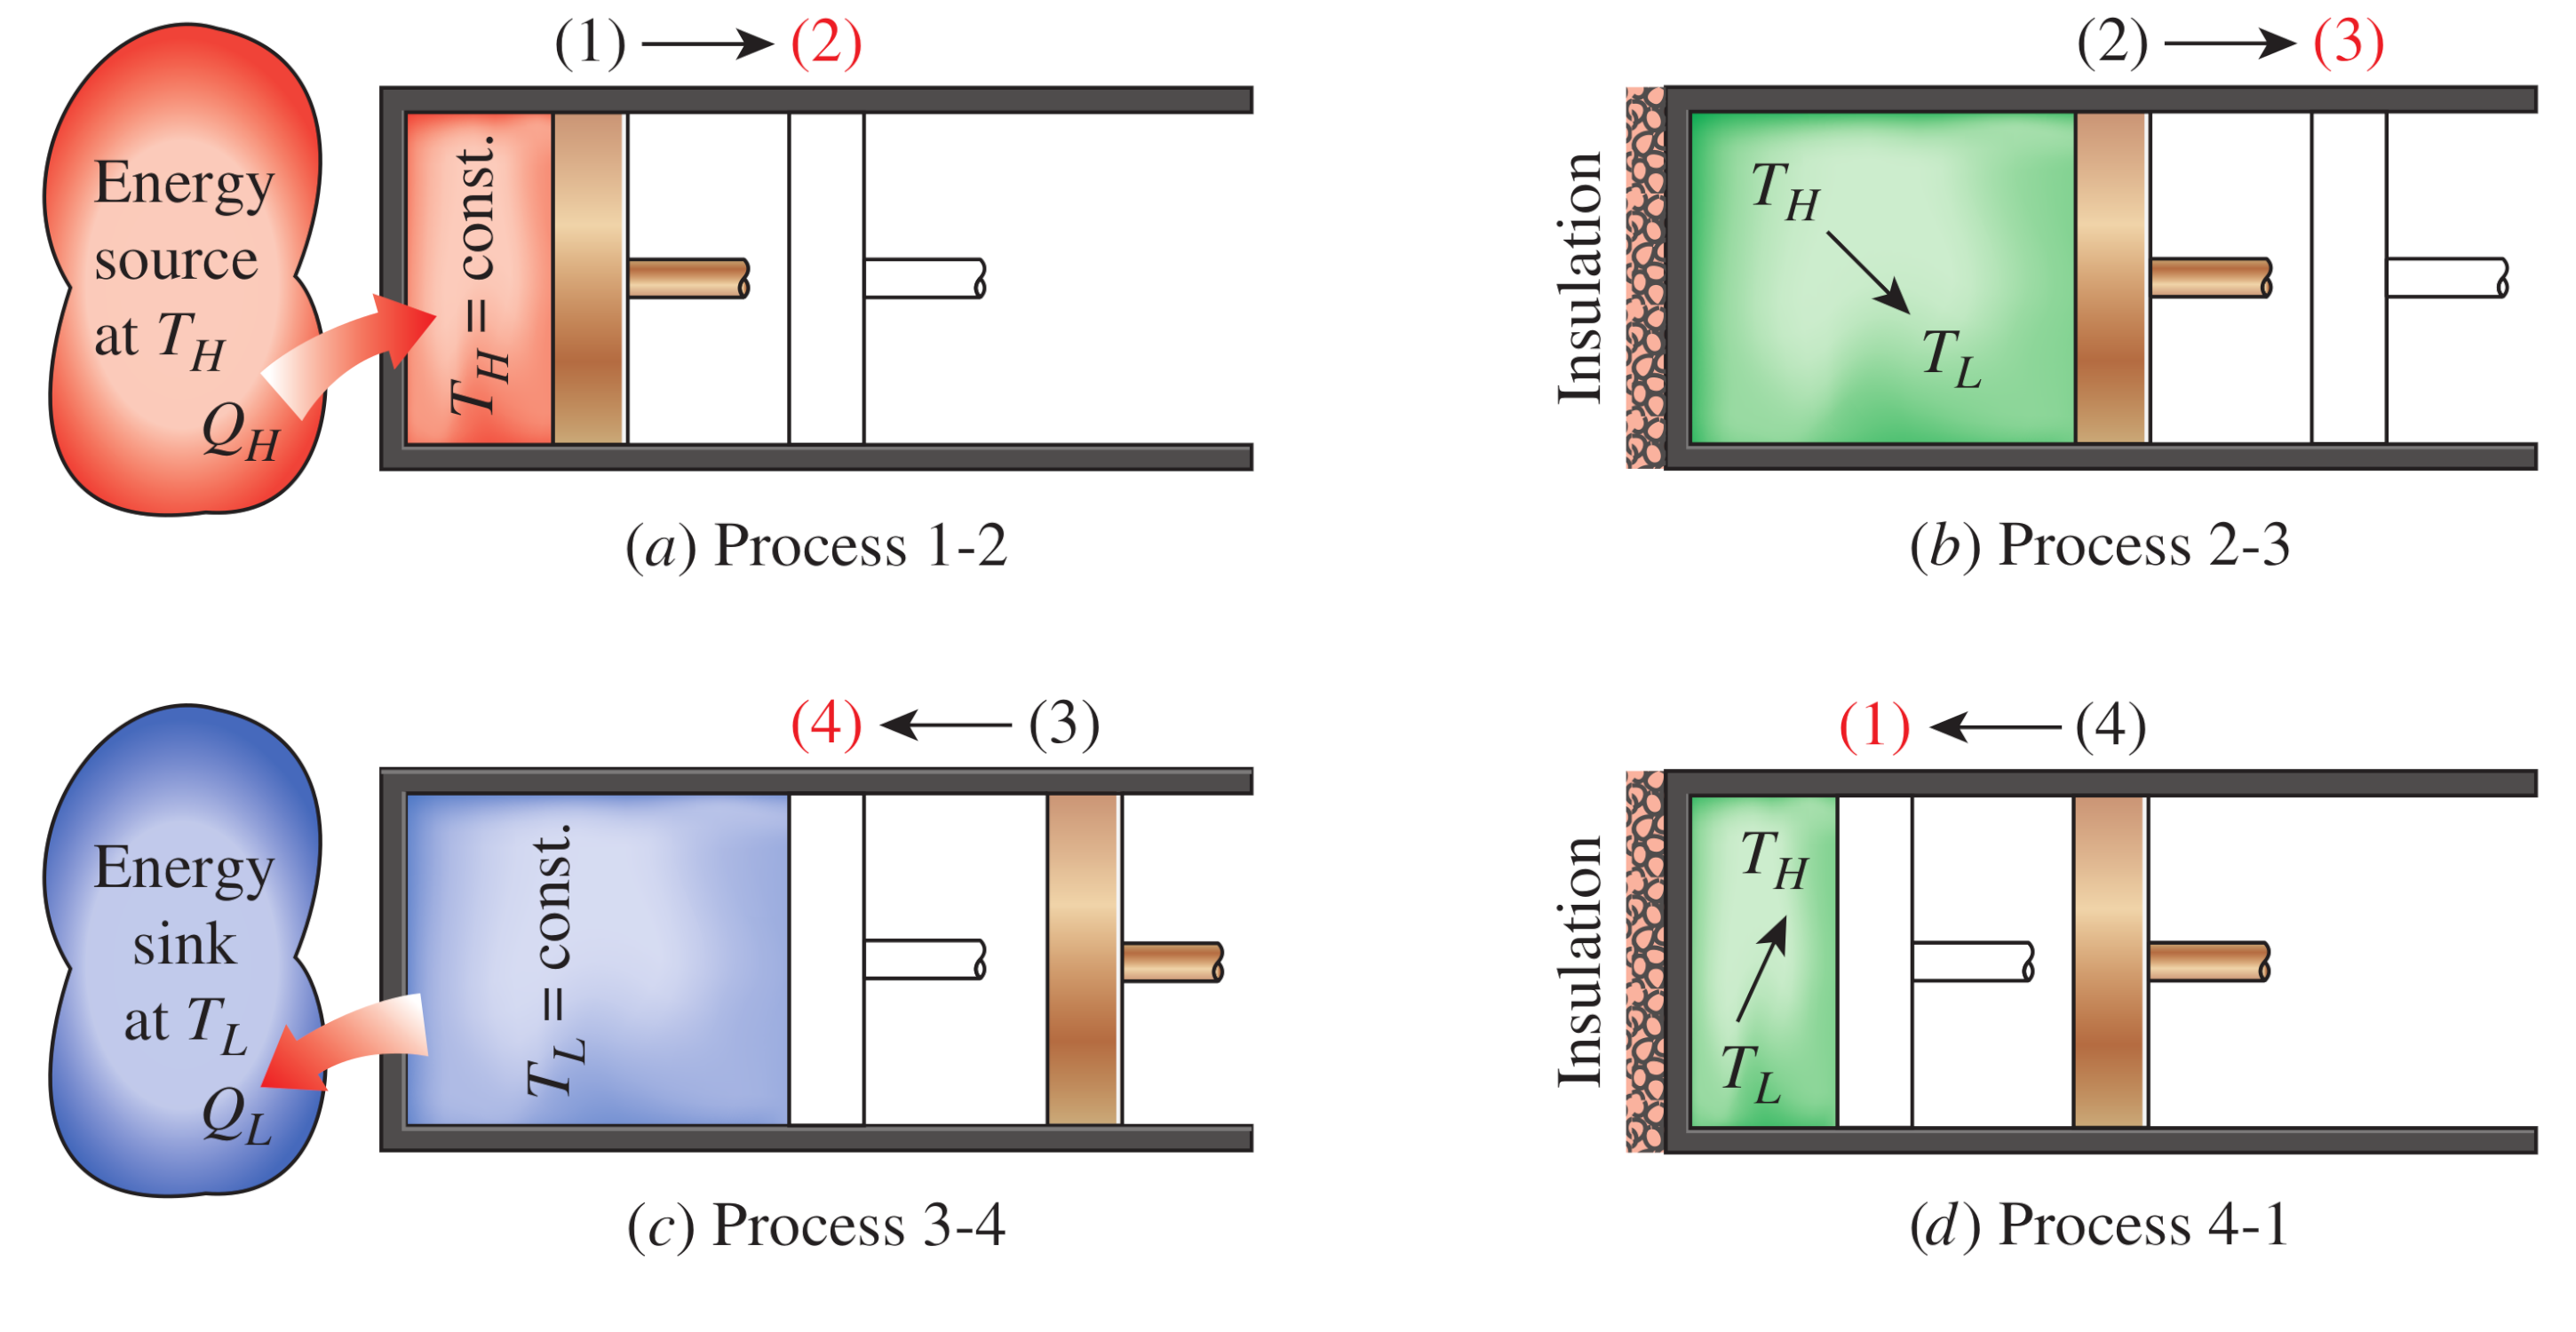
\includegraphics[width=0.7\textwidth]{Carnot_schema.png}
\caption{Carnot cycle - Schematic \cite{2015}}
\label{fig:C2_Carnot}
\end{figure}
The Carnot cycle is a thermodynamic cycle composed of 4 reversible transformations illustrated on Figure \ref{fig:C2_Carnot}. The transformations are defined as follows.

\begin{itemize}
\setstretch{1}
\item \textbf{1} to \textbf{2} (Figure \ref{fig:C2_Carnot}a): Reversible isotherm expansion with a heat transfer $Q_H$ from the environment to the system
\item \textbf{2} to \textbf{3} (Figure \ref{fig:C2_Carnot}b): Reversible  adiabatic expansion
\item \textbf{3} to \textbf{4} (Figure \ref{fig:C2_Carnot}c): Reversible isotherm compression with a heat transfer $Q_L$ from the system to the environment
\item \textbf{4} to \textbf{1} (Figure \ref{fig:C2_Carnot}d): Reversible adiabatic compression
\end{itemize}
For visual representation, this cycle has been represented in the PV diagram \ref{fig:C2_CarnotPV} where the different transformations are well exposed.
\begin{figure}[h]
\centering
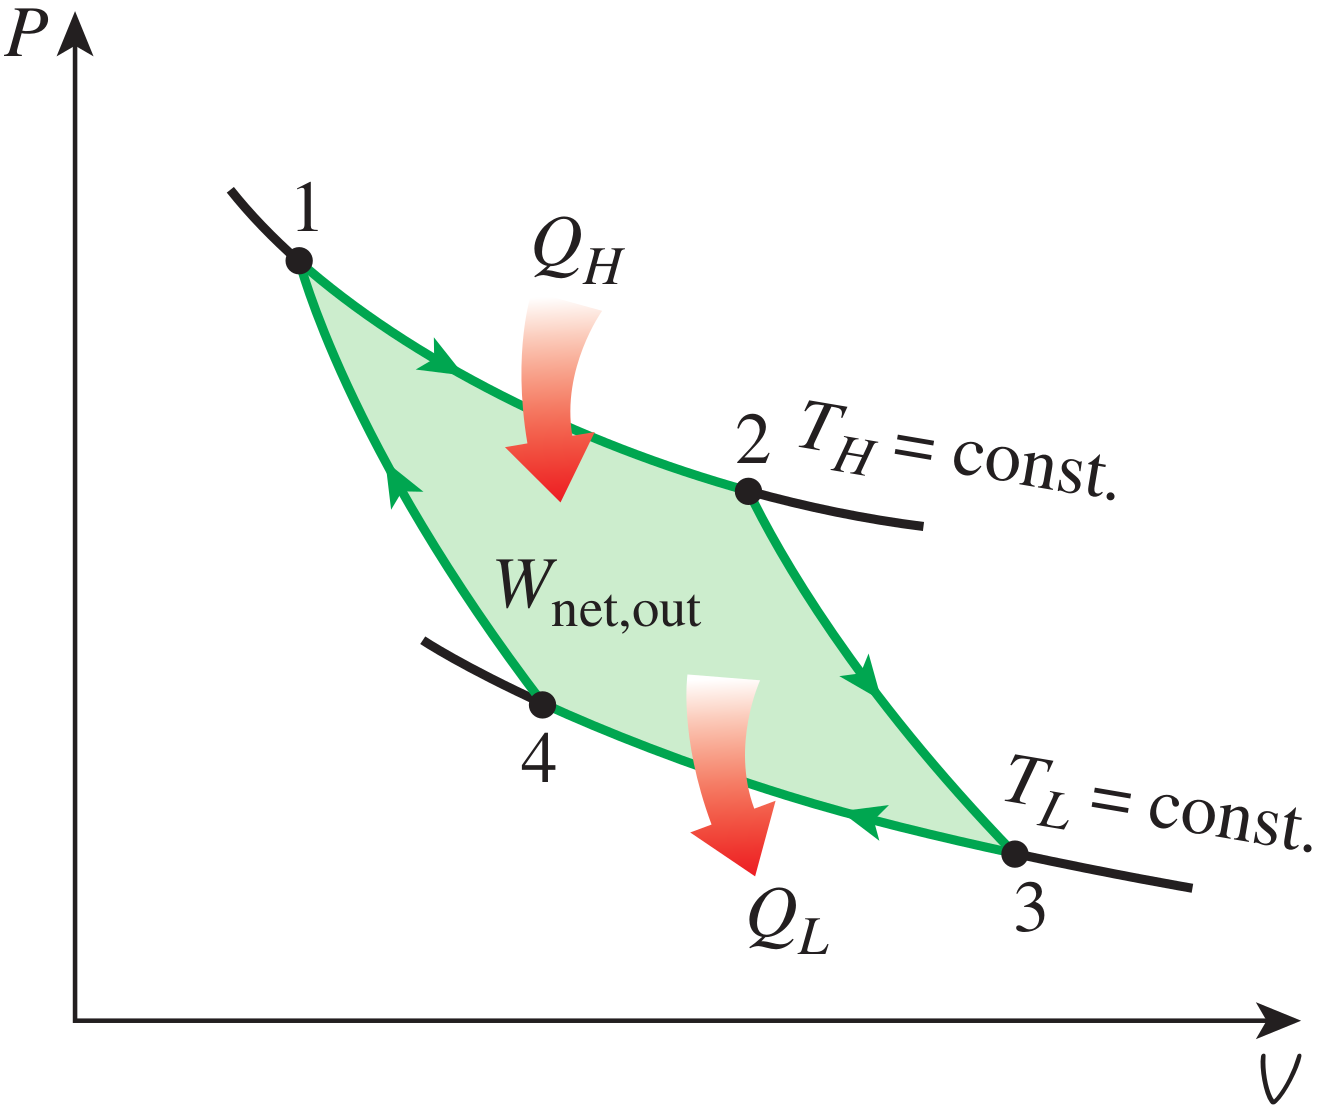
\includegraphics[width=0.5\textwidth]{Carnot_PV.png}
\caption{Carnot cycle - PV diagram \cite{2015}}
\label{fig:C2_CarnotPV}
\end{figure}

Using the first principle, the net work output is equal to $W_{net,out}=Q_H-Q_L$. This means that the efficiency of the cycle is given by
\begin{equation}
\setstretch{1}
\eta_{carnot} = \frac{W_{net,out}}{Q_H} = 1 - \frac{Q_H}{Q_L}
\end{equation} 
Considering that the working fluid is an ideal gas, it can be demonstrated that the heats $Q_H$ and $Q_L$ can be replaced by the corresponding temperature $T_H$ of the hot source and $T_C$ of the cold sink.
\begin{equation}
\setstretch{1}
\eta_{carnot}=1-\frac{T_H}{T_L}\label{eq:C2_eff_carnot}
\end{equation} 
The efficiency of the Carnot cycle is optimal. This implies that for any system playing with a hot source $T_H$ and a cold sink $T_C$, its efficiency cannot be greater than the Carnot efficiency with the \textbf{same} hot source and cold sink temperatures.
\subsection{Entropy}
\quad\, The last lines explained that a system with a hot source $T_H$ and a cold sink $T_C$ will never have a efficiency greater than the Carnot efficiency (for the same source and sink).

For such cycle, it has been demonstrated in 1865 by the German physician R. J. E. Clausius that "the cyclic integral $\oint\frac{\delta Q}{T}$ is always less than or equal to zero"\cite{2015}.
\begin{equation}
\setstretch{1}
\oint\frac{\delta Q}{T} = \frac{Q_H}{T_H} - \frac{Q_L}{T_L}\leq 0\label{eq:C2_cyc}
\end{equation}

For the Carnot cycle, the integral is equal to zeros because the two ratios $\frac{Q_H}{Q_L}$ and $\frac{T_H}{T_L}$ are equal.

From the definition \ref{eq:C2_cyc} can be defined a new state variable named \textbf{entropy}. The entropy S is always measured based on a reference point and, its expression is given in the relation (\ref{eq:C2_S}).
\begin{equation}
\setstretch{1}
dS \triangleq \frac{\delta Q_{rev}}{T}\label{eq:C2_S}
\end{equation}
where $\delta Q_{rev}$ is the "infinitesimal quantity of heat exchanged in a reversible way between the system and the environment at the temperature T"\cite{Dewallef2019}. 

For a reversible adiabatic transformation, the $\delta Q_{rev}=0$. This implies that the entropy remains constant. Such transformations are called \textbf{isentropic} transformation.
\subsection{Second principle definition}
\quad\, Defining the entropy gives a great tool to measure the "quality" of the transformation compared to a similar but reversible transformation.

Based on this definition, one formulation of the second principle of the thermodynamic is that for every transformation, the entropy of the final state of any isolated system is greater or equal to the one of the initial state.

Considering the system defined in the previous lines, it can be said that the increase of entropy $\Delta S_L$ of the cold sink have to be at least greater than the diminution of entropy $\Delta S_H$ of the hot source.

In the case of the Carnot cycle, both variations are equal. This is illustrated on the TS diagram \ref{fig:C2_CarnotTS} where the entropy of state \textbf{1} (resp. state \textbf{2}) is the same as the one of state \textbf{4} (resp. state \textbf{3}).
\begin{figure}[h]
\centering
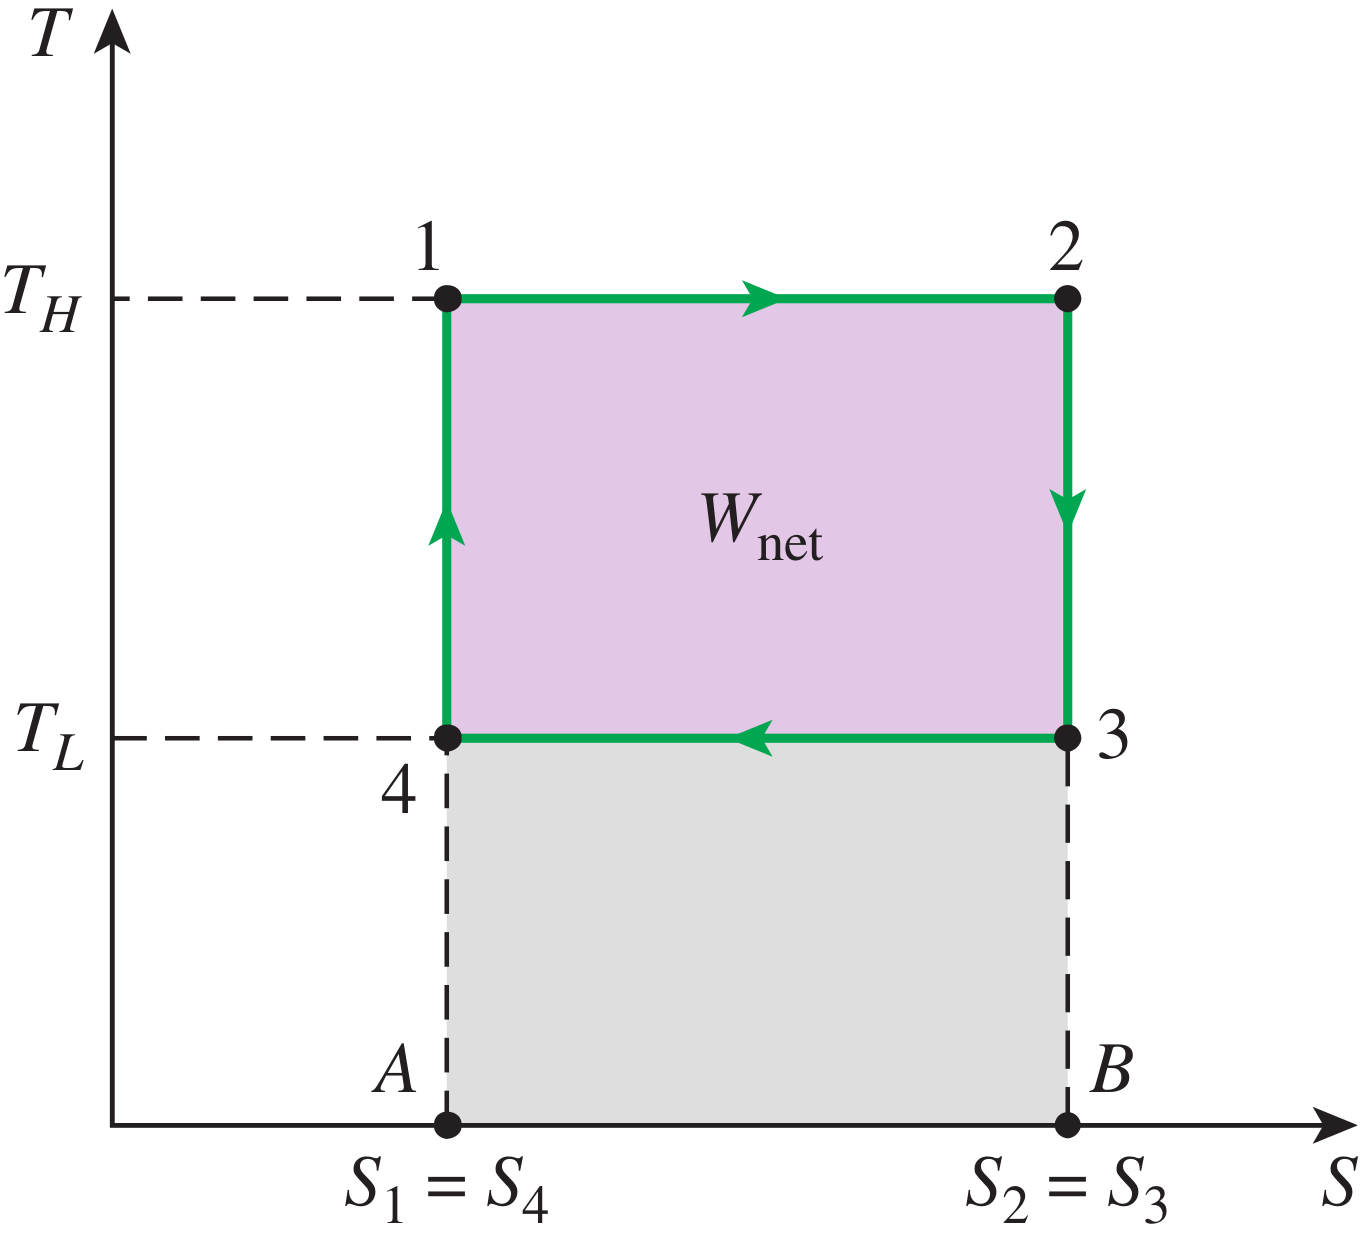
\includegraphics[width=0.5\textwidth]{Carnot_TS.png}
\caption{Carnot cycle - TS diagram \cite{2015}}
\label{fig:C2_CarnotTS}
\end{figure}
\subsection{Computation of the thermodynamic properties}
\quad\, From now, the hypothesis of an ideal gas has been used for the computation of the previously established state variables. However, while this hypothesis remains quite valid when dealing with gas, it cannot be used for a real fluid (e.g. liquid water).

This problem can be solved using the Maxwell relations which provides a linked between the partial derivatives of the state variables $p$, $v$, $T$ and $s$ for a simple compressible system \cite{2015}. 

Those relations can be derived from the four Gibbs relations expressed in (\ref{eq:C2_Gibbs}).

\begin{subequations}
\setstretch{1}
\begin{equation}
  du = Tds - pdv \label{eq:C2_Gibbs1} 
\end{equation}    
\begin{equation}
  dh = Tds + vdp \label{eq:C2_Gibbs2} 
\end{equation}
\begin{equation}
  da = du - Tds - sdT = - pdv - sdT \label{eq:C2_Gibbs3} 
\end{equation}    
\begin{equation}
  dg = dh - Tds - sdT = vdp - sdT \label{eq:C2_Gibbs4}
\end{equation} \label{eq:C2_Gibbs}
\end{subequations}

where the state variables $a$ and $g$ are the Helmholtz and Gibbs function (respectively).

Analyzing the relations allows to notice that each of them are of the form
\begin{align}
\setstretch{1}
dz &= Mdx + Ndy\label{eq:C2_Maxbase}\\
\text{with } \left.\frac{\partial M}{\partial y}\right|_x &= \left.\frac{\partial N}{\partial x}\right|_y\label{eq:C2_partMax}
\end{align}

Using this property, the links between the different state variables are easily obtained by applying the relation (\ref{eq:C2_partMax}) to the equations (\ref{eq:C2_Gibbs1}) to (\ref{eq:C2_Gibbs4}).
\begin{subequations}
\setstretch{1}
\begin{equation}
  \left.\frac{\partial T}{\partial v}\right|_s =  - \left.\frac{\partial p}{\partial s}\right|_v \label{eq:C2_Max1} 
\end{equation}    
\begin{equation}
  \left.\frac{\partial T}{\partial p}\right|_s = \left.\frac{\partial v}{\partial s}\right|_p \label{eq:C2_Max2}  
\end{equation}
\begin{equation}
  \left.\frac{\partial s}{\partial v}\right|_T = \left.\frac{\partial p}{\partial T}\right|_v \label{eq:C2_Max3} 
\end{equation}    
\begin{equation}
  \left.\frac{\partial s}{\partial p}\right|_T =  - \left.\frac{\partial v}{\partial T}\right|_p \label{eq:C2_Max4} 
\end{equation} \label{eq:C2_Max}
\end{subequations}

The relations (\ref{eq:C2_Max}) are called Maxwell equations are helpful in thermodynamics. They provide a method to calculate the variation of the entropy of a system based on the measurement of the variation of the pressure, volume and temperature.

However, this method for calculating the thermodynamic variables is limited to simple compressible system and cannot be used when the system involves "electrical, magnetic, and other effects"\cite{2015}.

These are the relations used when using a digital library for the thermodynamic assessment of the state of a pure fluid with real properties. The open-source library named \textbf{CoolProp}\cite{Bell2014} is one of the best known and. In this work, the library will be called many time when the ideal gas approximation is not relevant.
\subsection{Entropy variation}
\quad\, The previous subsection did introduce the four equations of state (\ref{eq:C2_Gibbs1}) to (\ref{eq:C2_Gibbs4}). Among those, the second equation allows to write the relation (\ref{eq:C2_ds})
\begin{equation}
ds = c_p\frac{dT}{T} - r\frac{dp}{p}\label{eq:C2_ds}
\end{equation}
using the definition (\ref{eq:C2_UP}) of the enthalpy variation and the \textbf{ideal gas equation} (\ref{eq:C2_GP}).

Performing the integration over the path of a transformation going from state \textbf{1} to state \textbf{2}, it can be obtained 
\begin{equation}
s_2 - s_1  = \int_1^2\frac{c_p}{T}dT - r\cdot ln\frac{p_2}{p_1}
\end{equation}
If it is supposed that the variation of the specific heat with respect to temperature are negligible, it can be written
\begin{equation}
s_2 - s_1= r\cdot \left(\frac{k}{k-1}\cdot ln\frac{T_2}{p_1} - ln\frac{p_2}{p_1}\right) = r\cdot ln\left[\frac{p_1}{p_2}\cdot\left(\frac{T_2}{T_1}\right)^\frac{k}{k-1}\right] \label{eq:C2_Deltas}
\end{equation}
where the $c_p=\frac{r\cdot k}{k-1}$ by using the two relations (\ref{eq:C2_r}) and (\ref{eq:C2_k}).

For an isentropic process, the equality $s_2=s_1$ is enforced. Thus, the following relationships can be derived.
\begin{subequations}
\setstretch{1}
\begin{equation}
\frac{p_2}{p_1} = \left(\frac{T_2}{T_1}\right)^\frac{k}{k-1}\label{eq:C2_isrelPT}
\end{equation}
\begin{equation}
\frac{\rho_2}{\rho_1} = \left(\frac{T_2}{T_1}\right)^\frac{1}{k-1}
\label{eq:C2_isrelrhoT}
\end{equation}
\label{eq:C2_isrel}
\end{subequations}
\subsection{Type of transformations}
\quad\, For any transformation from a state \textbf{1} to a state \textbf{2}, it can be defined an efficiency emphasizing how far the transformation is from the ideal transformation. The corresponding ideal transformation will depend on the type of transformation considered.

Mainly, it can be defined 4 ideal transformations.





\subsection{Isentropic efficiency} \label{C2:Isen_eff}
\quad\, For any real transformations, the entropy \textbf{at the end state} is for the major number of cases greater that the one \textbf{at the beginning}. This means that the difference $s_2 - s_1$ is greater than zero.

This can be characterized by defining the isentropic efficiency as being the image of the irreversibilities induced by the transformation. this type of efficiency is very frequently used when studying the compression or the expansion of a fluid.

For a compression or an expansion, the isentropic efficiency is defined by stating that the pressure ratio $\frac{p_1}{p_2}$ is the identical for both the isentropic and non isentropic transformation. Let's substituting this ratio by the constant $\Pi$. 

Considering first the ideal case, the left equality in (\ref{eq:C2_isrel}) gives
\begin{equation}
T_{2,is} = T_1\cdot\Pi^\frac{k-1}{k}
\end{equation}
where the subscript says that the final state is at the same entropy that the starting state.

Then, for the real transformation, the left-hand-side of the relation (\ref{eq:C2_Deltas}) is greater than zero. This implies that
\begin{equation}
T_{2} > T_{2,is} = T_1\cdot\Pi^\frac{k-1}{k}
\end{equation}

As can be noticed, the real transformation leads to a final state temperature bigger than for the isentropic transformation. This difference allows to define the isentropic efficiency $\eta_{is}$. The definition varies based on the desired transformation
\begin{itemize}
\setstretch{1}
\item Compression: $\eta_{is}=\frac{T_{2,is}-T_1}{T_2-T_1}=\frac{h_{2,is}-h_1}{h_2-h_1}$
\item Expansion: $\eta_{is}=\frac{T_1-T_{2}}{T_1-T_{2,is}}=\frac{h_1-h_{2}}{h_1-h_{2,is}}$
\end{itemize}
where the temperature and the enthalpy variation provide the same output result due to the ideal gas hypothesis. For real fluid, the only valid definition of the isentropic efficiency is the one based on the enthalpy variation.

This conclude this second chapter related to the definition of the main thermodynamic notions. While these lines did not cover all the concepts, the minimum have been given to allows the description of the components integrated in the Brayton cycle. 

The next chapter will be devoted to the establishment of these descriptions. For each components, a state of the art and the definitions of the mains concepts will be provided. 

%%%%%%%%%%%%%%%%%%%%%%%%%%%%%%%%%
%% Chapitre 2:                 %%
%% Principles of thermodynamics%%
%%%%%%%%%%%%%%%%%%%%%%%%%%%%%%%%%
\graphicspath{{Chapitre_2_5/Images/}}
\chapter{Principles of thermodynamics}\label{C2_5}
%%%%%%%%%%%%%%%%%%%%%%%%%%%%%%%%%%%
%%%%%                         %%%%%
%%%%%Introduction chapitre 2_5%%%%%
%%%%%                         %%%%%
%%%%%%%%%%%%%%%%%%%%%%%%%%%%%%%%%%%

\quad\ The previous chapter covered many concepts to start analyzing a thermodynamic system submitted to diverse transformations. Among those, the notion of state variables defining the equilibrium state of such system has been defined. 

This chapter will use the first and second principles of the thermodynamic to introduce some state variables that will be used when studying a thermodynamic cycle. Also, a classification of the different transformations will be established.
\section{First principle of thermodynamics}
\quad\ The first principle of thermodynamics state that the energy cannot be created or destroyed, but is rather converted from one form to another.

The chapter \ref{C2} shows that for the general case, the energy balance of a system is given by 

\begin{equation}
  \setstretch{1}
  E_{in} - E_{out} = (Q_{in} - Q_{out}) + (W_{in} - W_{out}) + (E_{mass,in} - E_{mass,out}) = \Delta E_{system} \label{eq:C2_5_EB}
\end{equation}

\subsection{Enthalpy}
\quad\ Considering a closed system, the third term of the energy balance given in the relation(\ref{eq:C2_5_EB}) is nullified. Thus, the variation of the total energy from a state \textbf{1} to a state \textbf{2} is equal to
\begin{equation}
\setstretch{1}
E_{2} - E_{1} = Q_{1-2} - W_{1-2} = m\cdot\left(u_2 - u_1\right) + \frac{1}{2}m\cdot\left(v^2_2 - v^2_1\right) + m\cdot g\cdot\left(z_2 - z1\right)\citep{Dewallef2019} \label{eq:C2_5_EBC}
\end{equation}
Let's note that the terms of kinetic and potential energy are often negligible compared to the internal energy.  

The relation \ref{eq:C2_5_EBC} can be adapted to be applied for the open system by introducing an accumulation term $\Delta E_{cv}$. This correction allows the following reformulation (\ref{eq:C2_5_EBO}) of the energy balance.
\begin{equation}
\setstretch{1}
Q_{1-2} - W_{1-2} - E_{2} - E_{1} = \Delta E_{cv}\label{eq:C2_5_EBO}
\end{equation}

\begin{figure}[h]
\centering
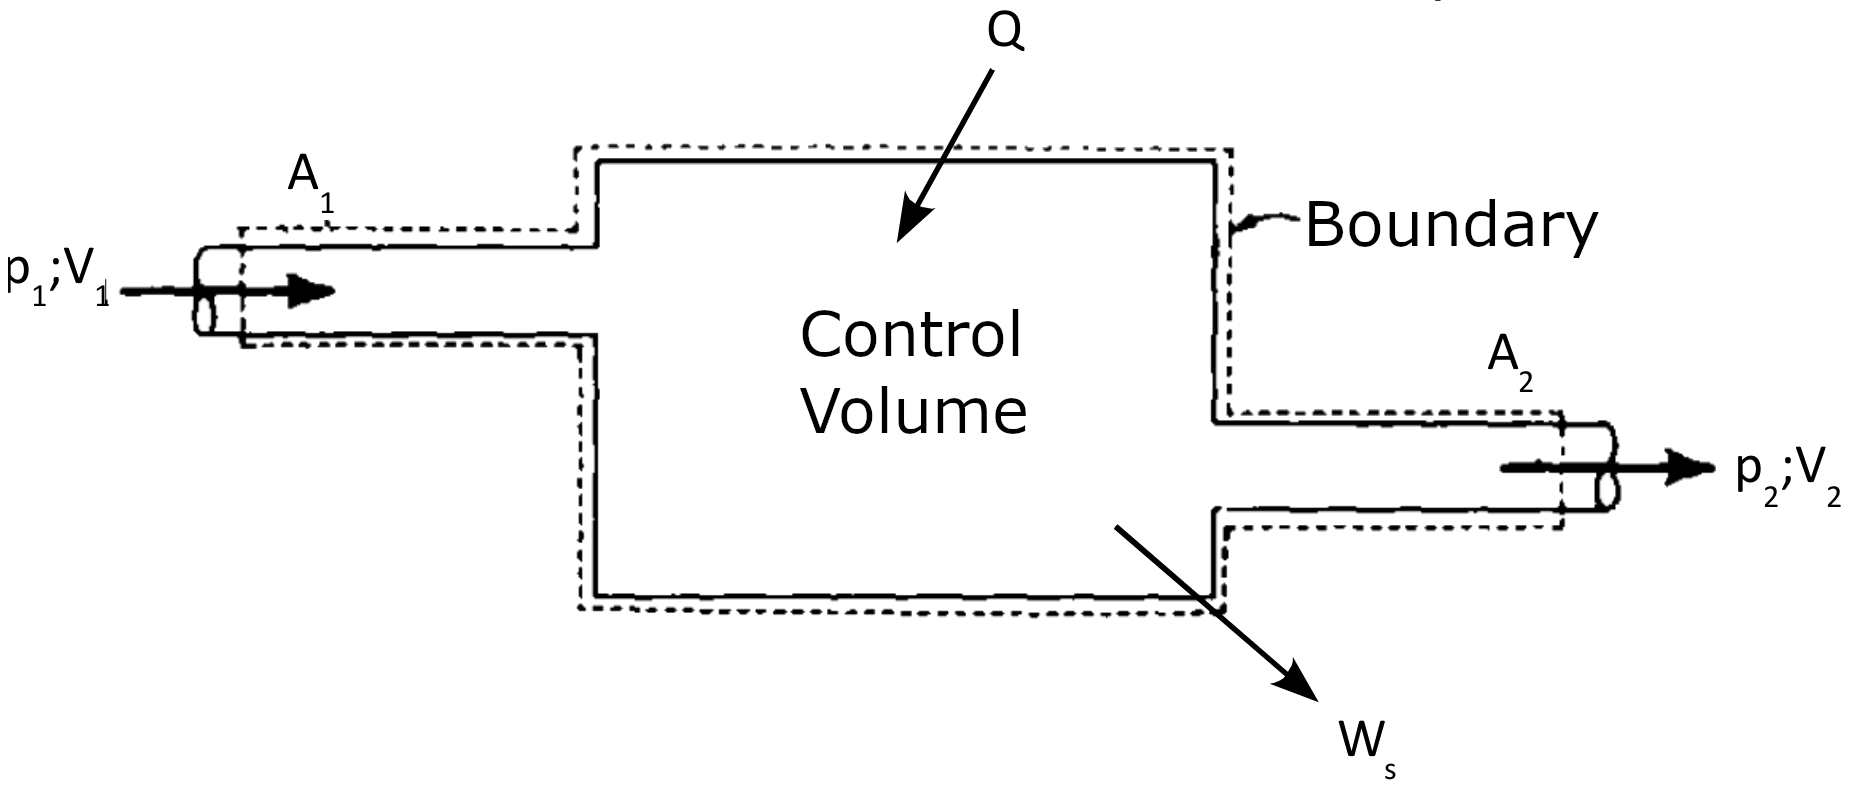
\includegraphics[width=0.7\textwidth]{control_volume.png}
\caption{System control volume \cite{Dewallef2019}.}
\label{fig:C2_5_VC}
\end{figure}

The Figure \ref{fig:C2_5_VC} depicts an open system with an entry and exit area $A_1$ and $A_2$ respectively. Posing that the work $W$ is equal to 
\begin{equation}
\setstretch{1}
W = p_2\cdot A_2\cdot v_2\cdot \Delta t - p_1\cdot A_1\cdot v_1\cdot \Delta t + W_s
\end{equation}      
where $P_1$ (resp. $P_2$) and $v_1$ (resp. $v_2$) are the pressure and the velocity at \textbf{1} (resp. \textbf{2}).

By neglecting the variation of the kinetic and potential energy, the energy balance is after some mathematical operations as given in the relation \ref{eq:C2_5_EBH}
\begin{equation}
\setstretch{1}
q - w_s = u_2 +p_2\cdot \mathrm{v}_2 - u_1 - p_1\cdot \mathrm{v}_1 = h_2 - h_1\label{eq:C2_5_EBH}
\end{equation}
where $q$, $w_s$, and $h$ are respectively the specific work, heat and \textbf{enthalpy} (in J/kg).  

For the case of an ideal gas, the enthalpy and the internal energy only depend on the temperature $T$. Indeed, taking the equation (\ref{eq:C2_5_GP}), the relation (\ref{eq:C2_5_h}) can easily be deduced.
\begin{equation}
\setstretch{1}
h = u(T) + p\cdot \mathrm{v} = u(T) + r\cdot T \label{eq:C2_5_h}
\end{equation}

\subsection{Specific heat}
\quad\ The previous subsection was meant to define the enthalpy. This state variable is used in place of the internal energy when dealing with open system.

An other quantity that is useful for system study is the \textbf{specific heat}. This state variable is defined as the required energy to increase of 1\degree C the temperature of 1kg of a substance. 
 
The required heat to produce this effect depends on the ways the transformation takes place. 
If it is done under constant volume constraint, it is called specific heat at constant volume and denoted $c_v$. 

If the transformation is performed at constant pressure, the symbol associated to the specific heat is $c_p$.
It is worth to note that the specific heat at constant pressure is always higher than the $c_v$. When performing the transformation a constant pressure, the gas expands against the external pressure. This means that the gas does work and, this is the reason behind the greater value of the supplied heat when dealing with a transformation at constant pressure. 

It had been shown that for an ideal gas, the variation of the internal energy can be linked to the specific heat at constant volume as written in the relation (\ref{eq:C2_5_UC}).

\begin{equation}
\setstretch{1}
du = c_vdT \rightarrow u_2 - u_1 = \int_{T_1}^{T_2} c_vdT\label{eq:C2_5_UC}
\end{equation} 

Similarly, the variation of the enthalpy can be expressed using the specific at constant pressure.

\begin{equation}
\setstretch{1}
dh = c_pdT \rightarrow h_2 - h_1 = \int_{T_1}^{T_2} c_pdT\label{eq:C2_5_UP}
\end{equation} 

These two relations, with the equality (\ref{eq:C2_5_h}), provide the required tools to express the gas constant $r$ as a function of the temperature only. 
\begin{equation}
\setstretch{1}
r = c_p - c_v \label{eq:C2_5_r}
\end{equation}

Aside the gas constant, the specific heat ratio $k$ (\ref{eq:C2_5_k}) is also a useful variable to be computed.
\begin{equation}
\setstretch{1}
k = \frac{c_p}{c_v} \label{eq:C2_5_k}
\end{equation}
\subsection{Carnot cycle}
\quad\, The previous subsections used the first principle of the thermodynamic to deduce two useful state variables, namely the enthalpy and the specific heat.

Now, let's move aside those notions and let consider the case where the transformation applied to a system is reversible. A necessary condition for the reversibility is that the transformation has to be done in quasi-equilibrium. This implies that if the transformation is reversed, the system goes back to its initial state.


\begin{figure}[h]
\centering
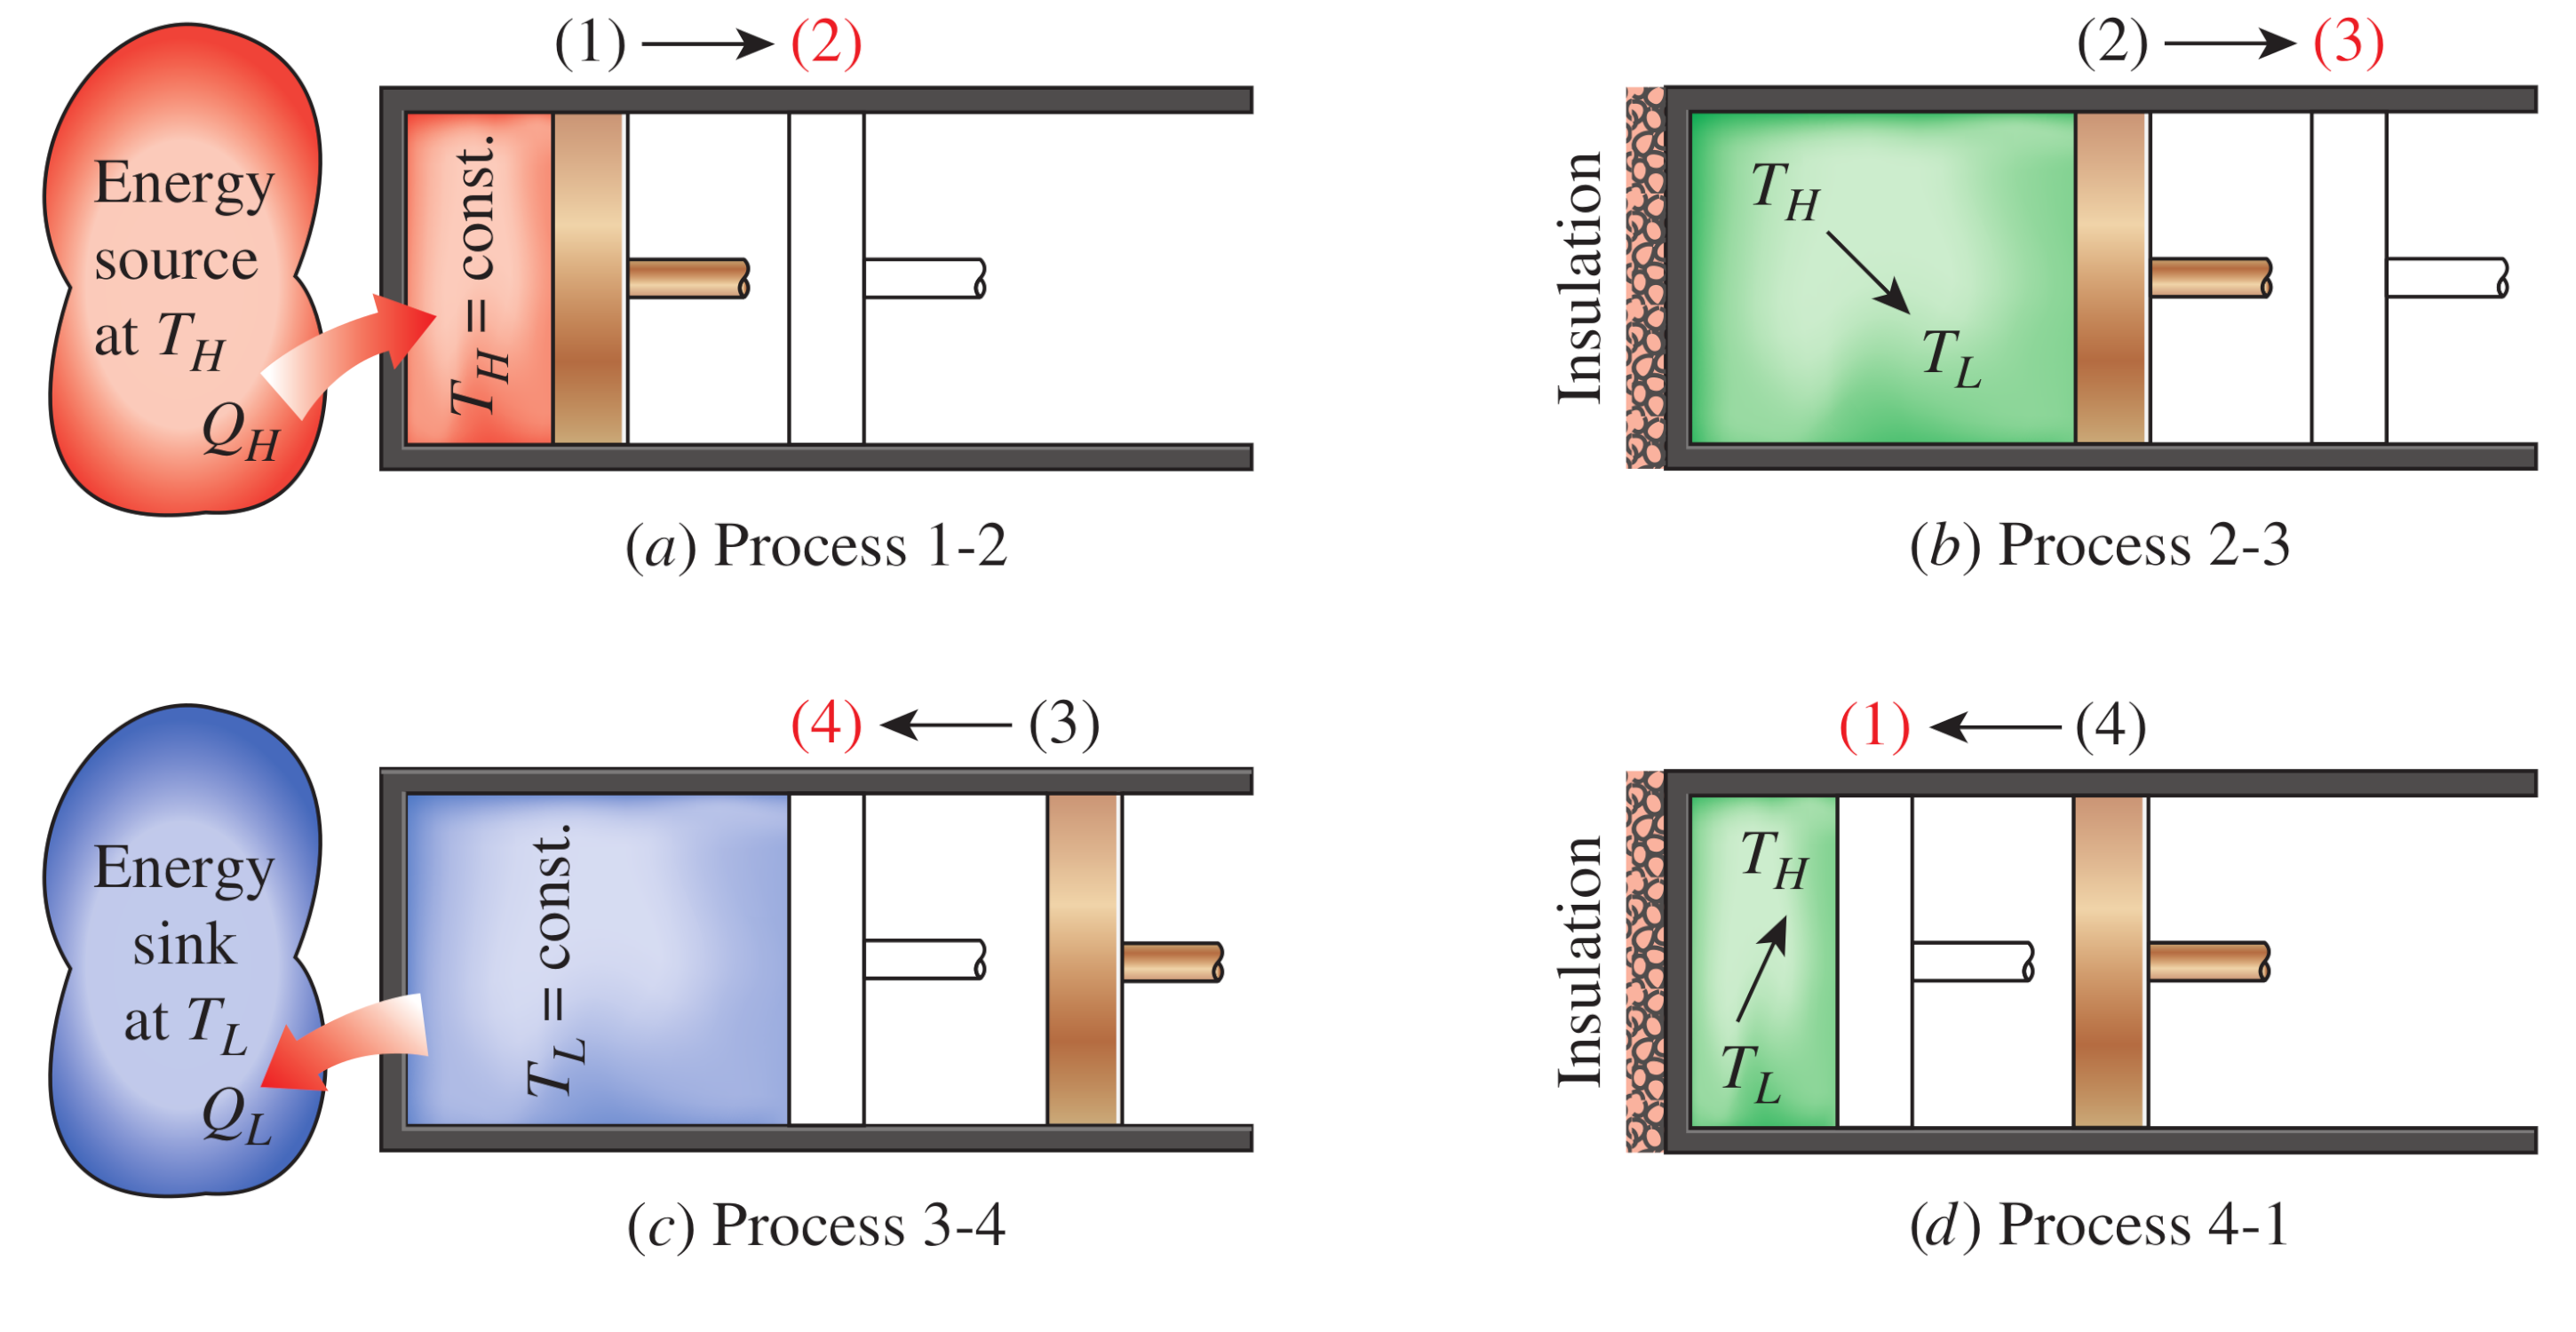
\includegraphics[width=0.7\textwidth]{Carnot_schema.png}
\caption{Carnot cycle - Schematic \cite{2015}.}
\label{fig:C2_5_Carnot}
\end{figure}
The Carnot cycle is a thermodynamic cycle composed of 4 reversible transformations illustrated on Figure \ref{fig:C2_5_Carnot}. The transformations are defined as follows.

\begin{itemize}
\setstretch{1}
\item \textbf{1} to \textbf{2} (Figure \ref{fig:C2_5_Carnot}a): Reversible isothermal expansion with a heat transfer $Q_H$ from the environment to the system
\item \textbf{2} to \textbf{3} (Figure \ref{fig:C2_5_Carnot}b): Reversible  adiabatic expansion
\item \textbf{3} to \textbf{4} (Figure \ref{fig:C2_5_Carnot}c): Reversible isothermal compression with a heat transfer $Q_L$ from the system to the environment
\item \textbf{4} to \textbf{1} (Figure \ref{fig:C2_5_Carnot}d): Reversible adiabatic compression
\end{itemize}

For visual representation, this cycle has been represented in the PV diagram \ref{fig:C2_5_CarnotPV} where the different transformations are well exposed.
\begin{figure}[h]
\centering
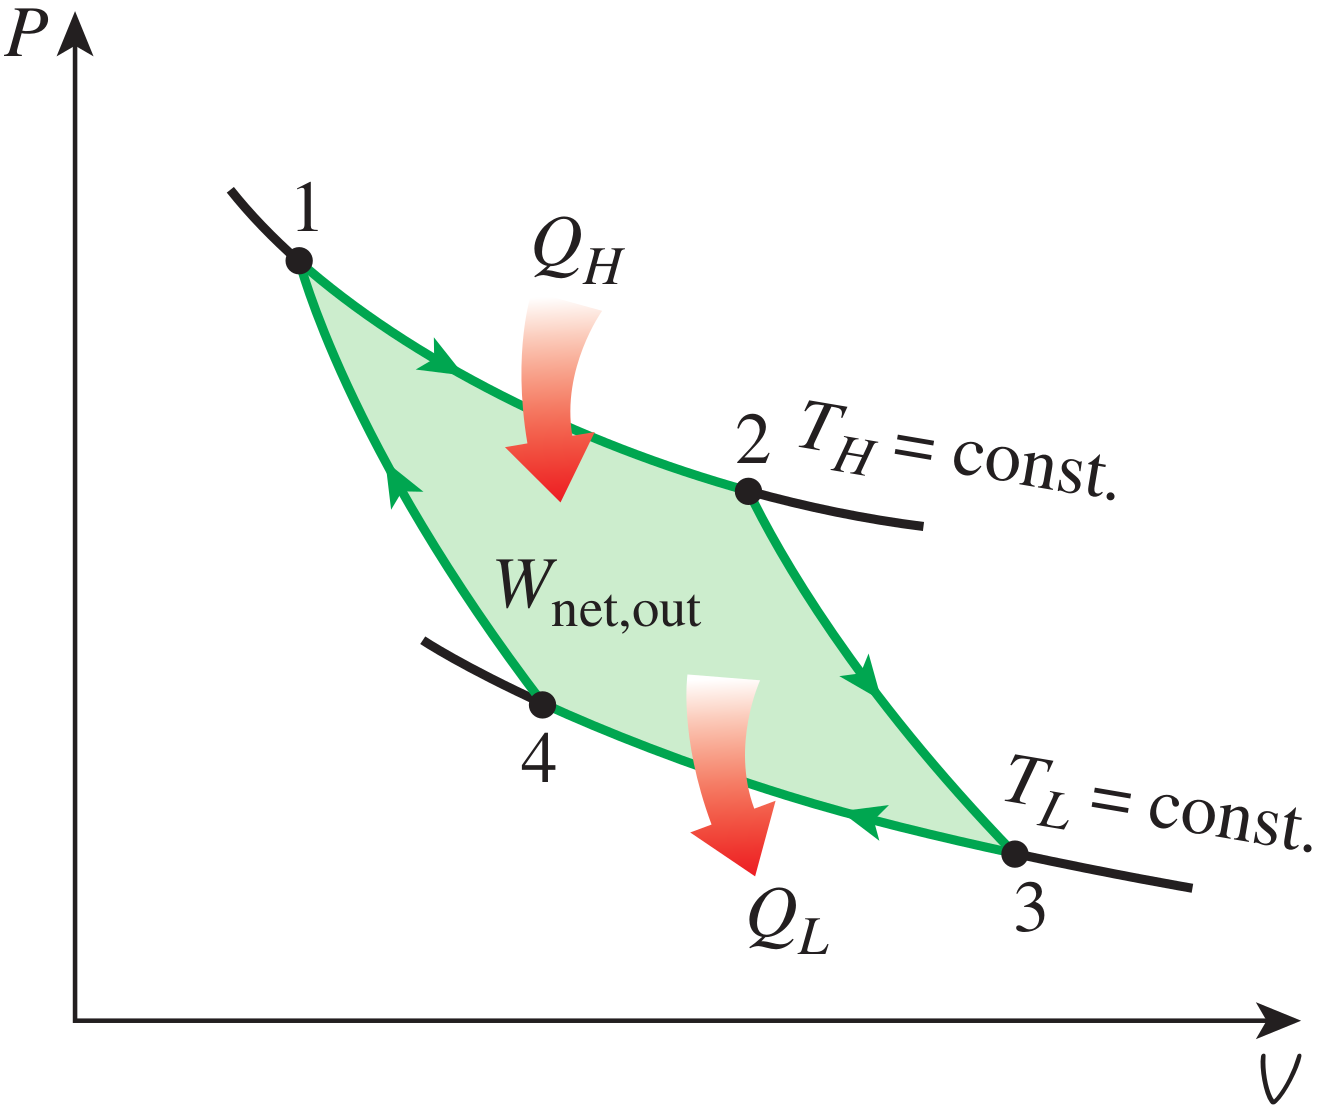
\includegraphics[width=0.5\textwidth]{Carnot_PV.png}
\caption{Carnot cycle - PV diagram \cite{2015}.}
\label{fig:C2_5_CarnotPV}
\end{figure}

Using the first principle, the net work output is equal to $W_{net,out}=Q_H-Q_L$. This means that the efficiency of the cycle is given by

\begin{equation}
\setstretch{1}
\eta_{carnot} = \frac{W_{net,out}}{Q_H} = 1 - \frac{Q_H}{Q_L}
\end{equation} 

Considering that the working fluid is an ideal gas, it can be demonstrated that the heats $Q_H$ and $Q_L$ can be replaced by the corresponding temperature $T_H$ of the hot source and $T_C$ of the cold sink.

\begin{equation}
\setstretch{1}
\eta_{carnot}=1-\frac{T_H}{T_L}\label{eq:C2_5_eff_carnot}
\end{equation} 
The efficiency of the Carnot cycle is optimal. This implies that for any system playing with a hot source $T_H$ and a cold sink $T_C$, its efficiency cannot be greater than the Carnot efficiency with the \textbf{same} hot source and cold sink temperatures.

\subsection{Entropy}
\quad\ The last lines explained that a system with a hot source $T_H$ and a cold sink $T_C$ will never have a efficiency greater than the Carnot efficiency (for the same source and sink).

For such cycle, it has been demonstrated in 1865 by the German physician R. J. E. Clausius that "the cyclic integral $\oint\frac{\delta Q}{T}$ is always less than or equal to zero"\cite{2015}.
\begin{equation}
\setstretch{1}
\oint\frac{\delta Q}{T} = \frac{Q_H}{T_H} - \frac{Q_L}{T_L}\leq 0\label{eq:C2_5_cyc}
\end{equation}

For the Carnot cycle, the integral is equal to zeros because the two ratios $\frac{Q_H}{Q_L}$ and $\frac{T_H}{T_L}$ are equal.

From the definition \ref{eq:C2_5_cyc} can be defined a new state variable named \textbf{entropy}. The entropy S is always measured based on a reference point and, its expression is given in the relation (\ref{eq:C2_5_S}).
\begin{equation}
\setstretch{1}
dS \triangleq \frac{\delta Q_{rev}}{T}\label{eq:C2_5_S}
\end{equation}
where $\delta Q_{rev}$ is the "infinitesimal quantity of heat exchanged in a reversible way between the system and the environment at the temperature T"\cite{Dewallef2019}. 

For a reversible adiabatic transformation, the $\delta Q_{rev}=0$. This implies that the entropy remains constant. Such transformations are called \textbf{isentropic} transformation.
\begin{figure}[h]
\centering
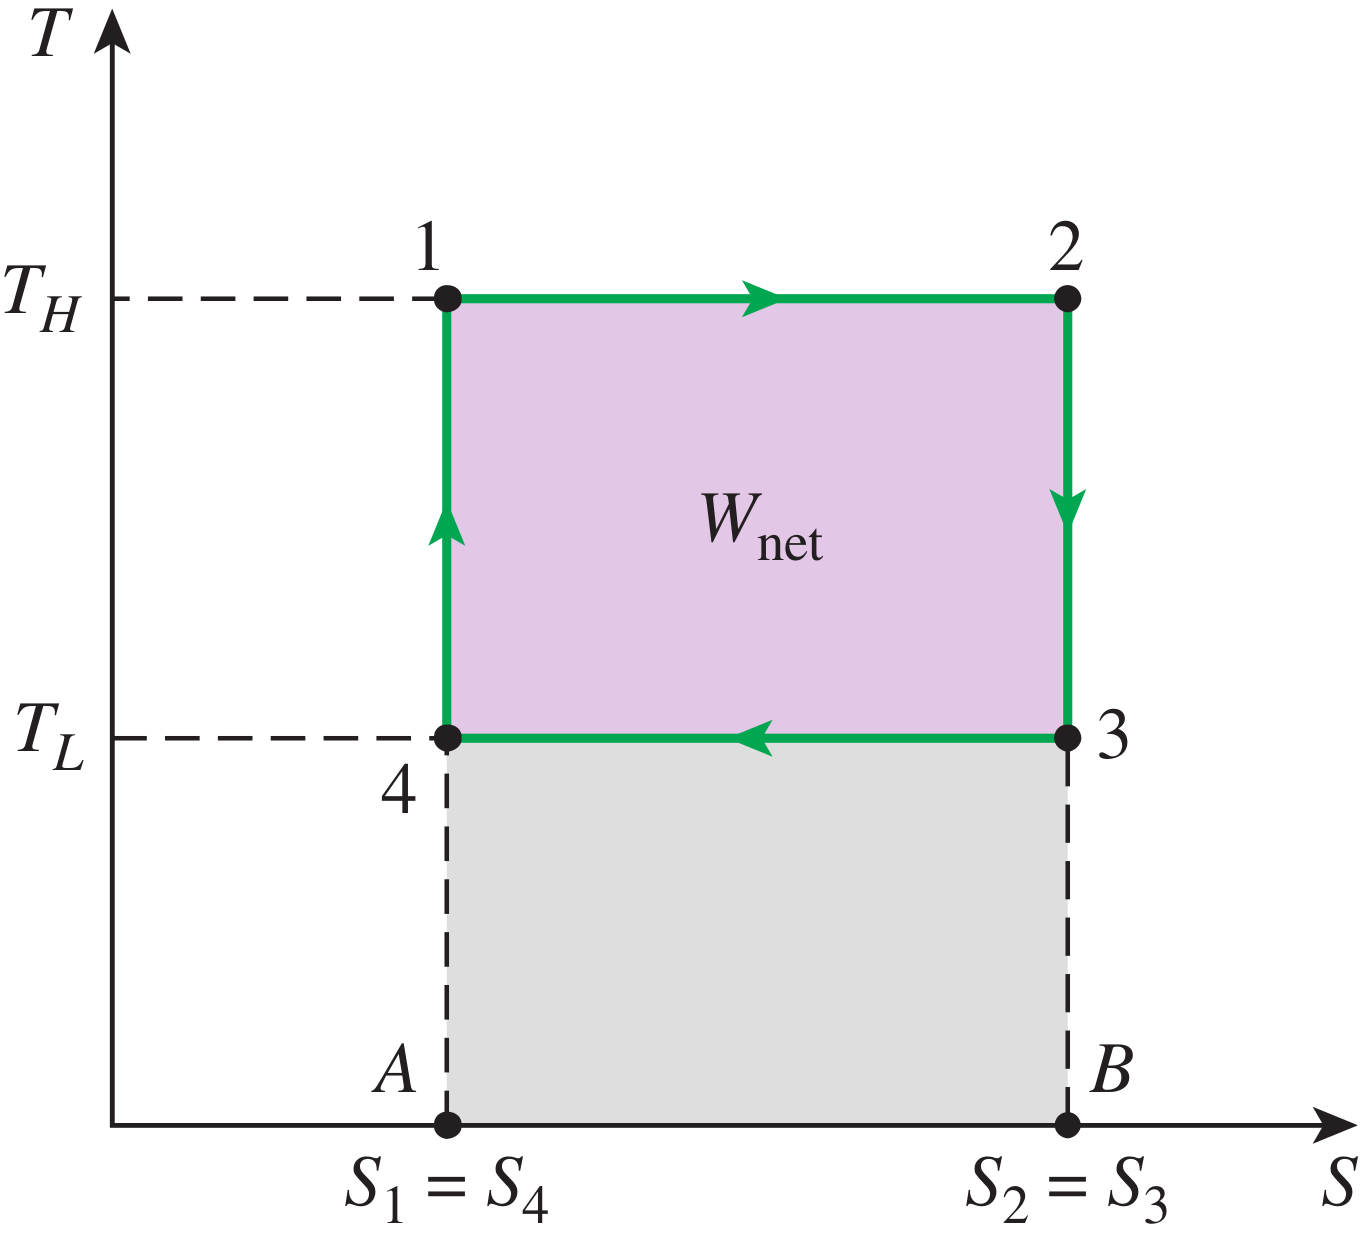
\includegraphics[width=0.5\textwidth]{Carnot_TS.png}
\caption{Carnot cycle - TS diagram \cite{2015}.}
\label{fig:C2_5_CarnotTS}
\end{figure}
\section{Second principle definition}
\quad\, Defining the entropy gives a great tool to measure the "quality" of the transformation compared to a similar but reversible transformation.

Based on this definition, one formulation of the second principle of the thermodynamic is that for every transformation, the entropy of the final state of any isolated system is greater or equal to the one of the initial state.

Considering the system defined in the previous lines, it can be said that the increase of entropy $\Delta S_L$ of the cold sink have to be at least greater than the diminution of entropy $\Delta S_H$ of the hot source.

In the case of the Carnot cycle, both variations are equal. This is illustrated on the TS diagram \ref{fig:C2_5_CarnotTS} where the entropy of state \textbf{1} (resp. state \textbf{2}) is the same as the one of state \textbf{4} (resp. state \textbf{3}).

\section{Type of reversible transformations}
\quad\ During this chapter, it has been mentioned several time the notions of reversible processes. 

As it has been explained, a transformation is said reversible if it takes an infinite amount of time to bring the system from its initial state \textbf{1} to its final state \textbf{2}. The different type of transformation are going to be described in the section.

\subsection{Isothermal transformation}
\begin{wrapfigure}{l}{0.45\linewidth}
  \centering
  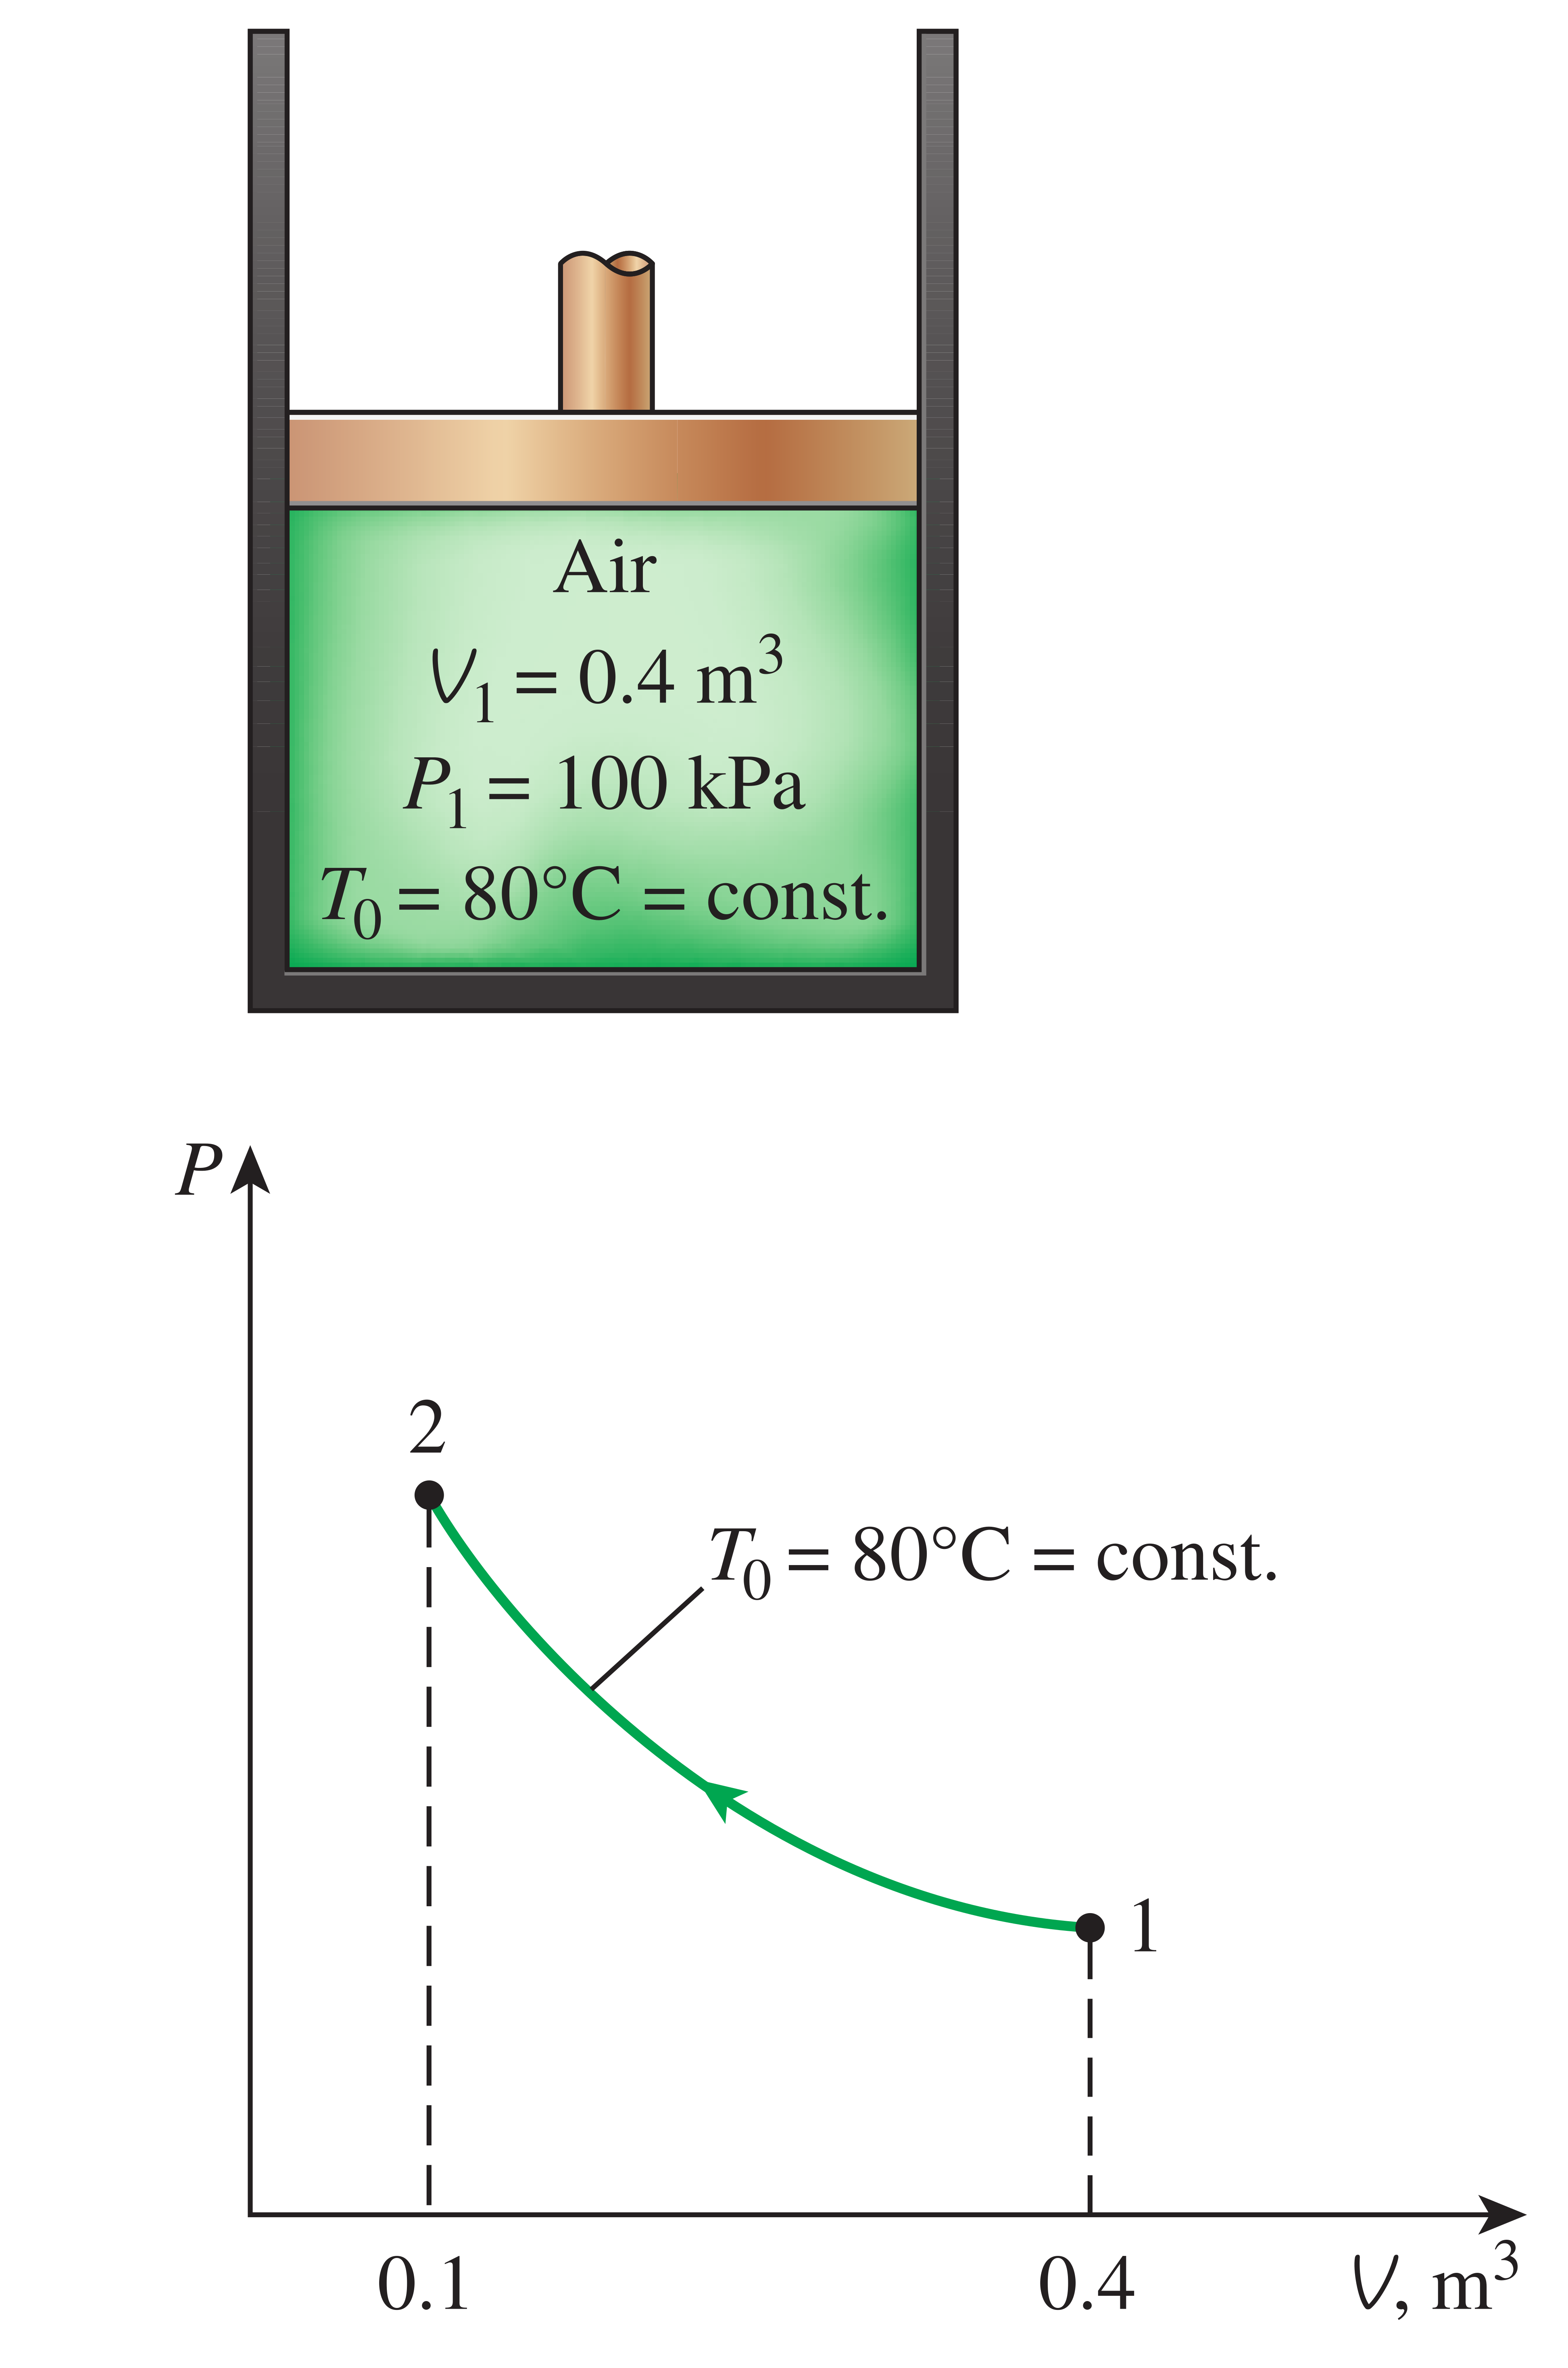
\includegraphics{isoT.png}
  \caption{Isothermal transformation \cite{2015}.}
  \label{fig:C2_5_isoT}
  \end{wrapfigure}
\quad\ The first type of transformations to be considered are the isothermal processes. Here, considering that the transformation bring the system from state \textbf{1} to \textbf{2}, the equality \(T_2 = T_1\)  is enforced. 

The transformation is said reversible isothermal if during all the process the temperature remains constant. Such transformation is depicted on Figure \ref{fig:C2_5_isoT}. The ideal gas equation (\ref{eq:C2_GP}) allows to derive the relation (\ref{eq:C2_5_isoT}) if the mass within the system does not vary.

\setstretch{1}
  \begin{align}
    p_1\cdot \mathrm{V}_1 &= p_2\cdot \mathrm{V}_2\nonumber\\
    \rightarrow p\cdot \mathrm{V} &= C \label{eq:C2_5_isoT}  
  \end{align}
\setstretch{1.5}


 For a compression (resp. an expansion), the process is said isothermal if the system is cooled (resp. heat up) to bring the final state temperature to its initial value.

Considering an isothermal compression, the boundary work $W_b$, corresponding to the area below the curve, is given in the development (\ref{eq:C2_5_WbisoT})
\begin{align}
  \setstretch{1}
  W_b &= \int_1^2 pd\mathrm{V} = C\cdot\int_1^2d\mathrm{V}\nonumber\\
  &= C\cdot \ln \frac{V_2}{V_1} = p_1\cdot V_1\cdot \ln \frac{V_2}{V_1} \label{eq:C2_5_WbisoT}
\end{align} 
\subsection{Isobaric transformation}
\begin{wrapfigure}{r}{0.45\linewidth}
  \centering
  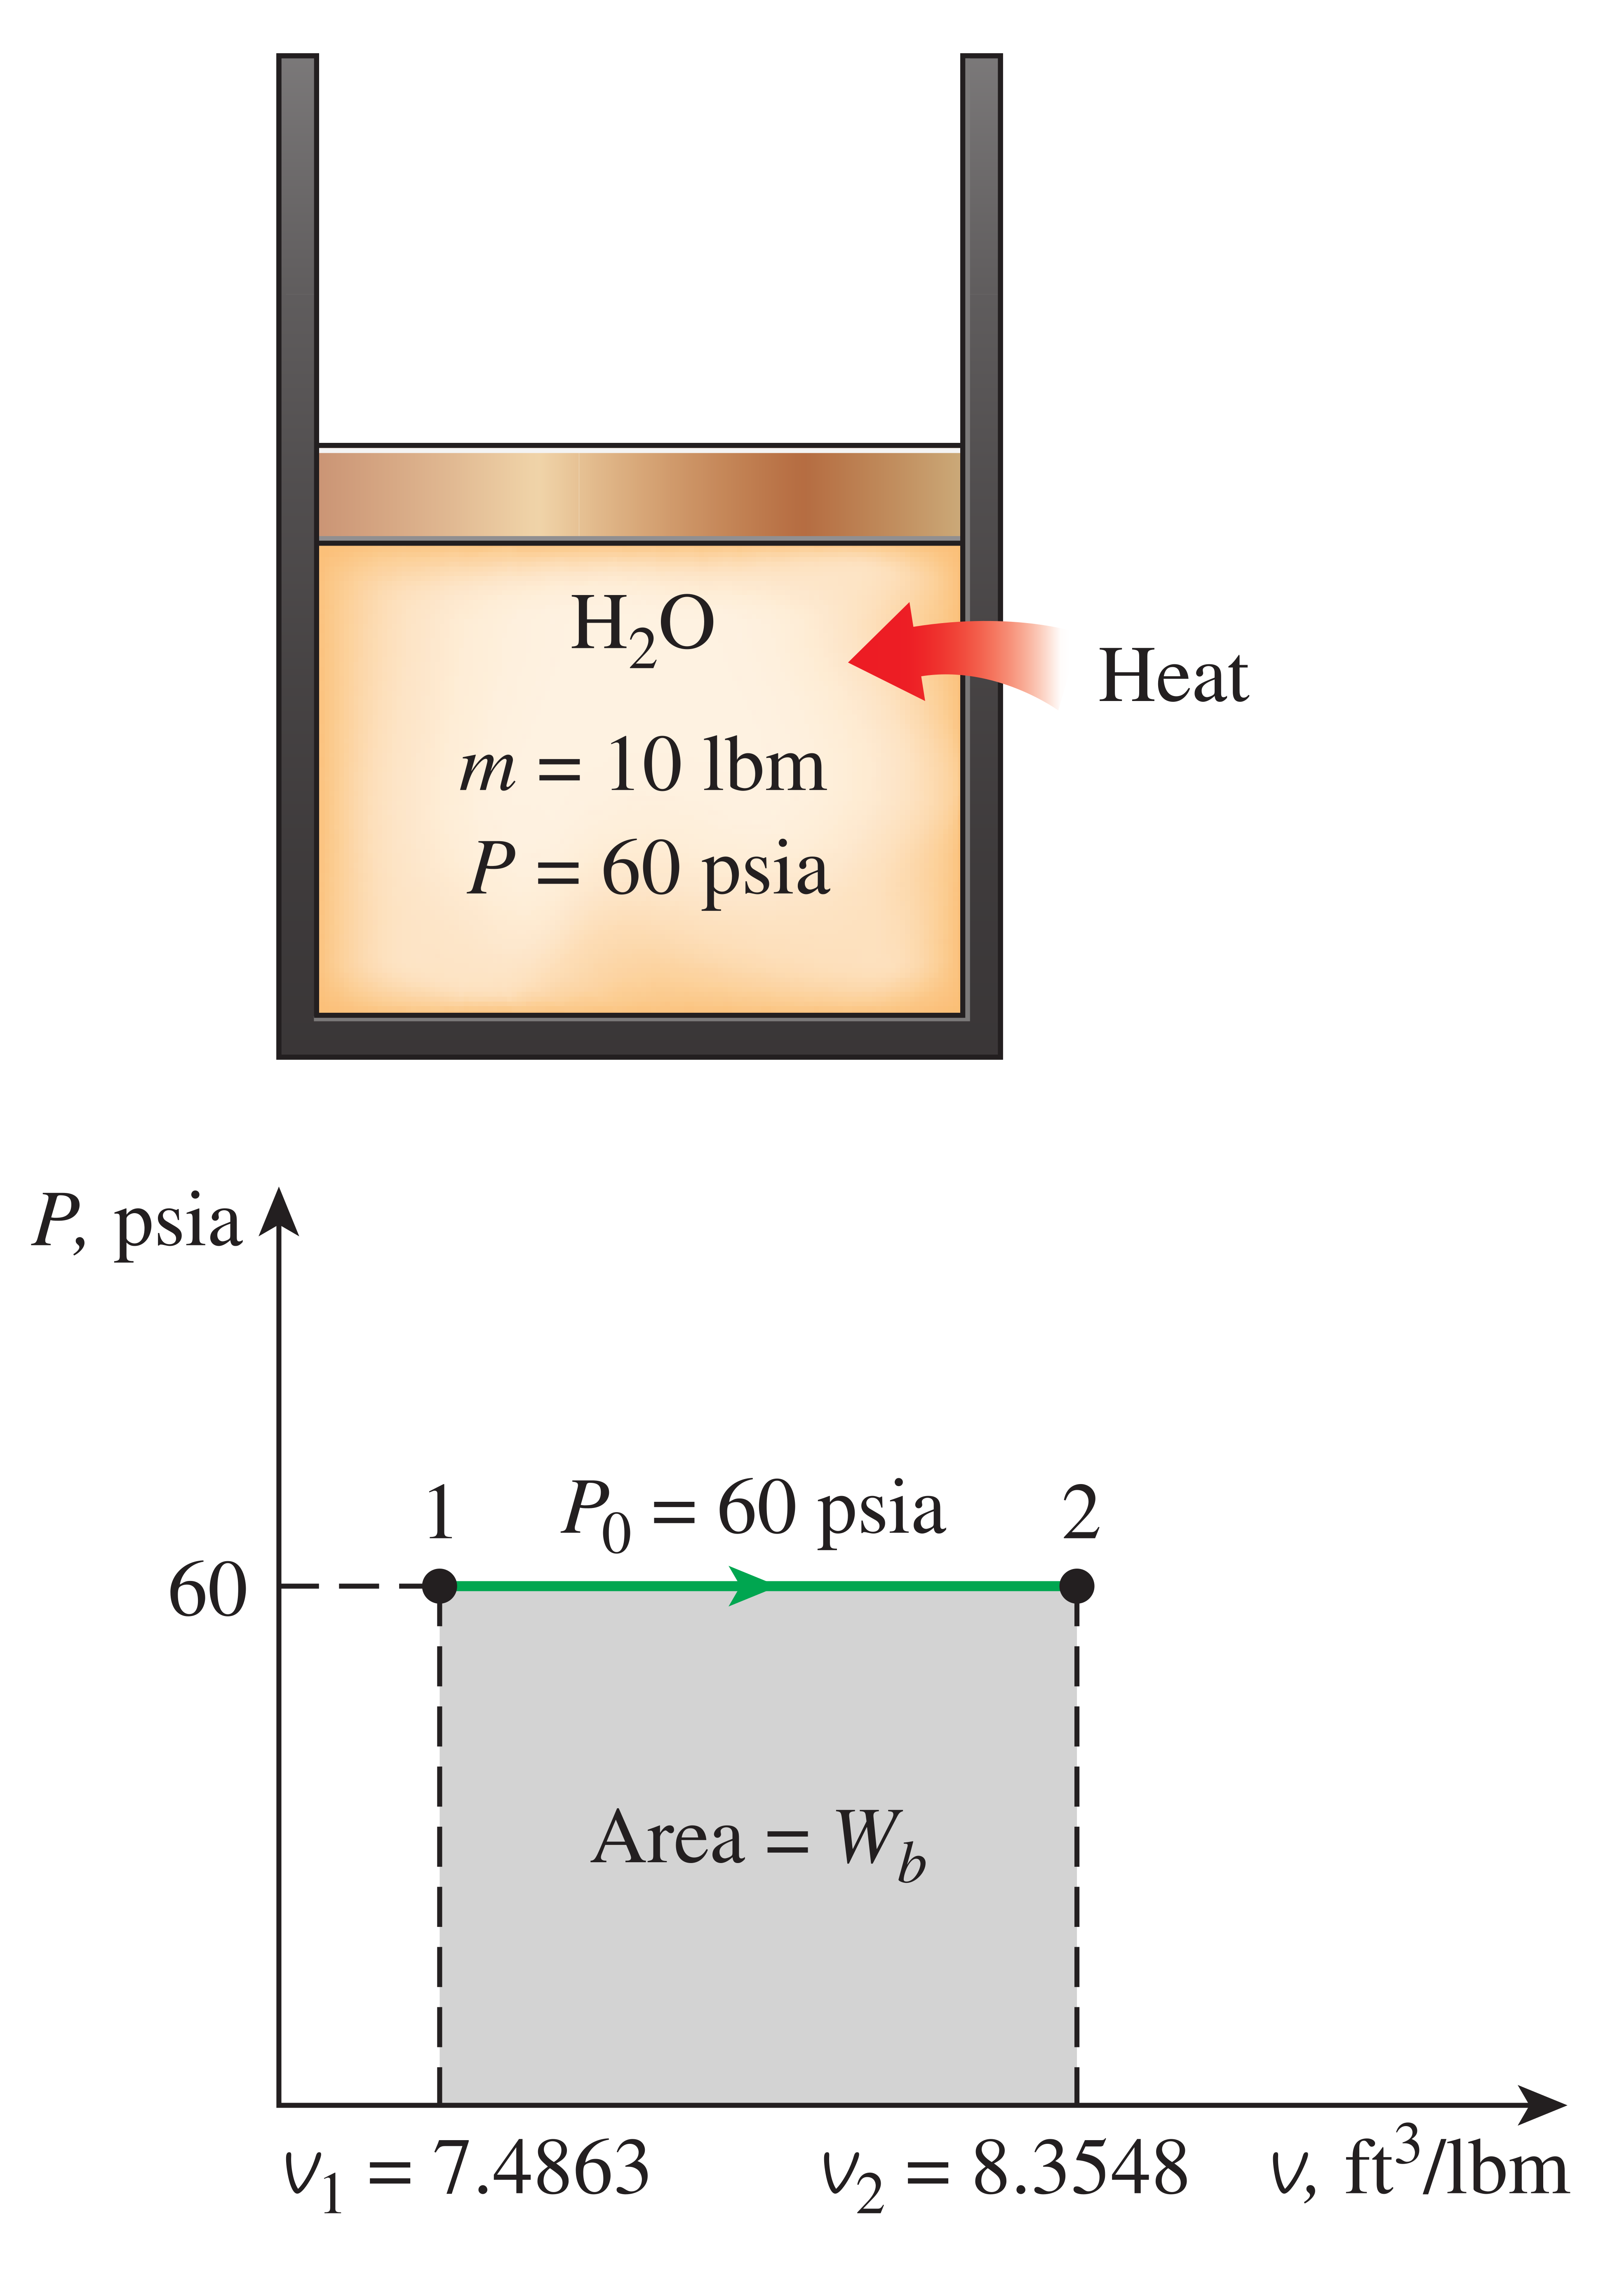
\includegraphics{isoP.png}
  \caption{Isobaric transformation \cite{2015}.}
  \label{fig:C2_5_isoB}
\end{wrapfigure}
\quad\ The isobaric transformation are one for which the initial and final state are both characterized by the same pressure. Thus, the equality \(p_2 = p_1 = p_0\). Figure \ref{fig:C2_5_isoB} illustrates such transformation.

Typically, the transformation within the combustion chamber, heat exchanger or piping aim to be as closed as this transformation. Diverging from this ideal transformation implies that the component induces some pressure losses.

As for the isothermal transformation, the boundary work for an isobaric transformation is equal to the area below the curve. Here, the expression is

\setstretch{1}
\begin{align}
  W_b &= p_0\cdot \int_1^2d\mathrm{V}\nonumber\\
   &= p_0\cdot (\mathrm{V_2} - \mathrm{V_1}) = m\cdot p_0\cdot (\mathrm{v_2} - \mathrm{v_1})
\end{align}
\setstretch{1.5}
\newpage

\subsection{Polytropic transformation}
\begin{wrapfigure}{l}{0.45\linewidth}
  \centering
  \includegraphics{poly.png}
  \caption{Polytropic transformation \cite{2015}.}
  \label{fig:C2_5_poly}
\end{wrapfigure}
\quad\ The polytropic transformation, depicted on Figure \ref{fig:C2_5_poly}, is  generalization of the isothermal transformation. For an ideal gas, the polytropic transformation is characterized by the relation (\ref{eq:C2_5_poly}).

\begin{equation}
  p\cdot \mathrm{V}^n = C \label{eq:C2_5_poly}
\end{equation}

where $n$ is a constant. For $n=1$, the transformation simply correspond to the isothermal transformation.

\subsection{Isentropic transformation}
\quad\ The last transformation to be considered is the isentropic transformation. This transformation corresponds to a reversible adiabatic transformation. 

Typically, when considering the expansion or the compression of a fluid, the manufacturers aim to build a machine which tends to minimize as much as possible the irreversibilities. 

On Figures \ref{fig:C2_5_isen} and \ref{fig:C2_5_isreal} are respectively depicted an isentropic and a real expansion. As it can be   
\section{Isentropic efficiency} \label{C2_5:Isen_eff}
\quad\, For any real transformations, the entropy \textbf{at the end state} is for the major number of cases greater that the one \textbf{at the beginning}. This means that the difference $s_2 - s_1$ is greater than zero.

This can be characterized by defining the isentropic efficiency as being the image of the irreversibilities induced by the transformation. this type of efficiency is very frequently used when studying the compression or the expansion of a fluid.

For a compression or an expansion, the isentropic efficiency is defined by stating that the pressure ratio $\frac{p_1}{p_2}$ is the identical for both the isentropic and non isentropic transformation. Let's substituting this ratio by the constant $\Pi$. 

Considering first the ideal case, the left equality in (\ref{eq:C2_5_isrel}) gives
\begin{equation}
T_{2,is} = T_1\cdot\Pi^\frac{k-1}{k}
\end{equation}
where the subscript says that the final state is at the same entropy that the starting state.

Then, for the real transformation, the left-hand-side of the relation (\ref{eq:C2_5_Deltas}) is greater than zero. This implies that
\begin{equation}
T_{2} > T_{2,is} = T_1\cdot\Pi^\frac{k-1}{k}
\end{equation}

As can be noticed, the real transformation leads to a final state temperature bigger than for the isentropic transformation. This difference allows to define the isentropic efficiency $\eta_{is}$. The definition varies based on the desired transformation
\begin{itemize}
\setstretch{1}
\item Compression: $\eta_{is}=\frac{T_{2,is}-T_1}{T_2-T_1}=\frac{h_{2,is}-h_1}{h_2-h_1}$
\item Expansion: $\eta_{is}=\frac{T_1-T_{2}}{T_1-T_{2,is}}=\frac{h_1-h_{2}}{h_1-h_{2,is}}$
\end{itemize}
where the temperature and the enthalpy variation provide the same output result due to the ideal gas hypothesis. For real fluid, the only valid definition of the isentropic efficiency is the one based on the enthalpy variation.






\section{Computation of the thermodynamic properties}
\quad\, From now, the hypothesis of an ideal gas has been used for the computation of the previously established state variables. However, while this hypothesis remains quite valid when dealing with gas, it cannot be used for a real fluid (e.g. liquid water).

This problem can be solved using the Maxwell relations which provides a linked between the partial derivatives of the state variables $p$, $v$, $T$ and $s$ for a simple compressible system \cite{2015}. 

Those relations can be derived from the four Gibbs relations expressed in (\ref{eq:C2_5_Gibbs}).

\begin{subequations}
\setstretch{1}
\begin{equation}
  du = Tds - pdv \label{eq:C2_5_Gibbs1} 
\end{equation}    
\begin{equation}
  dh = Tds + vdp \label{eq:C2_5_Gibbs2} 
\end{equation}
\begin{equation}
  da = du - Tds - sdT = - pdv - sdT \label{eq:C2_5_Gibbs3} 
\end{equation}    
\begin{equation}
  dg = dh - Tds - sdT = vdp - sdT \label{eq:C2_5_Gibbs4}
\end{equation} \label{eq:C2_5_Gibbs}
\end{subequations}

where the state variables $a$ and $g$ are the Helmholtz and Gibbs function (respectively).

Analyzing the relations allows to notice that each of them are of the form
\begin{align}
\setstretch{1}
dz &= Mdx + Ndy\label{eq:C2_5_Maxbase}\\
\text{with } \left.\frac{\partial M}{\partial y}\right|_x &= \left.\frac{\partial N}{\partial x}\right|_y\label{eq:C2_5_partMax}
\end{align}

Using this property, the links between the different state variables are easily obtained by applying the relation (\ref{eq:C2_5_partMax}) to the equations (\ref{eq:C2_5_Gibbs1}) to (\ref{eq:C2_5_Gibbs4}).
\begin{subequations}
\setstretch{1}
\begin{equation}
  \left.\frac{\partial T}{\partial v}\right|_s =  - \left.\frac{\partial p}{\partial s}\right|_v \label{eq:C2_5_Max1} 
\end{equation}    
\begin{equation}
  \left.\frac{\partial T}{\partial p}\right|_s = \left.\frac{\partial v}{\partial s}\right|_p \label{eq:C2_5_Max2}  
\end{equation}
\begin{equation}
  \left.\frac{\partial s}{\partial v}\right|_T = \left.\frac{\partial p}{\partial T}\right|_v \label{eq:C2_5_Max3} 
\end{equation}    
\begin{equation}
  \left.\frac{\partial s}{\partial p}\right|_T =  - \left.\frac{\partial v}{\partial T}\right|_p \label{eq:C2_5_Max4} 
\end{equation} \label{eq:C2_5_Max}
\end{subequations}

The relations (\ref{eq:C2_5_Max}) are called Maxwell equations are helpful in thermodynamics. They provide a method to calculate the variation of the entropy of a system based on the measurement of the variation of the pressure, volume and temperature.

However, this method for calculating the thermodynamic variables is limited to simple compressible system and cannot be used when the system involves "electrical, magnetic, and other effects"\cite{2015}.

These are the relations used when using a digital library for the thermodynamic assessment of the state of a pure fluid with real properties. The open-source library named \textbf{CoolProp}\cite{Bell2014} is one of the best known and. In this work, the library will be called many time when the ideal gas approximation is not relevant.
\section{Entropy variation}
\quad\, The previous subsection did introduce the four equations of state (\ref{eq:C2_5_Gibbs1}) to (\ref{eq:C2_5_Gibbs4}). Among those, the second equation allows to write the relation (\ref{eq:C2_5_ds})
\begin{equation}
ds = c_p\frac{dT}{T} - r\frac{dp}{p}\label{eq:C2_5_ds}
\end{equation}
using the definition (\ref{eq:C2_5_UP}) of the enthalpy variation and the \textbf{ideal gas equation} (\ref{eq:C2_5_GP}).

Performing the integration over the path of a transformation going from state \textbf{1} to state \textbf{2}, it can be obtained 
\begin{equation}
s_2 - s_1  = \int_1^2\frac{c_p}{T}dT - r\cdot ln\frac{p_2}{p_1}
\end{equation}
If it is supposed that the variation of the specific heat with respect to temperature are negligible, it can be written
\begin{equation}
s_2 - s_1= r\cdot \left(\frac{k}{k-1}\cdot ln\frac{T_2}{p_1} - ln\frac{p_2}{p_1}\right) = r\cdot ln\left[\frac{p_1}{p_2}\cdot\left(\frac{T_2}{T_1}\right)^\frac{k}{k-1}\right] \label{eq:C2_5_Deltas}
\end{equation}
where the $c_p=\frac{r\cdot k}{k-1}$ by using the two relations (\ref{eq:C2_5_r}) and (\ref{eq:C2_5_k}).

For an isentropic process, the equality $s_2=s_1$ is enforced. Thus, the following relationships can be derived.
\begin{subequations}
\setstretch{1}
\begin{equation}
\frac{p_2}{p_1} = \left(\frac{T_2}{T_1}\right)^\frac{k}{k-1}\label{eq:C2_5_isrelPT}
\end{equation}
\begin{equation}
\frac{\rho_2}{\rho_1} = \left(\frac{T_2}{T_1}\right)^\frac{1}{k-1}
\label{eq:C2_5_isrelrhoT}
\end{equation}
\label{eq:C2_5_isrel}
\end{subequations}


This conclude this second chapter related to the definition of the main thermodynamic notions. While these lines did not cover all the concepts, the minimum have been given to allows the description of the components integrated in the Brayton cycle. 

The next chapter will be devoted to the establishment of these descriptions. For each components, a state of the art and the definitions of the mains concepts will be provided. 

\newpage
%%%%%%%%%%%%%%%%%%%%%%%%%%%%%%%%%
%% Chapitre 3:                 %%
%% Thermodynamics components   %%
%%%%%%%%%%%%%%%%%%%%%%%%%%%%%%%%%
\graphicspath{{Chapitre_3/Images/}}
\chapter{Principles of thermodynamics}\label{C3}
%%%%%%%%%%%%%%%%%%%%%%%%%%%%%%%%%%%
%%%%%                         %%%%%
%%%%%Introduction chapitre 2_5%%%%%
%%%%%                         %%%%%
%%%%%%%%%%%%%%%%%%%%%%%%%%%%%%%%%%%

\quad\ The previous chapter covered many concepts to start analyzing a thermodynamic system submitted to diverse transformations. Among those, the notion of state variables defining the equilibrium state of such system has been defined. 

This chapter will use the first and second principles of the thermodynamic to introduce some state variables that will be used when studying a thermodynamic cycle. Also, a classification of the different transformations will be established.
\section{First principle of thermodynamics}
\quad\ The first principle of thermodynamics state that the energy cannot be created or destroyed, but is rather converted from one form to another.

The chapter \ref{C2} shows that for the general case, the energy balance of a system is given by 

\begin{equation}
  \setstretch{1}
  E_{in} - E_{out} = (Q_{in} - Q_{out}) + (W_{in} - W_{out}) + (E_{mass,in} - E_{mass,out}) = \Delta E_{system} \label{eq:C3_EB}
\end{equation}

\subsection{Enthalpy}
\quad\ Considering a closed system, the third term of the energy balance given in the relation(\ref{eq:C3_EB}) is nullified. Thus, the variation of the total energy from a state \textbf{1} to a state \textbf{2} is equal to
\begin{equation}
\setstretch{1}
E_{2} - E_{1} = Q_{1-2} - W_{1-2} = m\cdot\left(u_2 - u_1\right) + \frac{1}{2}m\cdot\left(v^2_2 - v^2_1\right) + m\cdot g\cdot\left(z_2 - z1\right)\citep{Dewallef2019} \label{eq:C3_EBC}
\end{equation}
Let's note that the terms of kinetic and potential energy are often negligible compared to the internal energy.  

The relation \ref{eq:C3_EBC} can be adapted to be applied for the open system by introducing an accumulation term $\Delta E_{cv}$. This correction allows the following reformulation (\ref{eq:C3_EBO}) of the energy balance.
\begin{equation}
\setstretch{1}
Q_{1-2} - W_{1-2} - E_{2} - E_{1} = \Delta E_{cv}\label{eq:C3_EBO}
\end{equation}

\begin{figure}[h]
\centering
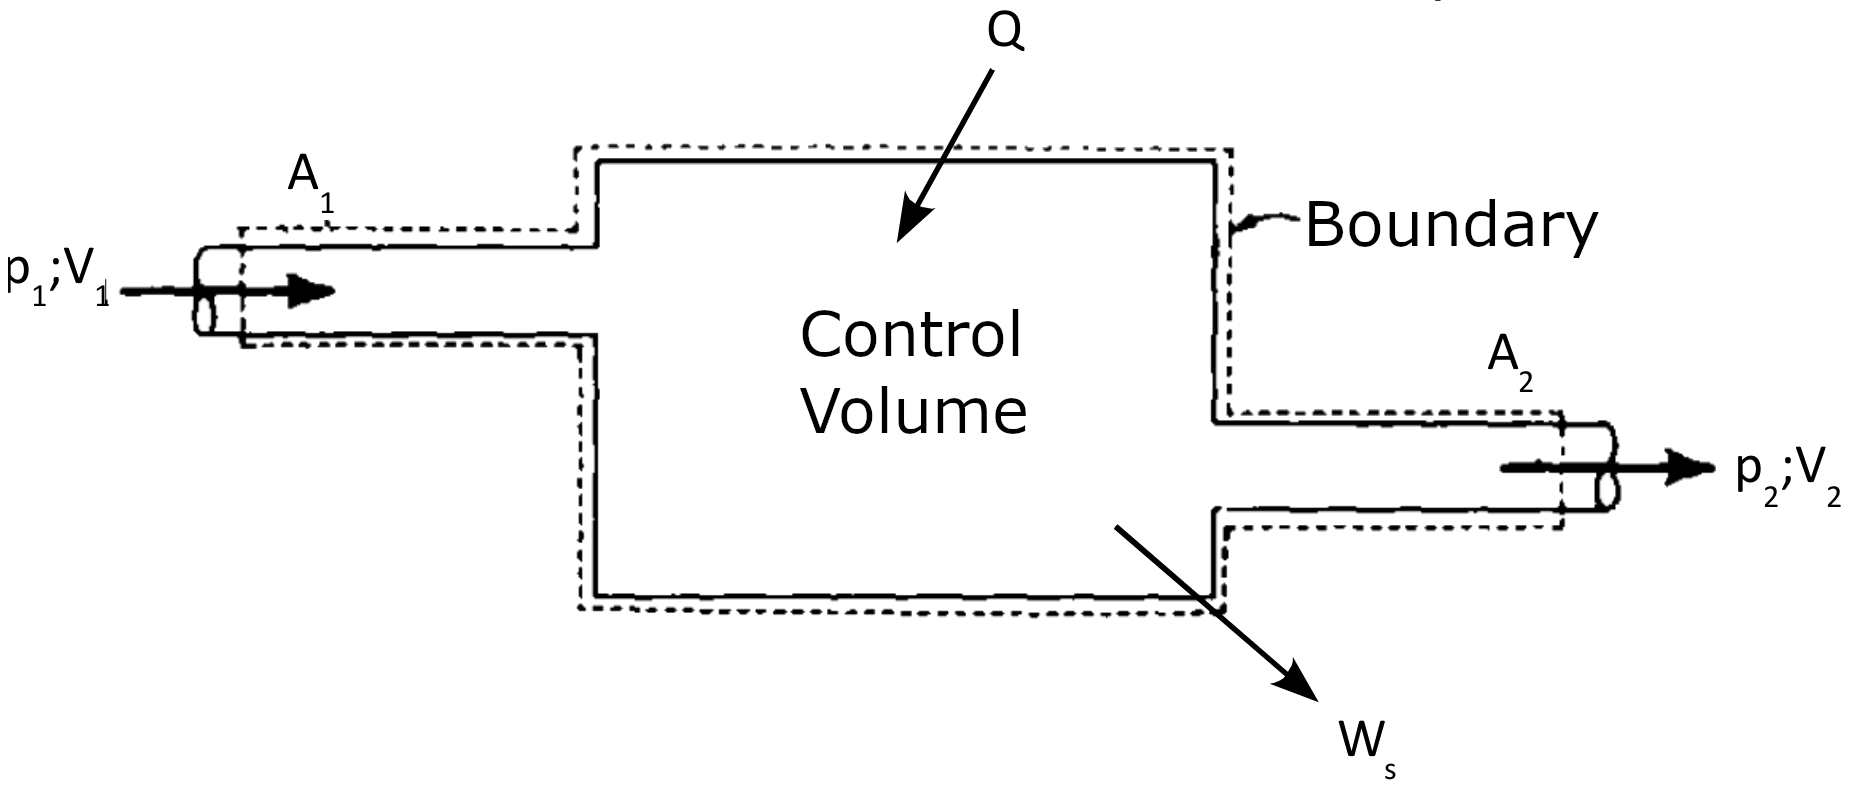
\includegraphics[width=0.7\textwidth]{control_volume.png}
\caption{System control volume \cite{Dewallef2019}.}
\label{fig:C3_VC}
\end{figure}

The Figure \ref{fig:C3_VC} depicts an open system with an entry and exit area $A_1$ and $A_2$ respectively. Posing that the work $W$ is equal to 
\begin{equation}
\setstretch{1}
W = p_2\cdot A_2\cdot v_2\cdot \Delta t - p_1\cdot A_1\cdot v_1\cdot \Delta t + W_s
\end{equation}      
where $P_1$ (resp. $P_2$) and $v_1$ (resp. $v_2$) are the pressure and the velocity at \textbf{1} (resp. \textbf{2}).

By neglecting the variation of the kinetic and potential energy, the energy balance is after some mathematical operations as given in the relation \ref{eq:C3_EBH}
\begin{equation}
\setstretch{1}
q - w_s = u_2 +p_2\cdot \mathrm{v}_2 - u_1 - p_1\cdot \mathrm{v}_1 = h_2 - h_1\label{eq:C3_EBH}
\end{equation}
where $q$, $w_s$, and $h$ are respectively the specific work, heat and \textbf{enthalpy} (in J/kg).  

For the case of an ideal gas, the enthalpy and the internal energy only depend on the temperature $T$. Indeed, taking the relation (\ref{eq:C2_GP}) from the previous chapter, the relation (\ref{eq:C3_h}) can easily be deduced.
\begin{equation}
\setstretch{1}
h = u(T) + p\cdot \mathrm{v} = u(T) + r\cdot T \label{eq:C3_h}
\end{equation}

\subsection{Specific heat}
\quad\ The previous subsection was meant to define the enthalpy. This state variable is used in place of the internal energy when dealing with open system.

An other quantity that is useful for system study is the \textbf{specific heat}. This state variable is defined as the required energy to increase of 1\degree C the temperature of 1kg of a substance. 
 
The required heat to produce this effect depends on the ways the transformation takes place. 
If it is done under constant volume constraint, it is called specific heat at constant volume and denoted $c_v$. 

If the transformation is performed at constant pressure, the symbol associated to the specific heat is $c_p$.
It is worth to note that the specific heat at constant pressure is always higher than the $c_v$. When performing the transformation a constant pressure, the gas expands against the external pressure. This means that the gas does work and, this is the reason behind the greater value of the supplied heat when dealing with a transformation at constant pressure. 

For an ideal gas, the variation of the internal energy can be linked to the specific heat at constant volume as written in the relation (\ref{eq:C3_UC}).

\begin{equation}
\setstretch{1}
du = c_vdT \rightarrow u_2 - u_1 = \int_{T_1}^{T_2} c_vdT\label{eq:C3_UC}
\end{equation} 

Similarly, the variation of the enthalpy can be expressed using the specific at constant pressure.

\begin{equation}
\setstretch{1}
dh = c_pdT \rightarrow h_2 - h_1 = \int_{T_1}^{T_2} c_pdT\label{eq:C3_UP}
\end{equation} 

These two relations, with the equality (\ref{eq:C3_h}), provide the required tools to express the gas constant $r$ as a function of the temperature only. 
\begin{equation}
\setstretch{1}
r = c_p - c_v \label{eq:C3_r}
\end{equation}

Aside the gas constant, the specific heat ratio $k$ (\ref{eq:C3_k}) is also a useful variable to be computed.
\begin{equation}
\setstretch{1}
k = \frac{c_p}{c_v} \label{eq:C3_k}
\end{equation}
\subsection{Carnot cycle}
\quad\, The previous subsections used the first principle of the thermodynamic to deduce two useful state variables, namely the enthalpy and the specific heat.

Now, let's move aside those notions and let consider the case where the transformation applied to a system is reversible. A necessary condition for the reversibility is that the transformation has to be done in quasi-equilibrium. This implies that if the transformation is reversed, the system goes back to its initial state.


\begin{figure}[h]
\centering
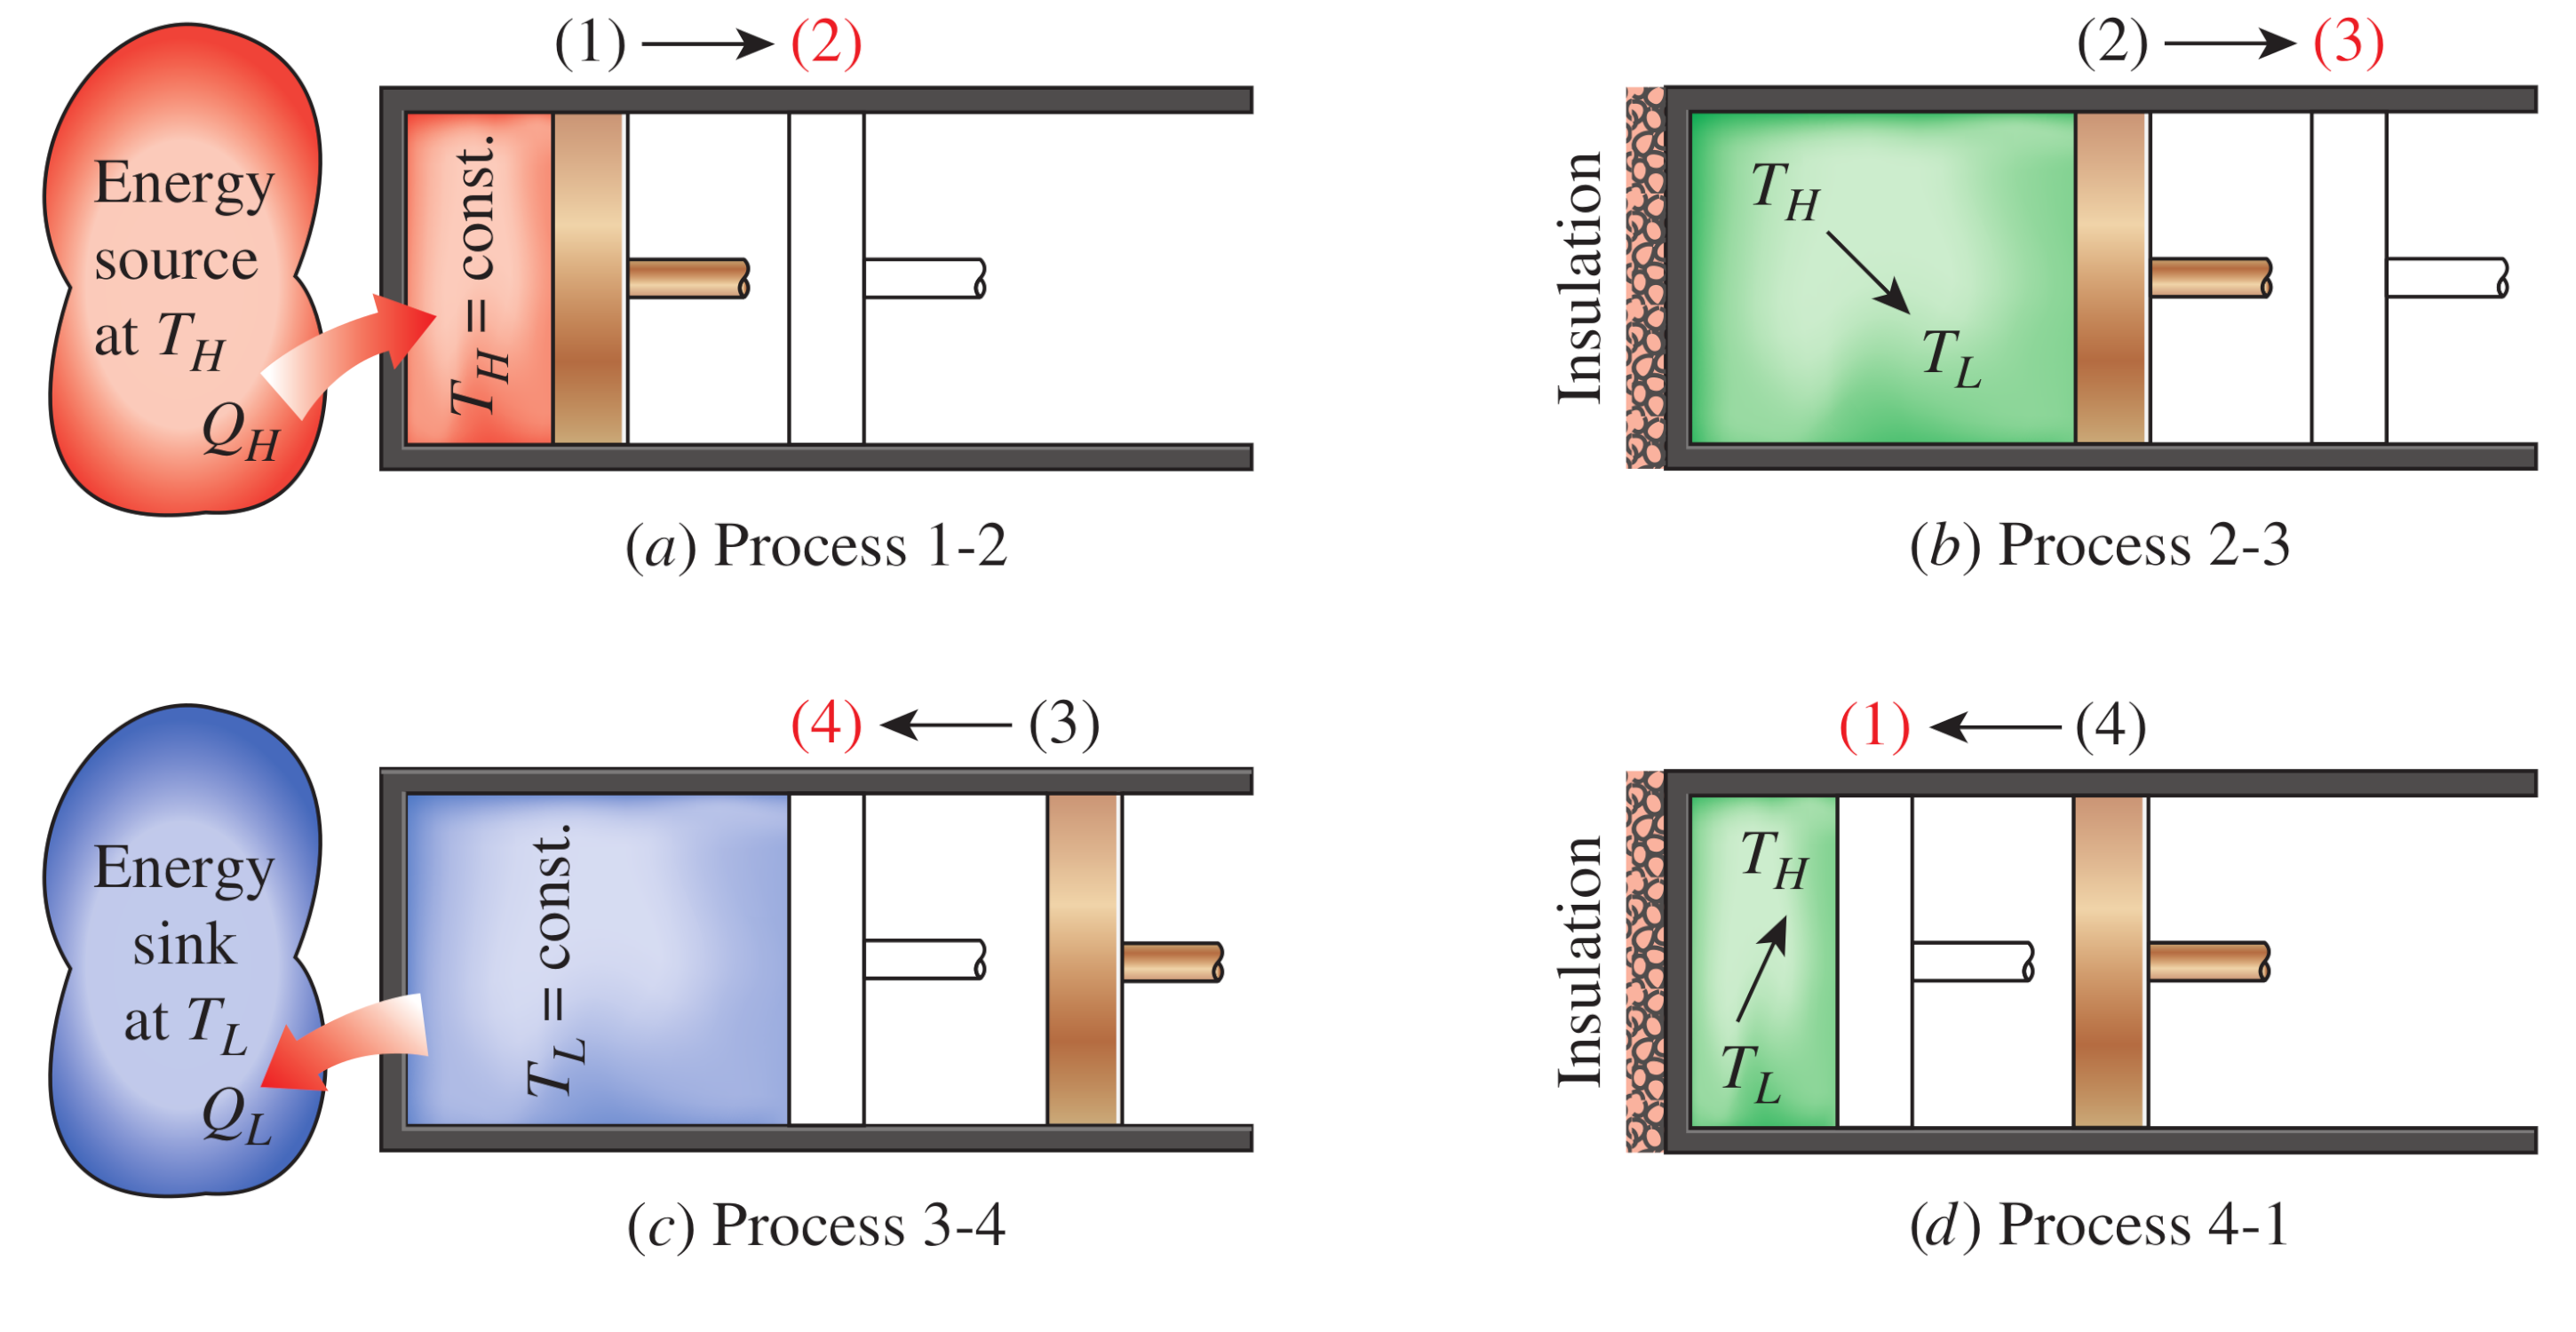
\includegraphics[width=0.7\textwidth]{Carnot_schema.png}
\caption{Carnot cycle - Schematic \cite{2015}.}
\label{fig:C3_Carnot}
\end{figure}
The Carnot cycle is a thermodynamic cycle composed of 4 reversible transformations illustrated on Figure \ref{fig:C3_Carnot}. The transformations are defined as follows.

\begin{itemize}
\setstretch{1}
\item \textbf{1} to \textbf{2} (Figure \ref{fig:C3_Carnot}a): Reversible isothermal expansion with a heat transfer $Q_H$ from the environment to the system
\item \textbf{2} to \textbf{3} (Figure \ref{fig:C3_Carnot}b): Reversible  adiabatic expansion
\item \textbf{3} to \textbf{4} (Figure \ref{fig:C3_Carnot}c): Reversible isothermal compression with a heat transfer $Q_L$ from the system to the environment
\item \textbf{4} to \textbf{1} (Figure \ref{fig:C3_Carnot}d): Reversible adiabatic compression
\end{itemize}

For visual representation, this cycle has been represented in the PV diagram \ref{fig:C3_CarnotPV} where the different transformations are well exposed.
\begin{figure}[h]
\centering
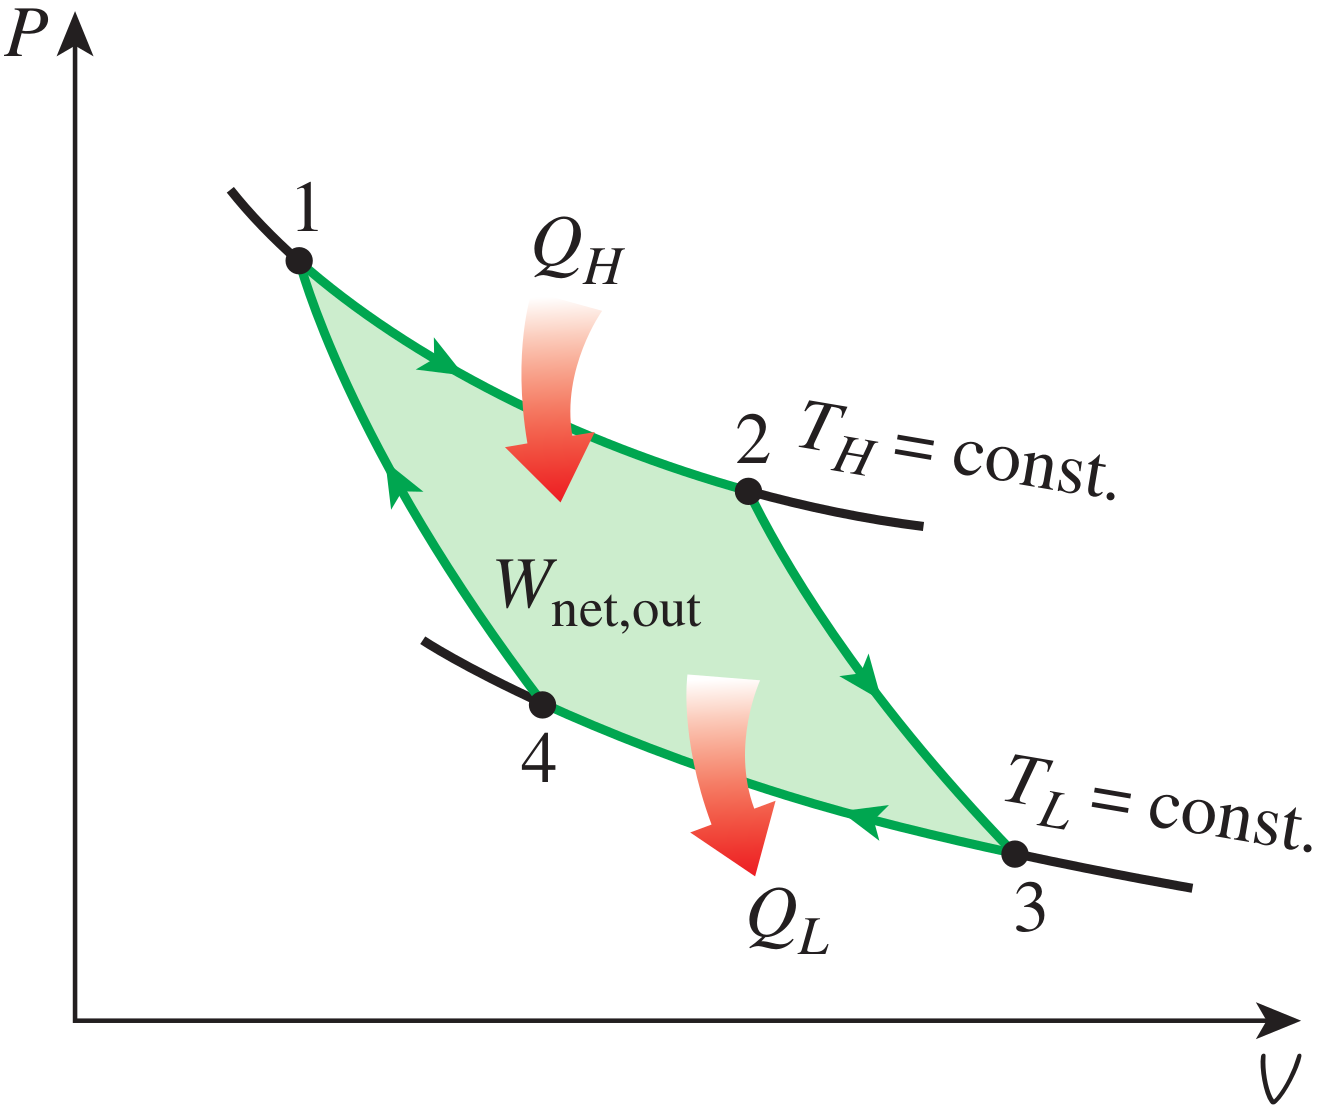
\includegraphics[width=0.5\textwidth]{Carnot_PV.png}
\caption{Carnot cycle - PV diagram \cite{2015}.}
\label{fig:C3_CarnotPV}
\end{figure}

Using the first principle, the net work output is equal to $W_{net,out}=Q_H-Q_L$. This means that the efficiency of the cycle is given by

\begin{equation}
\setstretch{1}
\eta_{carnot} = \frac{W_{net,out}}{Q_H} = 1 - \frac{Q_H}{Q_L}
\end{equation} 

Considering that the working fluid is an ideal gas, it can be demonstrated that the heats $Q_H$ and $Q_L$ can be replaced by the corresponding temperature $T_H$ of the hot source and $T_C$ of the cold sink.

\begin{equation}
\setstretch{1}
\eta_{carnot}=1-\frac{T_H}{T_L}\label{eq:C3_eff_carnot}
\end{equation} 
The efficiency of the Carnot cycle is optimal. This implies that for any system playing with a hot source $T_H$ and a cold sink $T_C$, its efficiency cannot be greater than the Carnot efficiency with the \textbf{same} hot source and cold sink temperatures.

\subsection{Entropy}
\quad\ The last lines explained that a system with a hot source $T_H$ and a cold sink $T_C$ will never have a efficiency greater than the Carnot efficiency (for the same source and sink).

For such cycle, it has been demonstrated in 1865 by the German physician R. J. E. Clausius that "the cyclic integral $\oint\frac{\delta Q}{T}$ is always less than or equal to zero"\cite{2015}.
\begin{equation}
\setstretch{1}
\oint\frac{\delta Q}{T} = \frac{Q_H}{T_H} - \frac{Q_L}{T_L}\leq 0\label{eq:C3_cyc}
\end{equation}

For the Carnot cycle, the integral is equal to zeros because the two ratios $\frac{Q_H}{Q_L}$ and $\frac{T_H}{T_L}$ are equal.

From the definition \ref{eq:C3_cyc} can be defined a new state variable named \textbf{entropy}. The entropy S is always measured based on a reference point and, its expression is given in the relation (\ref{eq:C3_S}).
\begin{equation}
\setstretch{1}
dS \triangleq \frac{\delta Q_{rev}}{T}\label{eq:C3_S}
\end{equation}
where $\delta Q_{rev}$ is the "infinitesimal quantity of heat exchanged in a reversible way between the system and the environment at the temperature T"\cite{Dewallef2019}. 

For a reversible adiabatic transformation, the $\delta Q_{rev}=0$. This implies that the entropy remains constant. Such transformations are called \textbf{isentropic} transformation.
\begin{figure}[h]
\centering
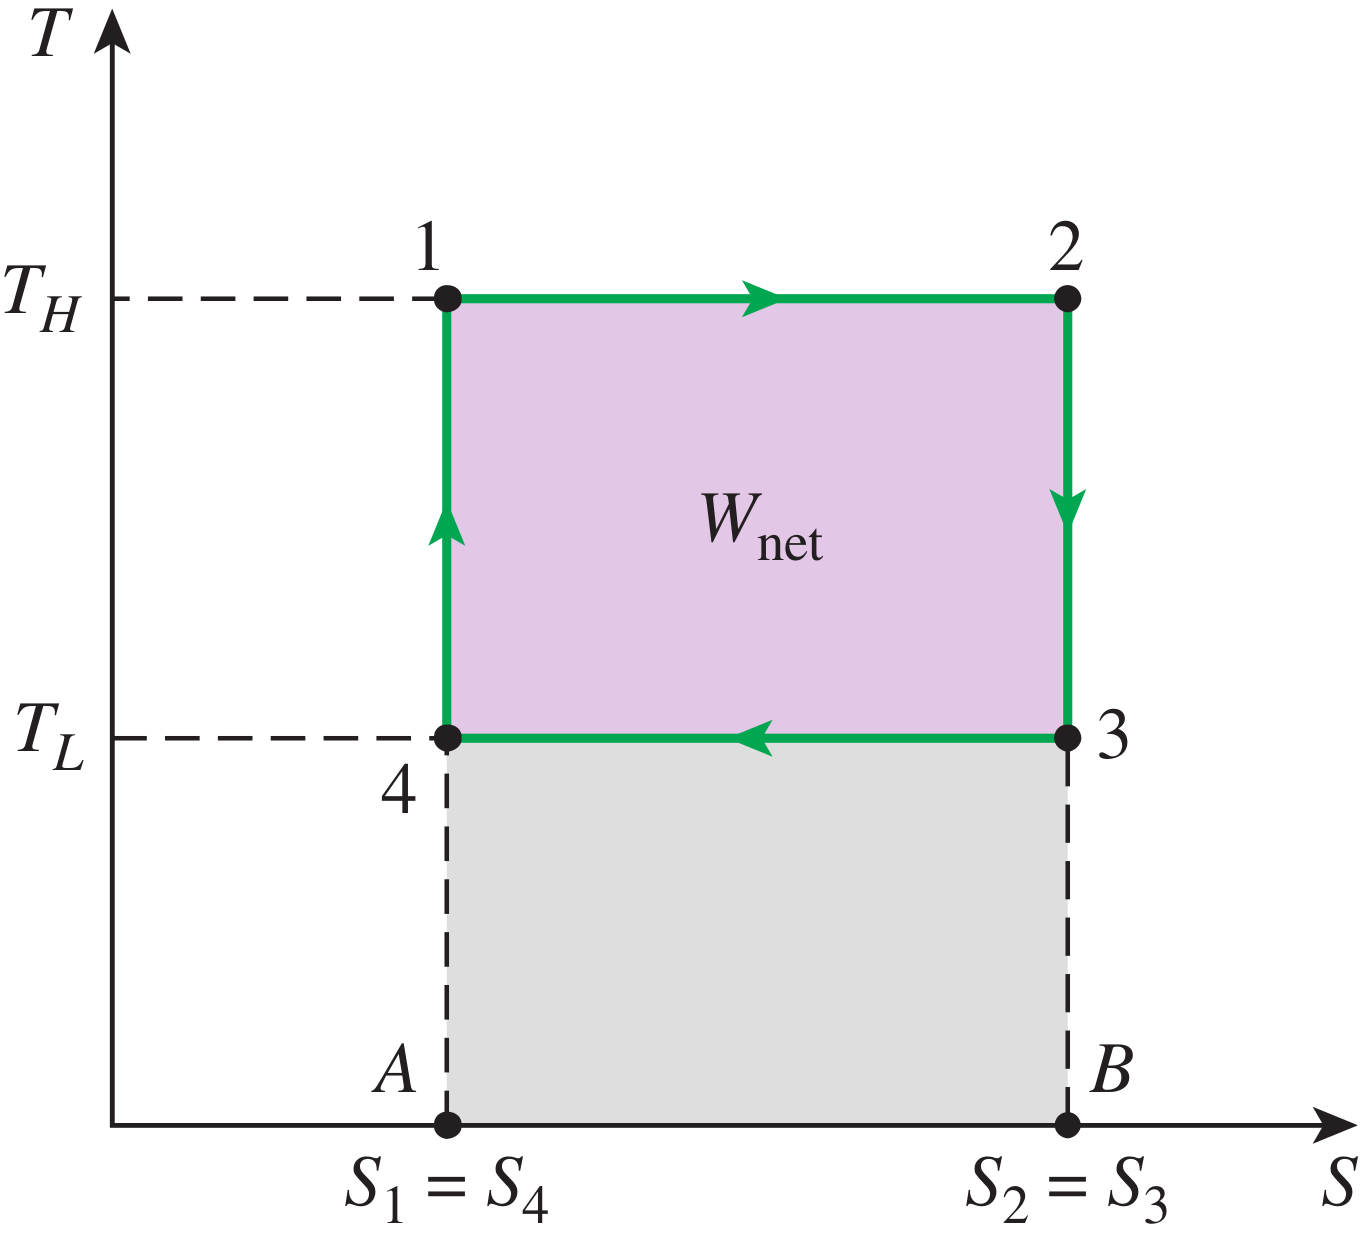
\includegraphics[width=0.5\textwidth]{Carnot_TS.png}
\caption{Carnot cycle - TS diagram \cite{2015}.}
\label{fig:C3_CarnotTS}
\end{figure}
\section{Second principle definition}
\quad\, Defining the entropy gives a great tool to measure the "quality" of the transformation compared to a similar but reversible transformation.

Based on this definition, one formulation of the second principle of the thermodynamic is that for every transformation, the entropy of the final state of any isolated system is greater or equal to the one of the initial state.

Considering the system defined in the previous lines, it can be said that the increase of entropy $\Delta S_L$ of the cold sink have to be at least greater than the diminution of entropy $\Delta S_H$ of the hot source.

In the case of the Carnot cycle, both variations are equal. This is illustrated on the TS diagram \ref{fig:C3_CarnotTS} where the entropy of state \textbf{1} (resp. state \textbf{2}) is the same as the one of state \textbf{4} (resp. state \textbf{3}).

\section{Type of reversible transformations}
\quad\ During this chapter, it has been mentioned several time the notions of reversible processes. 

As it has been explained, a transformation is said reversible if it takes an infinite amount of time to bring the system from its initial state \textbf{1} to its final state \textbf{2}. The different type of transformation are going to be described in the section.

\subsection{Isothermal transformation}
\begin{wrapfigure}{r}{0.3\linewidth}
  \centering
  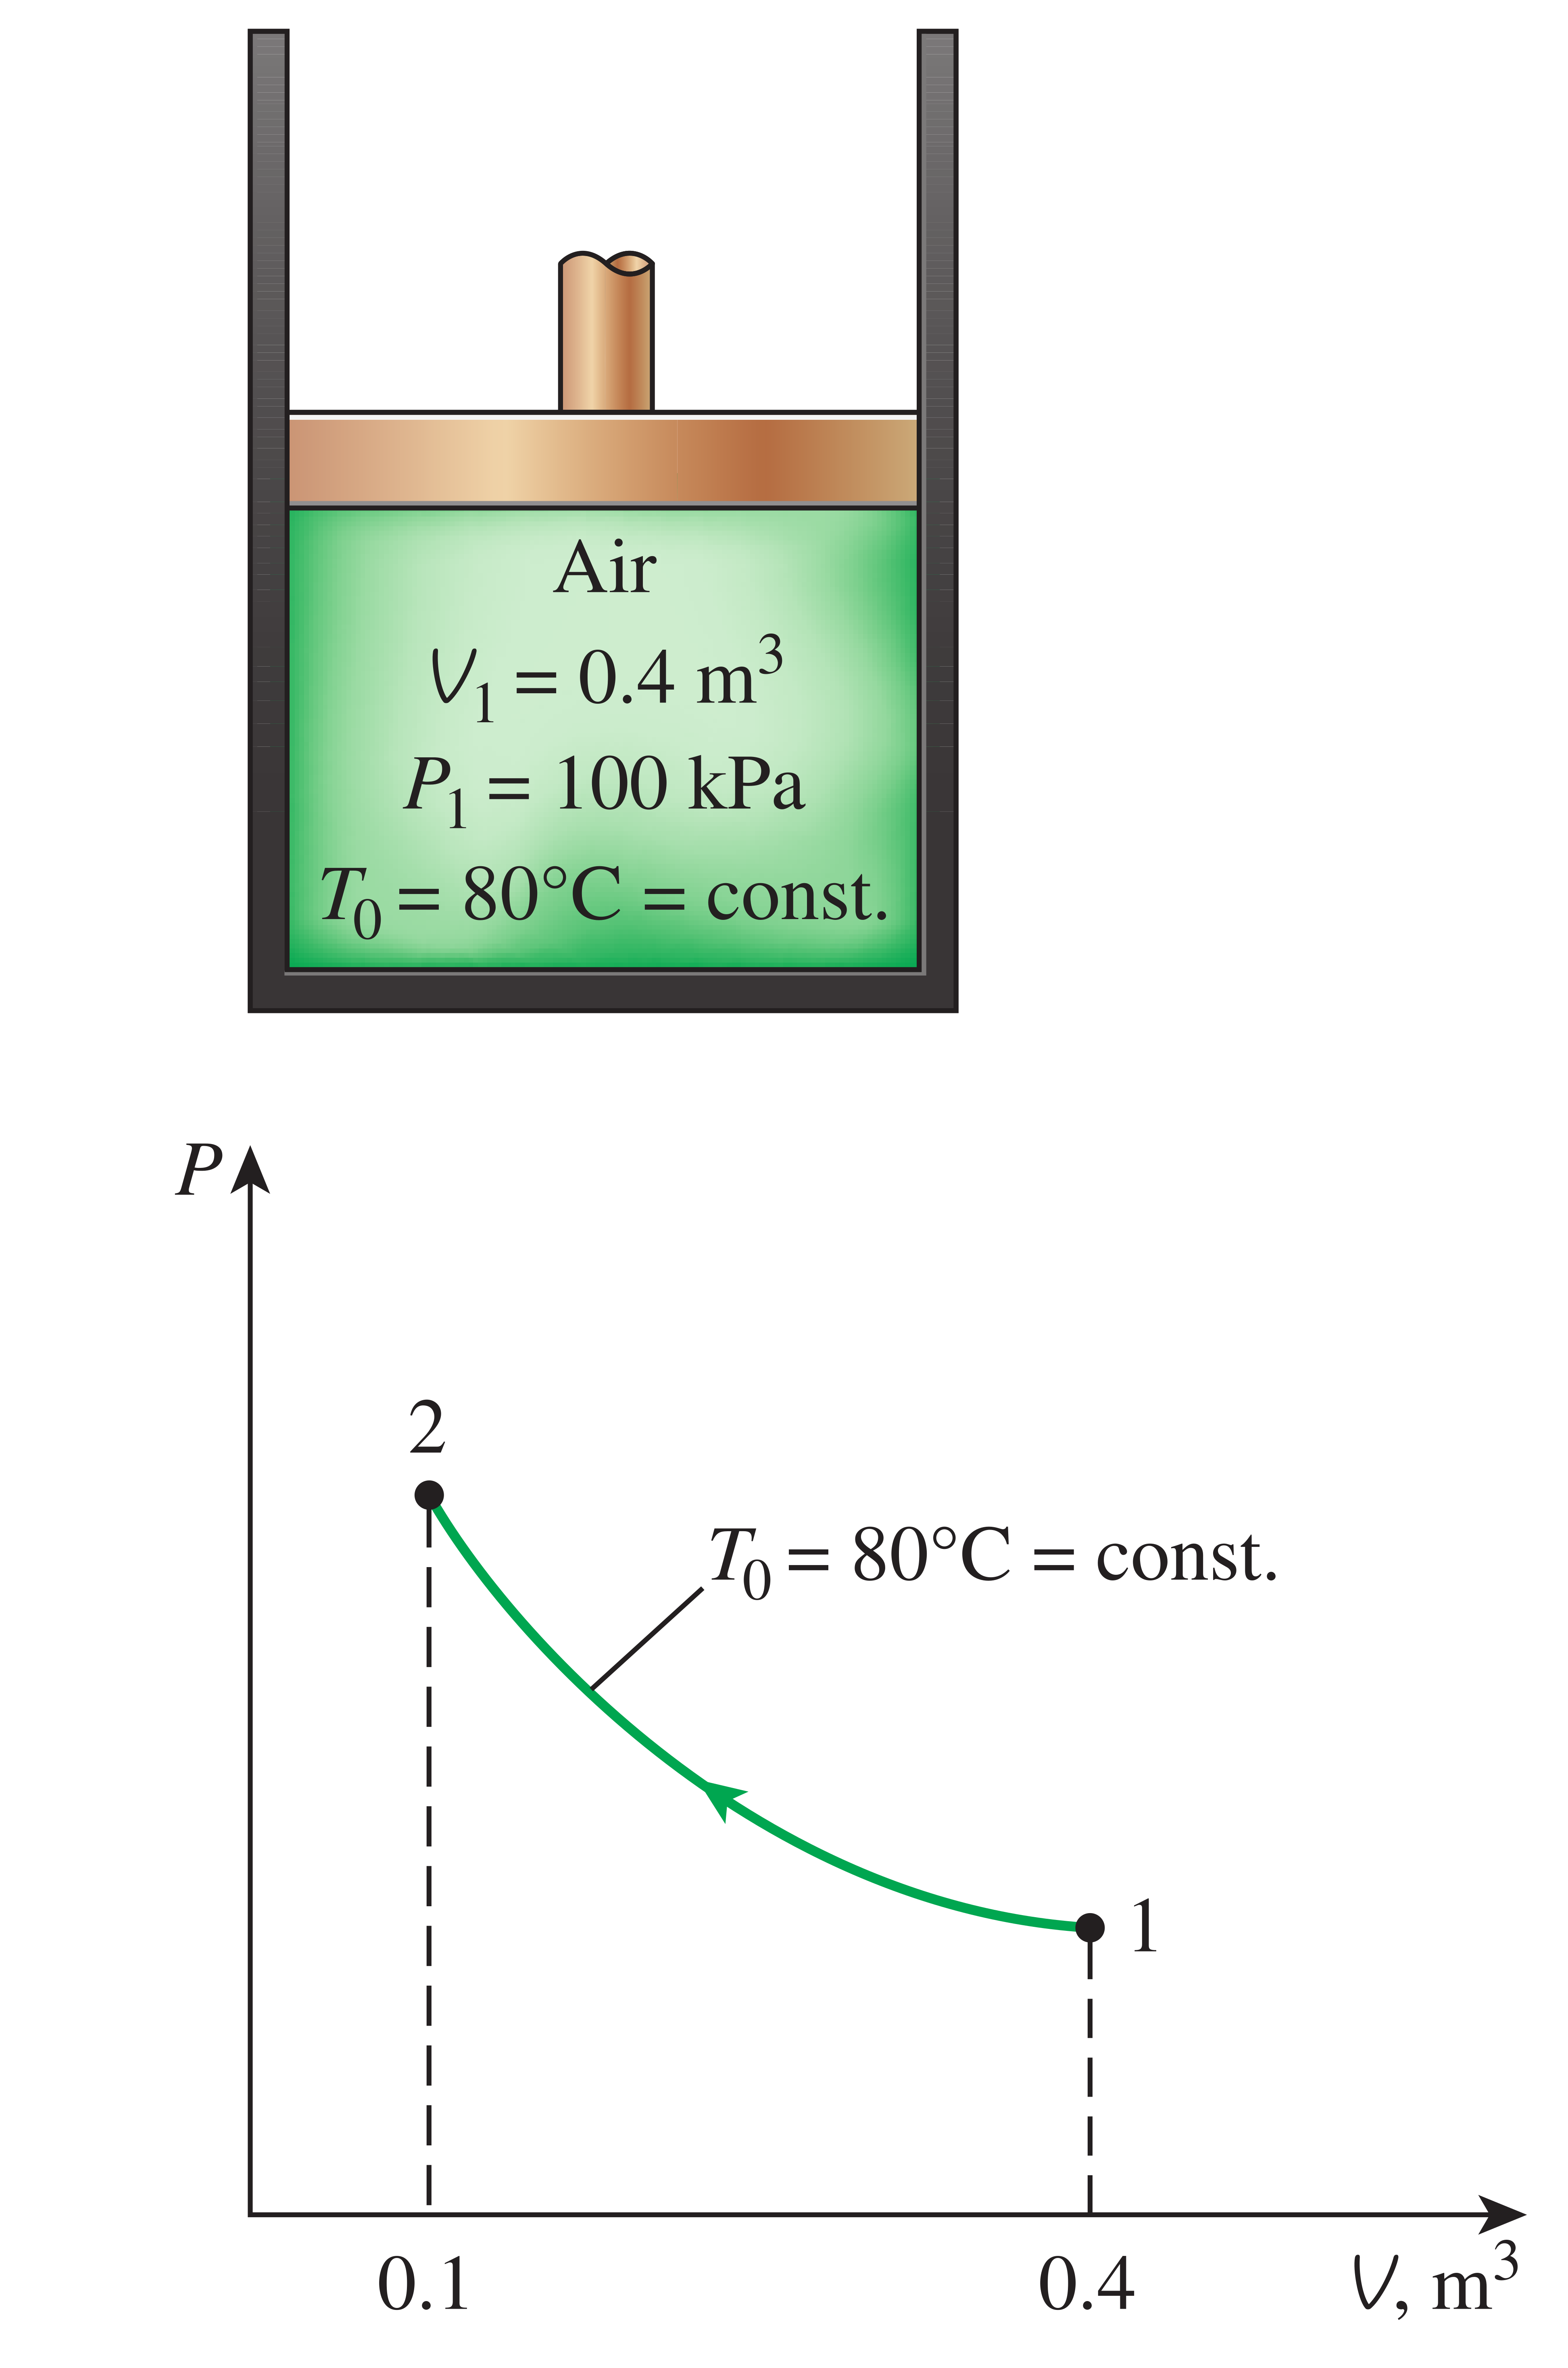
\includegraphics{isoT.png}
  \caption{Isothermal transformation \cite{2015}.}
  \label{fig:C3_isoT}
  \end{wrapfigure}

\quad\ The first type of transformations to be considered are the isothermal processes. Here, considering that the transformation bring the system from state \textbf{1} to \textbf{2}, the equality \(T_2 = T_1\)  is enforced. 

The transformation is said reversible isothermal if during all the process the temperature remains constant. Such transformation is depicted on Figure \ref{fig:C3_isoT}. The ideal gas equation (\ref{eq:C2_GP}) allows to derive the relation (\ref{eq:C3_isoT}) if the mass within the system does not vary.

    \setstretch{1}
  \begin{align}
    p_1\cdot \mathrm{V}_1 &= p_2\cdot \mathrm{V}_2\nonumber\\
    \rightarrow p\cdot \mathrm{V} &= C \label{eq:C3_isoT}  
  \end{align}
  
\setstretch{1.5}
 For a compression (resp. an expansion), the process is said isothermal if the system is cooled (resp. heat up) to bring the final state temperature to its initial value.\clearpage

Considering an isothermal compression, the boundary work $W_b$, corresponding to the area below the curve, is given in the development (\ref{eq:C3_WbisoT})

\begin{wrapfigure}{r}{0.3\linewidth}
  \centering
  \includegraphics{poly.png}
  \caption{Polytropic transformation \cite{2015}.}
  \label{fig:C3_poly}
\end{wrapfigure}

 \setstretch{1}
\begin{align}
  W_b &= \int_1^2 pd\mathrm{V} = C\cdot\int_1^2d\mathrm{V}\nonumber\\
  &= C\cdot \ln \frac{V_2}{V_1} = p_1\cdot V_1\cdot \ln \frac{V_2}{V_1} \label{eq:C3_WbisoT}
\end{align}
\subsection{Polytropic transformation}
 \setstretch{1.5}
\quad\ The polytropic transformation, depicted on Figure \ref{fig:C3_poly}, is  generalization of the isothermal transformation. For an ideal gas, the polytropic transformation is characterized by the relation (\ref{eq:C3_poly}).

  \setstretch{1}
\begin{equation}
  p\cdot \mathrm{V}^n = C \label{eq:C3_poly}
\end{equation}
\setstretch{1.5}
where $n$ is a constant. 

For $n=1$, the transformation simply correspond to the isothermal transformation.
 

\subsection{Isobaric transformation}
\begin{wrapfigure}{l}{0.3\linewidth}
  \centering
  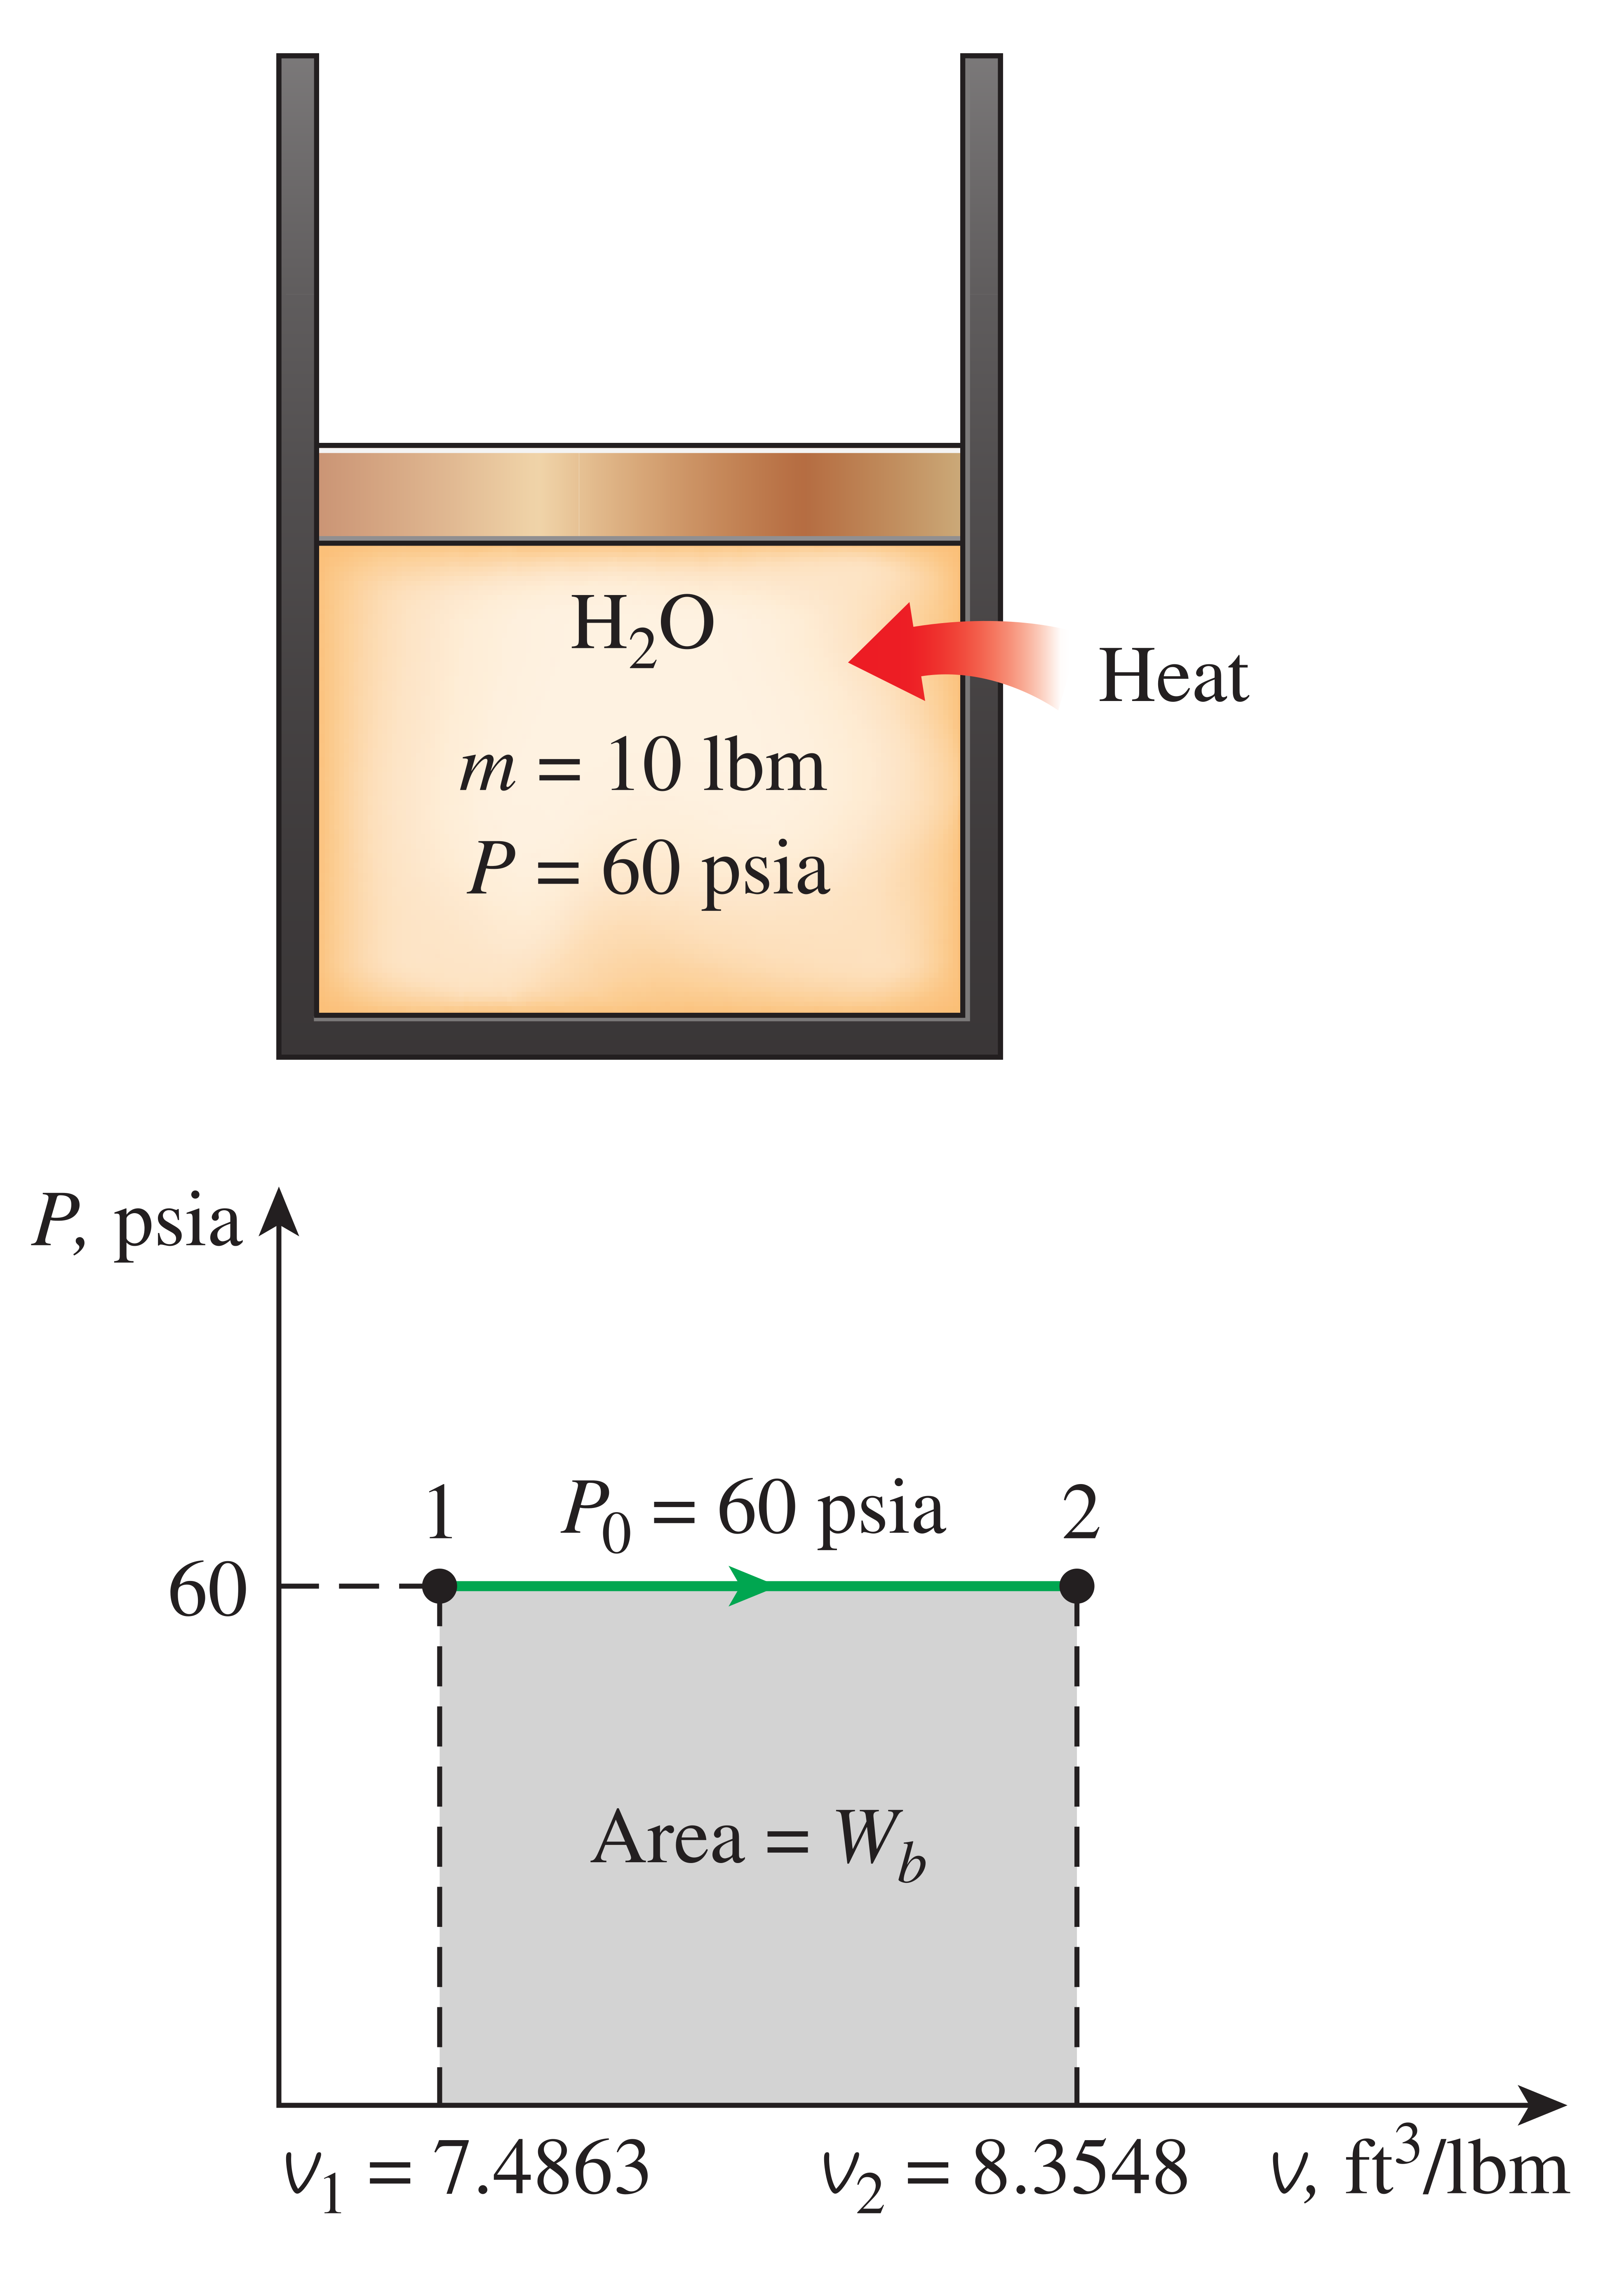
\includegraphics{isoP.png}
  \caption{Isobaric transformation \cite{2015}.}
  \label{fig:C3_isoB}
\end{wrapfigure}

\quad\ The isobaric transformation are one for which the initial and final state are both characterized by the same pressure. Thus, the equality \(p_2 = p_1 = p_0\). Figure \ref{fig:C3_isoB} illustrates such transformation.

Typically, the transformation within the combustion chamber, heat exchanger or piping aim to be as closed as this transformation. Diverging from this ideal transformation implies that the component induces some pressure losses.

As for the isothermal transformation, the boundary work for an isobaric transformation is equal to the area below the curve. Here, the expression is given in the equation (\ref{eq:C3_WbisoP}).

  \setstretch{1}
\begin{align}
  W_b &= p_0\cdot \int_1^2d\mathrm{V}\nonumber\\
   &= p_0\cdot (\mathrm{V_2} - \mathrm{V_1}) = m\cdot p_0\cdot (\mathrm{v_2} - \mathrm{v_1}) \label{eq:C3_WbisoP}
\end{align}\clearpage


\subsection{Isentropic transformation}
\setstretch{1.5}
\quad\ The last transformation to be considered is the isentropic transformation. This transformation corresponds to a reversible adiabatic transformation. 

Typically, when considering the expansion or the compression of a fluid, the manufacturers aim to build a machine which tends to minimize as much as possible the irreversibilities. 

\begin{figure}[h]
  \centering
  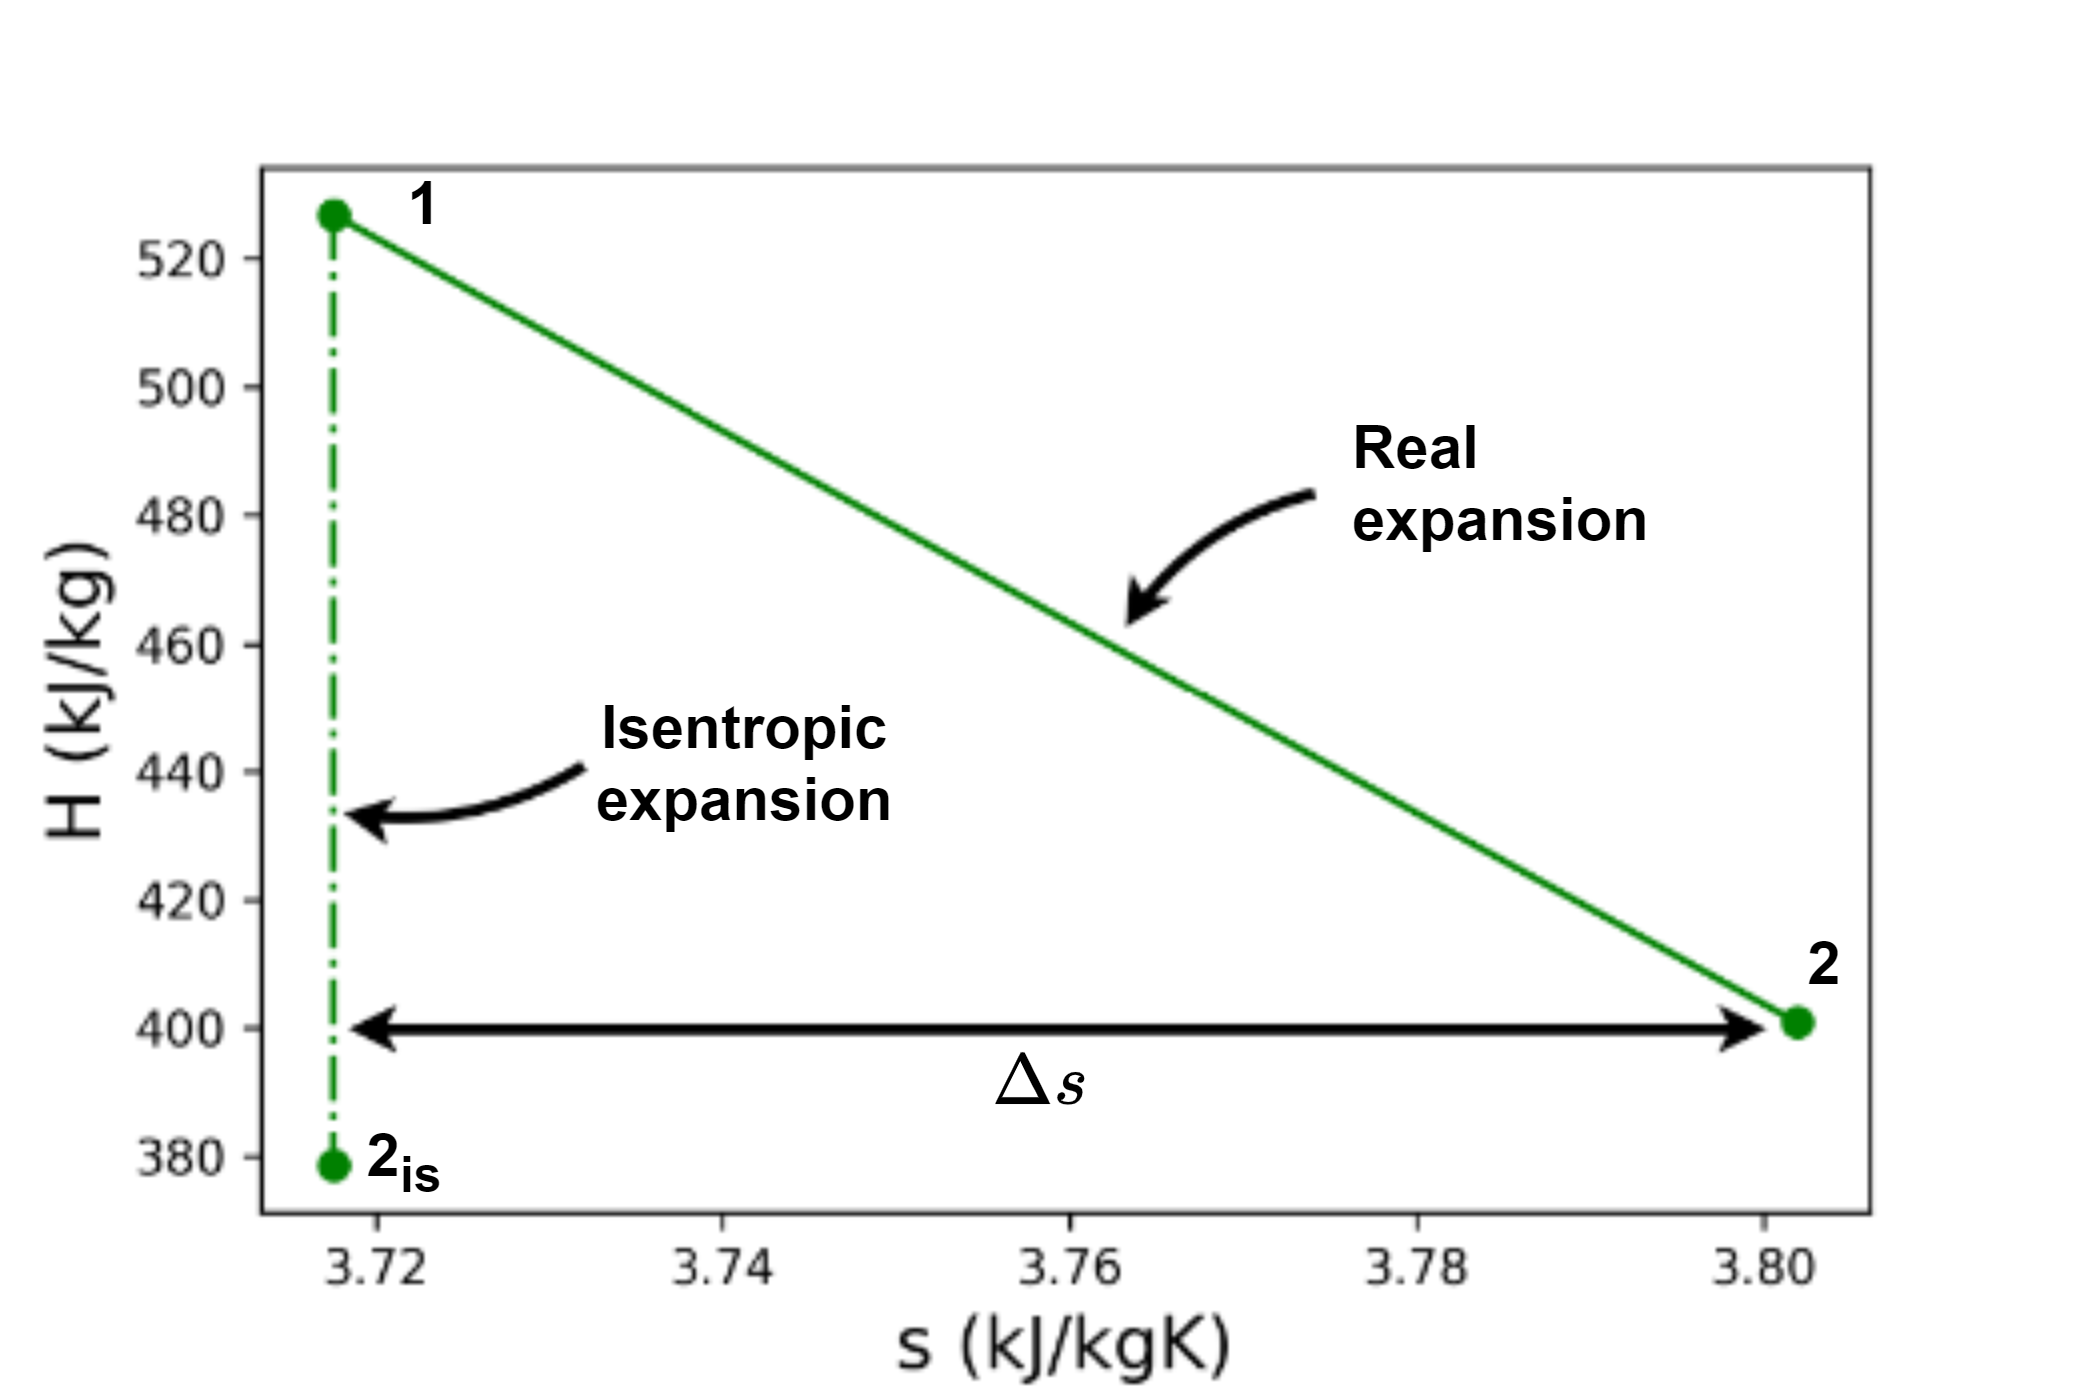
\includegraphics[width=0.6\textwidth]{expansion.png}
  \caption{Isentropic and real expansion.}
  \label{fig:C3_expansion}
\end{figure}

On Figure \ref{fig:C3_expansion} is depicted an isentropic and a real expansion. As it can be noticed, the real expansion produces an augmentation of the entropy of the system. 

Moreover, the isentropic expansion is more efficient since the energy (in term of enthalpy) extracted from the fluid is higher compared to the real expansion. The subscript "is" emphasizing the final state of the isentropic transformation, it can be demonstrated that the enthalpy at the state \textbf{2$_{is}$} is lower than the enthalpy at the state \textbf{2}. The consequence is that more work have been produced during the transformation. 

\section{Computation of the thermodynamic properties}
\quad\, From now, the hypothesis of an ideal gas has been used for the computation of the previously established state variables. However, while this hypothesis remains quite valid when dealing with gas, it cannot be used for a real fluid (e.g. liquid water).

This problem can be solved using the Maxwell relations which provides a linked between the partial derivatives of the state variables $p$, $v$, $T$ and $s$ for a simple compressible system \cite{2015}. 

Those relations can be derived from the four Gibbs relations expressed in (\ref{eq:C3_Gibbs}).

\begin{subequations}
\setstretch{1}
\begin{equation}
  du = Tds - pdv \label{eq:C3_Gibbs1} 
\end{equation}    
\begin{equation}
  dh = Tds + vdp \label{eq:C3_Gibbs2} 
\end{equation}
\begin{equation}
  da = du - Tds - sdT = - pdv - sdT \label{eq:C3_Gibbs3} 
\end{equation}    
\begin{equation}
  dg = dh - Tds - sdT = vdp - sdT \label{eq:C3_Gibbs4}
\end{equation} \label{eq:C3_Gibbs}
\end{subequations}

where the state variables $a$ and $g$ are the Helmholtz and Gibbs function (respectively).

Analyzing the relations allows to notice that each of them are of the form
\begin{align}
\setstretch{1}
dz &= Mdx + Ndy\label{eq:C3_Maxbase}\\
\text{with } \left.\frac{\partial M}{\partial y}\right|_x &= \left.\frac{\partial N}{\partial x}\right|_y\label{eq:C3_partMax}
\end{align}

Using this property, the links between the different state variables are easily obtained by applying the relation (\ref{eq:C3_partMax}) to the equations (\ref{eq:C3_Gibbs1}) to (\ref{eq:C3_Gibbs4}).
\begin{subequations}
\setstretch{1}
\begin{equation}
  \left.\frac{\partial T}{\partial v}\right|_s =  - \left.\frac{\partial p}{\partial s}\right|_v \label{eq:C3_Max1} 
\end{equation}    
\begin{equation}
  \left.\frac{\partial T}{\partial p}\right|_s = \left.\frac{\partial v}{\partial s}\right|_p \label{eq:C3_Max2}  
\end{equation}
\begin{equation}
  \left.\frac{\partial s}{\partial v}\right|_T = \left.\frac{\partial p}{\partial T}\right|_v \label{eq:C3_Max3} 
\end{equation}    
\begin{equation}
  \left.\frac{\partial s}{\partial p}\right|_T =  - \left.\frac{\partial v}{\partial T}\right|_p \label{eq:C3_Max4} 
\end{equation} \label{eq:C3_Max}
\end{subequations}

The relations (\ref{eq:C3_Max}) are called Maxwell equations are helpful in thermodynamics. They provide a method to calculate the variation of the entropy of a system based on the measurement of the variation of the pressure, volume and temperature.

However, this method for calculating the thermodynamic variables is limited to simple compressible system and cannot be used when the system involves "electrical, magnetic, and other effects"\cite{2015}.

These are the relations used when using a digital library for the thermodynamic assessment of the state of a pure fluid with real properties. The open-source library named \textbf{CoolProp}\cite{Bell2014} is one of the best known and. In this work, the library will be called many time when the ideal gas approximation is not relevant.

\section{Entropy variation}
\quad\, The previous section introduced the four equations of state (\ref{eq:C3_Gibbs1}) to (\ref{eq:C3_Gibbs4}). Among those, the second equation allows to write the relation (\ref{eq:C3_ds})
\begin{equation}
ds = c_p\frac{dT}{T} - r\frac{dp}{p}\label{eq:C3_ds}
\end{equation}
using the definition (\ref{eq:C3_UP}) of the enthalpy variation and the ideal gas equation (\ref{eq:C2_GP}).

Performing the integration over the path of a transformation going from state \textbf{1} to state \textbf{2}, it can be obtained 
\begin{equation}
s_2 - s_1  = \int_1^2\frac{c_p}{T}dT - r\cdot ln\frac{p_2}{p_1}
\end{equation}
If it is supposed that the variation of the specific heat with respect to temperature are negligible, it can be written
\begin{equation}
s_2 - s_1= r\cdot \left(\frac{k}{k-1}\cdot ln\frac{T_2}{p_1} - ln\frac{p_2}{p_1}\right) = r\cdot ln\left[\frac{p_1}{p_2}\cdot\left(\frac{T_2}{T_1}\right)^\frac{k}{k-1}\right] \label{eq:C3_Deltas}
\end{equation}
where the $c_p=\frac{r\cdot k}{k-1}$ by using the two relations (\ref{eq:C3_r}) and (\ref{eq:C3_k}).

For an isentropic process, the equality $s_2=s_1$ is enforced. Thus, the following relationships can be derived.

\begin{subequations}
\setstretch{1}
\begin{equation}
\frac{p_2}{p_1} = \left(\frac{T_2}{T_1}\right)^\frac{k}{k-1}\label{eq:C3_isrelPT}
\end{equation}
\begin{equation}
\frac{\rho_2}{\rho_1} = \left(\frac{T_2}{T_1}\right)^\frac{1}{k-1}
\label{eq:C3_isrelrhoT}
\end{equation}
\label{eq:C3_isrel}
\end{subequations}

\section{Isentropic efficiency} \label{C3:Isen_eff}
\quad\, For any real transformations, there is always an augmentation of the entropy when the system goes from its initial state \textbf{1} to its final state \textbf{2}. This implies that the difference $s_2 - s_1$ is greater than zero.

This can be characterized by defining the isentropic efficiency as being the image of the irreversibilities induced by the transformation. this type of efficiency is very frequently used when studying the compression or the expansion of a fluid.

For a compression or an expansion, the isentropic efficiency is defined by stating that the pressure ratio $\frac{p_1}{p_2}$ is the identical for both the isentropic and non isentropic transformation. Let's substituting this ratio by the constant $\Pi$. 

Considering first the ideal case, the relation (\ref{eq:C3_isrelPT}) gives
\begin{equation}
T_{2,is} = T_1\cdot\Pi^\frac{k-1}{k}
\end{equation}

Then, for the real transformation, the left-hand-side of the relation (\ref{eq:C3_Deltas}) is greater than zero. This implies that
\begin{equation}
T_{2} > T_{2,is} = T_1\cdot\Pi^\frac{k-1}{k}
\end{equation}

As can be noticed, the real transformation leads to a final state temperature bigger than for the isentropic transformation. This difference allows to define the isentropic efficiency $\eta_{is}$. The definition varies based on the desired transformation
\begin{itemize}
\setstretch{1}
\item Compression: $\eta_{is}=\frac{T_{2,is}-T_1}{T_2-T_1}=\frac{h_{2,is}-h_1}{h_2-h_1}$
\item Expansion: $\eta_{is}=\frac{T_1-T_{2}}{T_1-T_{2,is}}=\frac{h_1-h_{2}}{h_1-h_{2,is}}$
\end{itemize}
where the temperature and the enthalpy variation provide the same output result due to the ideal gas hypothesis. For real fluid, the only valid definition of the isentropic efficiency is the one based on the enthalpy variation. 
\newpage
%%%%%%%%%%%%%%%%%%%%%%%%%%%%%%%%%
%% Chapitre 4:                 %%
%% Brayton_cycle               %%
%%%%%%%%%%%%%%%%%%%%%%%%%%%%%%%%%
\graphicspath{{Chapitre_4/Images/}}
\chapter{Thermodynamic components}\label{C4}
%%%%%%%%%%%%%%%%%%%%%%%%%%%%%%%%%%%
%%%%%                         %%%%%
%%%%% Introduction chapitre 3 %%%%%
%%%%%                         %%%%%
%%%%%%%%%%%%%%%%%%%%%%%%%%%%%%%%%%%
\quad\ In the beginning of the previous chapter, it has been mention that the Brayton cycle composed of several components that are more or less complex. The behavior of these components, which is required to realize the study the global system, is based on the thermodynamic notions that have been introduced all along the past lines.

This chapter will be focused on the description of those components. For each of them, it will be provided the concepts or principles that will be used during this work. Then, a description of the Brayton cycle itself will be provided. Different configurations will be proposed and compared.
\section{Turbomachines}
%%%%%%%%%%%%%%%%%%%%%%%%%%%%%%%%%%%
%%%%%                         %%%%%
%%%%%    <<Turbomachines>>    %%%%%
%%%%%                         %%%%%
%%%%%%%%%%%%%%%%%%%%%%%%%%%%%%%%%%%
\quad\ The first family of components to be studied is the turbomachines. The machines owning to this family are ones “that exchange energy between the
fluid traversing it and mechanical energy supplied to or extracted from the machine” \cite{Hillewaert2019}. Those machines are \textbf{rotating} machines
can be categorized into two families.

The first family of turbomachines are turbomachines which inject or extract energy from an incompressible flow. These transformations on the fluid  are respectively performed by pumps and hydraulic turbines.

The second family are turbomachines dealing with compressible flow. Here, some extract effects are taken into account. For instance, the velocity of the flow can be at some points limited due to choking effects. Also, since the flow is compressible its density can vary along the path, the velocity will varies along the path as well. These effects will be rediscussed in a future part of this section.

Turbomachines that are encompassed in this second category are compressors and gas turbines. As for the pumps and hydraulic turbines, compressors and turbines aim to inject and extract energy into/from the flow.

\subsection{General principles}
\quad\ Some principles used when designing incompressible and compressible flow based machines are common for both of these families. Among these principles, it can be emphasized the velocity triangle, the enthalpy and rhotalpy conservation, and the similarity analysis. The two first provides tools to well design the blades of the turbomachines, while the other principle is used to derive the performance of a given machines based on non-dimensional quantities. The following lines will explain the basis about these different principles. 

\subsubsection{Velocity triangle}
\quad\ When considering the rotating part of the turbomachine (named rotor), there is, in addition to the absolute frame of reference, a rotating frame which is attached to the rotor. This leads to definition of three components for the velocity of the fluid: 

\begin{itemize}
    \item Absolute velocity \(\mathbf{v}\): velocity of the fluid in the absolute frame (\(\mathbf{x},\mathbf{y}\)).
    \item Rotating speed of the rotor \(\mathbf{u_r}\): rotating speed of the rotor in the absolute frame (\(\mathbf{x},\mathbf{y}\)).
    \item Relative velocity \(\mathbf{w_r}\): velocity of the fluid in the relative frame  (\(\mathbf{x'},\mathbf{y'}\)).
\end{itemize}

\begin{figure}[h]
    \centering
    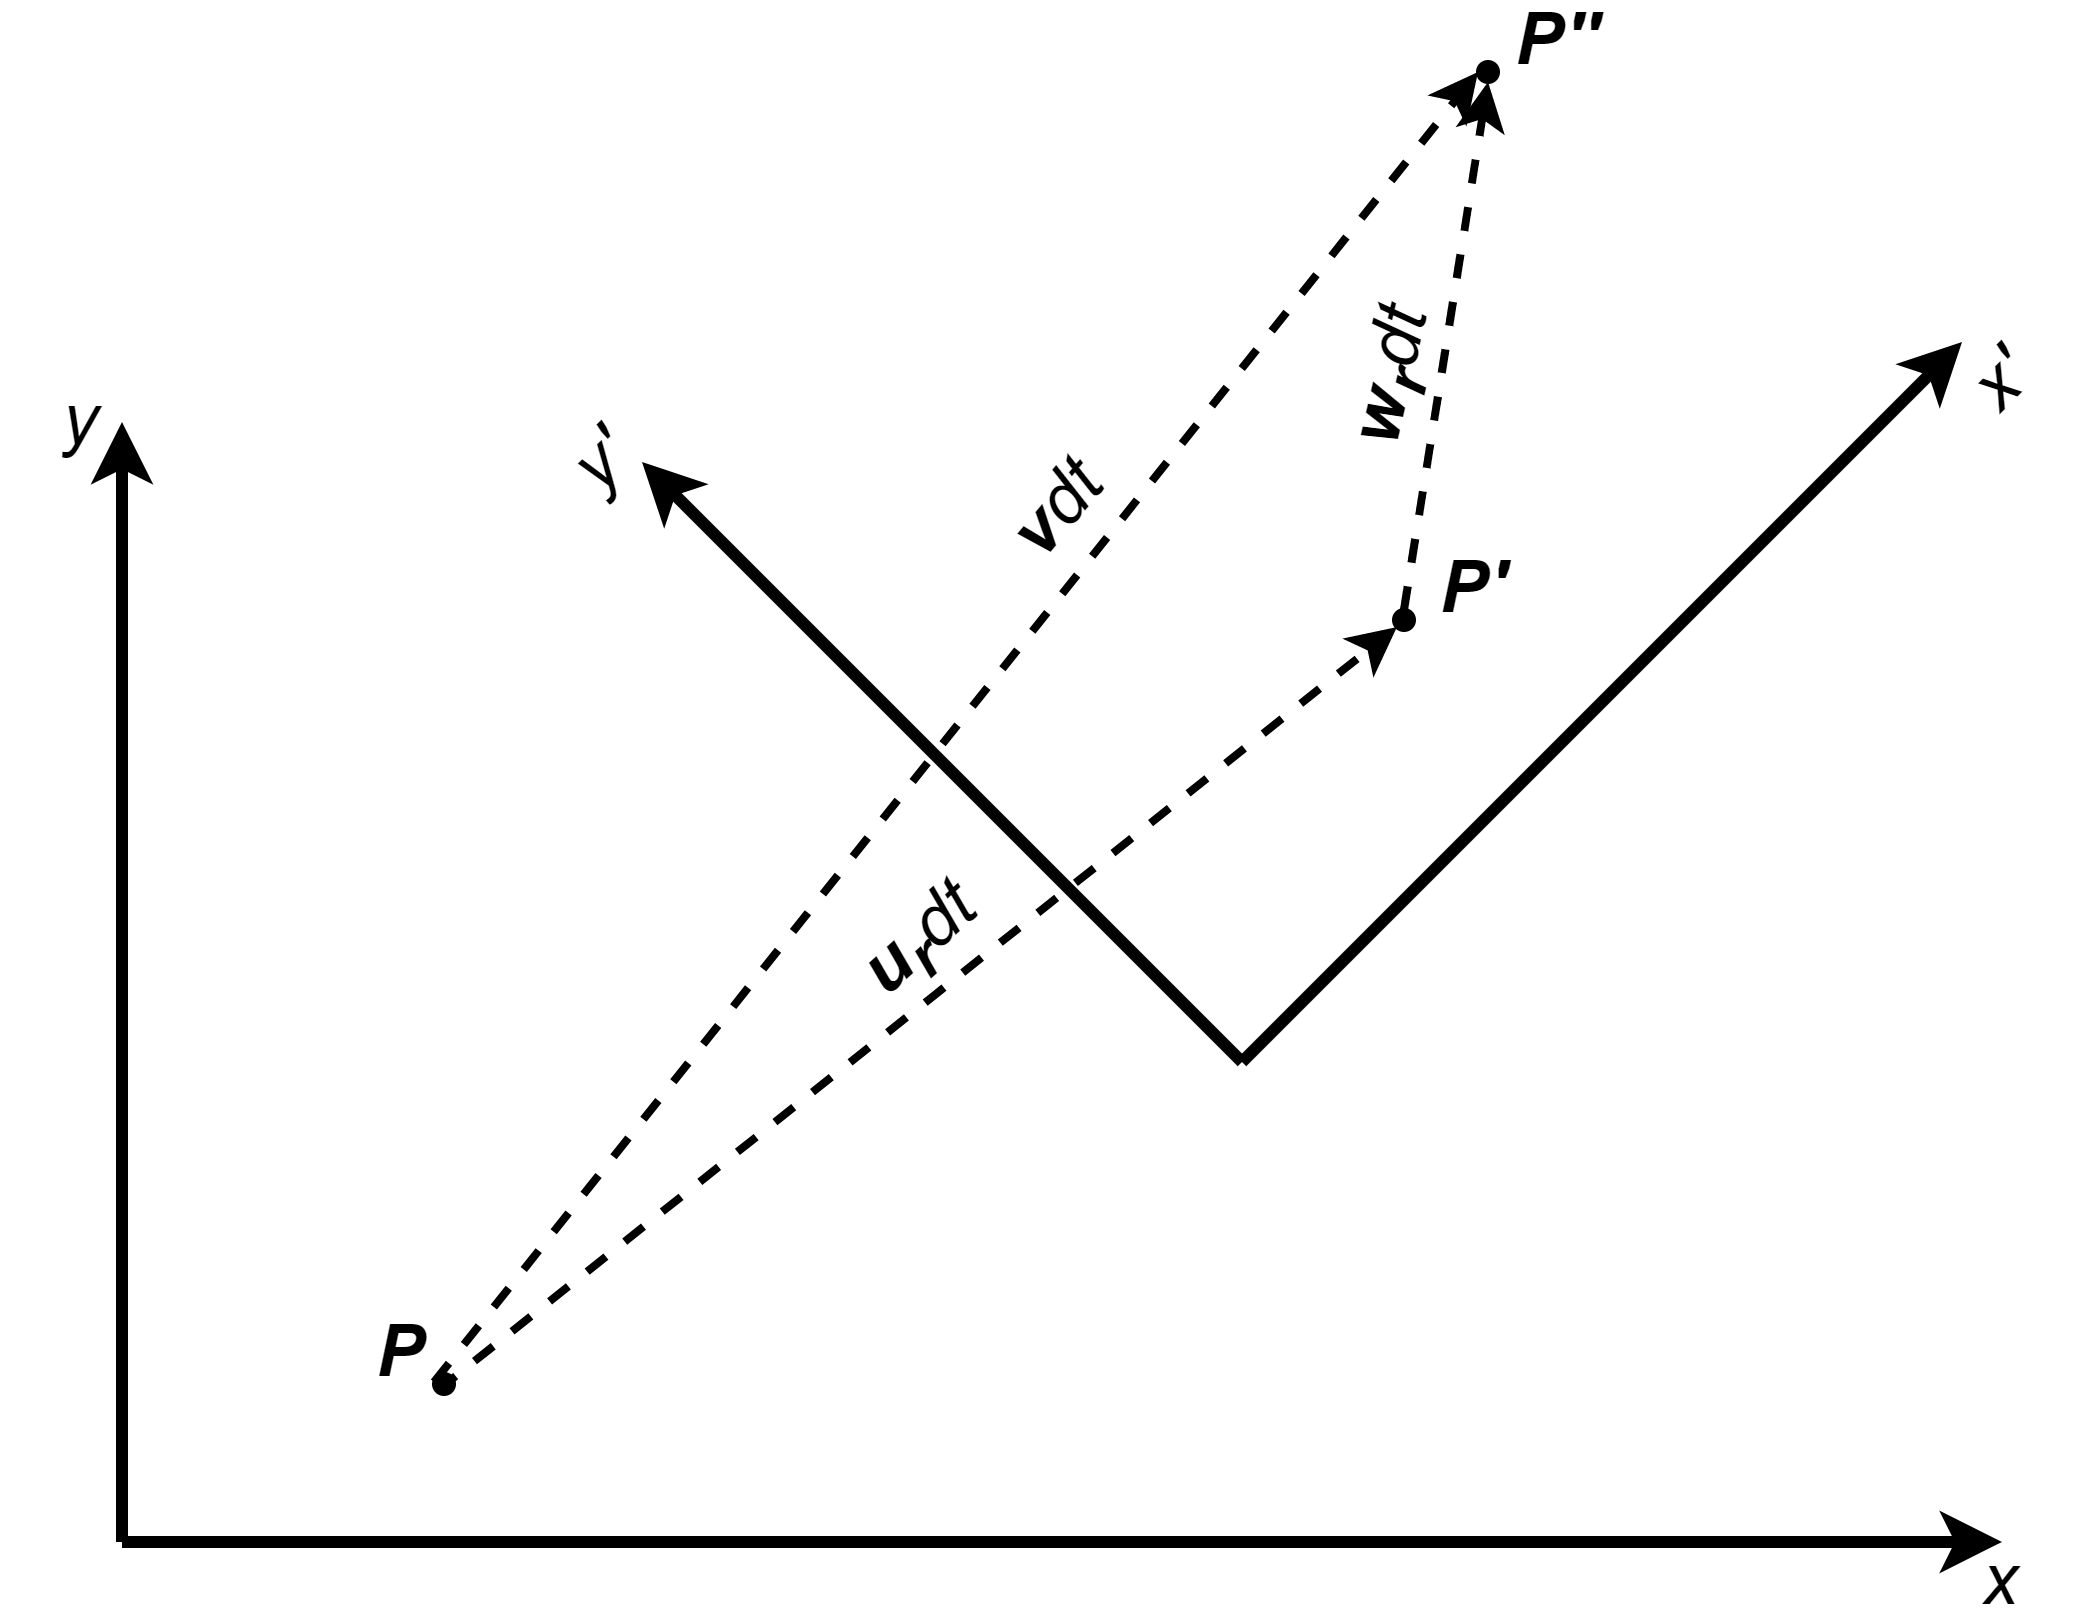
\includegraphics[width=0.6\textwidth]{Frames.png}
    \caption{Absolute and rotating frames.}
    \label{fig:C4_frames}
\end{figure}

Figure \ref{fig:C4_frames} shows the representations in the space of these different definitions of the velocity. Considering a point at $P$ in the time t=0, this point is moving to \(P''\) in the time t=dt.  
The drawing shows that the following equality (\ref{eq:C4_velocity}) is enforced at any time.

\begin{equation}
    \setstretch{1}
    \mathbf{v} = \mathbf{u_r} + \mathbf{w_r} \label{eq:C4_velocity}
\end{equation}

Another way of representations of these velocities is to draw the velocity triangle. The velocity triangle is defined as depicted on Figure \ref{fig:C4_vtriang}.

\begin{figure}[h]
    \centering
    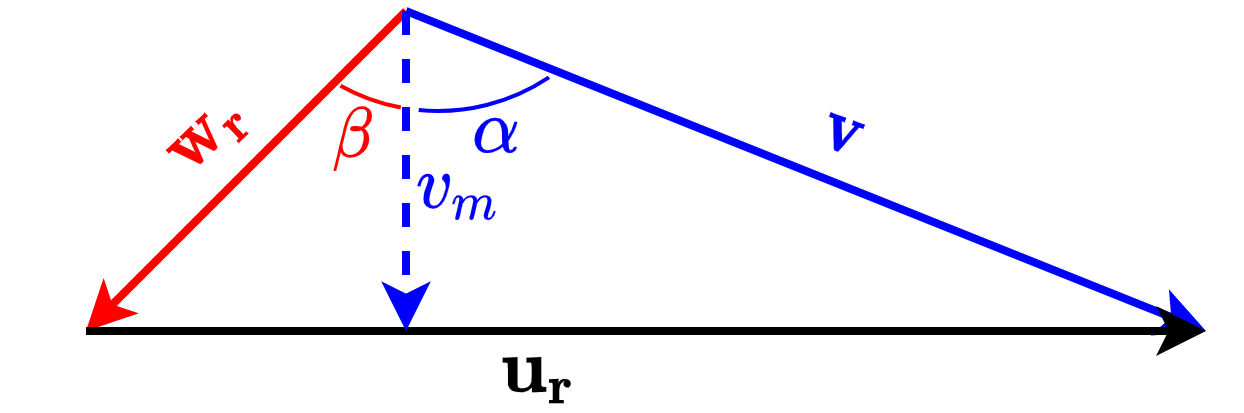
\includegraphics[width=0.6\textwidth]{Vtriangle.png}
    \caption{Velocity triangle.}
    \label{fig:C4_vtriang}
\end{figure}
where $v_m$ is the projection of the vector $\mathbf{v}$ on the meridional axis.

Here, two angles $\alpha$ and $\beta$, respectively the absolute and relative flow angles, can be defined. Those angles will allow to design the shape of the rotating blade based on the desired applications. 

\subsubsection{Enthalpy and rhothalpy conservation}
\quad\ It has been mentioned before that, for a compressible flow, the velocity can vary along the path. The notion of static and total (or stagnation) quantities have been established to take into account this variation of velocity. Stagnation quantities will be identified by the superscript ''0''.

For instance, the total enthalpy is given by
\begin{equation}
    \setstretch{1}
    h^0 = h + \frac{1}{2}\cdot v^2\label{eq:C4_h0}
\end{equation}

Now, considering an adiabatic transformation without viscous work, the total enthalpy is conserved between the initial state and the final state.
\begin{equation}
    \dot{m}_1\cdot h_1^0 = \dot{m}_2 h_2^0 \label{eq:C4_hcons}
\end{equation}
which can be reduced to \(h_1^0 = h_2^0\) if we supposed that the transformation is performed without any leakages (\(\dot{m}_1=\dot{m}_2\)). The states \(1\) and \(2\) are associated to the orthogonal boundaries to the flow of the selected control volume delimiting the studied system.

\begin{equation}
    \setstretch{1}
    i^0 = h + \frac{1}{2}\cdot w_r^2 - \frac{1}{2}\cdot u_r^2 \label{eq:C4_i0}
\end{equation}

Similarly, using the definition (\ref{eq:C4_i0}) of the stagnation rhotalpy, it is obtained from the Euler equation (\ref{eq:C4_Euler}) that, within a rotor, the total rothalpy is conserved through the transformation process.

\begin{align}
    \setstretch{1}
    h_2^0 - h_1^0 = \frac{1}{2}\cdot & \left(v_2^2 - v_1^2\right) - \frac{1}{2}\cdot \left(w_{r,2}^2 - wr_{r,1}^2\right) + \frac{1}{2}\cdot \left(u_{r,2}^2 - u_{r,1}^2\right)\label{eq:C4_Euler} \\
    \text{with }                     & v = \left|\vect{v}\right|\quad\text{;}\quad  w_r = \left|\vect{w_r}\right|\quad\text{;}\quad u_r= \left|\vect{u_r}\right|\nonumber
\end{align}

The rhotalpy conservation is then expressed as stated in the equality (\ref{eq:C4_icons}).

\begin{equation}
    \setstretch{1}
    \dot{m}_1\cdot i_1^0 = \dot{m}_2\cdot i_2^0 \label{eq:C4_icons}
\end{equation} 

It can be noticed that if the flow considered is incompressible, the equalities (\ref{eq:C4_vinc}) and (\ref{eq:C4_winc}) are enforced:
\begin{subequations}
    \setstretch{1}
    \begin{equation}
        v_2 = v_1 \label{eq:C4_vinc}
    \end{equation}
    \begin{equation}
        u_{r,2} = u_{r,1} \label{eq:C4_uinc}
    \end{equation}
    \begin{equation}
        w_{r,2} = w_{r,1} \label{eq:C4_winc}
    \end{equation}
\end{subequations}
Therefore, there is not distinction between the variation of the total quantities and static quantities.
\subsubsection{Similarity}
\quad\ The design of the turbomachines often required validations through experimental testing.  

However, because the design of the turbomachines really depends on the application in view, creating a new test bench for each machine is time consuming and has a high cost. 

Thus, the analysis by similarity have been established to 
minimize the number of experimental campaign that has to be conducted. By defining some non-dimensional quantities describing the operating point of a given turbomachine, it is possible to extrapolate similar operating points of the same machine or, operating point of a similar machine of another size. 

This is a really powerful tool which allows to significantly decrease the time and the cost related to the design of a new turbomachines. Indeed, it allows to do the testing on smaller turbomachines, and then the performance of the desired machine are extrapolated. Since the machines and the associated test benches are smaller, the cost of the experimental campaign are significantly smaller, and the experimental results can be reused for future designed machines.

This concludes the introductory section about the basis notions to study the turbomachines. 
\subsection{Pumps and hydraulic turbines}
\quad\, Now that the base principles have been introduced, those can be specified for the analysis of turbomachines performing transformation on incompressible flow. 

Among the machine exchanging energy with such type of fluid, it can be distinguish the pumps, which are designed to raise the height (or total hydraulic energy) \(h\) of the fluid, and the hydraulic turbines which do the opposite transformation. 

The variation of the height of the fluid is similar to its enthalpy variation. Thus, the power consumed (resp. produced) \(\dot{W}_p\) by the pump (resp. the hydraulic turbine) can be expressed as given in relation (\ref{eq:C4_Pinc}), considering that the transformation makes the system going from state \textbf{a} to state \textbf{b}.
\begin{equation}
    \dot{W}_{p,a-b} = \dot{m}\cdot (h_a - h_b)=\dot{m}\cdot\Delta h_p \label{eq:C4_Pinc}
\end{equation}


If the consumed power of the pump is \(\dot{W}_{e,a-b}\), its global efficiency \(\eta_p\) is equal to the ratio
\begin{equation}
    \eta_p = \frac{\dot{W}_{p,a-b}}{\dot{W}_{e,a-b}}\label{eq:C4_Etapump}
\end{equation}
\subsubsection{Characteristic maps}
\quad\ It has be shown that the power output and the global efficiency of the pump are functions of the height variation and the flow rate of the fluid. When operating a pump, it can be useful to know how this height variation will vary with respect to the flow rate and the rotational speed of the pump shaft. The knowledge of these two parameters allows to fully characterized the pump.

Considering the volumetric flow rate \(Q_p\) (m$^3$/s) and the rotational speed \(N\), the two following relations (\ref{eq:C4_DHp}) and (\ref{eq:C4_Pe}) can be derived.

\begin{subequations}
    \setstretch{1}
    \begin{equation}
        \Delta h_p = \Delta h_p(Q_p, N)\label{eq:C4_DHp}\\
    \end{equation}
    \begin{equation}
        \dot{W}_e = \dot{W}_ef(Q_p, N)\label{eq:C4_Pe}
    \end{equation}
\end{subequations}
Those relations will be called characteristic or performance map and has to be determined \textbf{experimentally}. An example of such map is given on Figure \ref{fig:C4_MapPump}.
\begin{figure}[h]
    \centering
    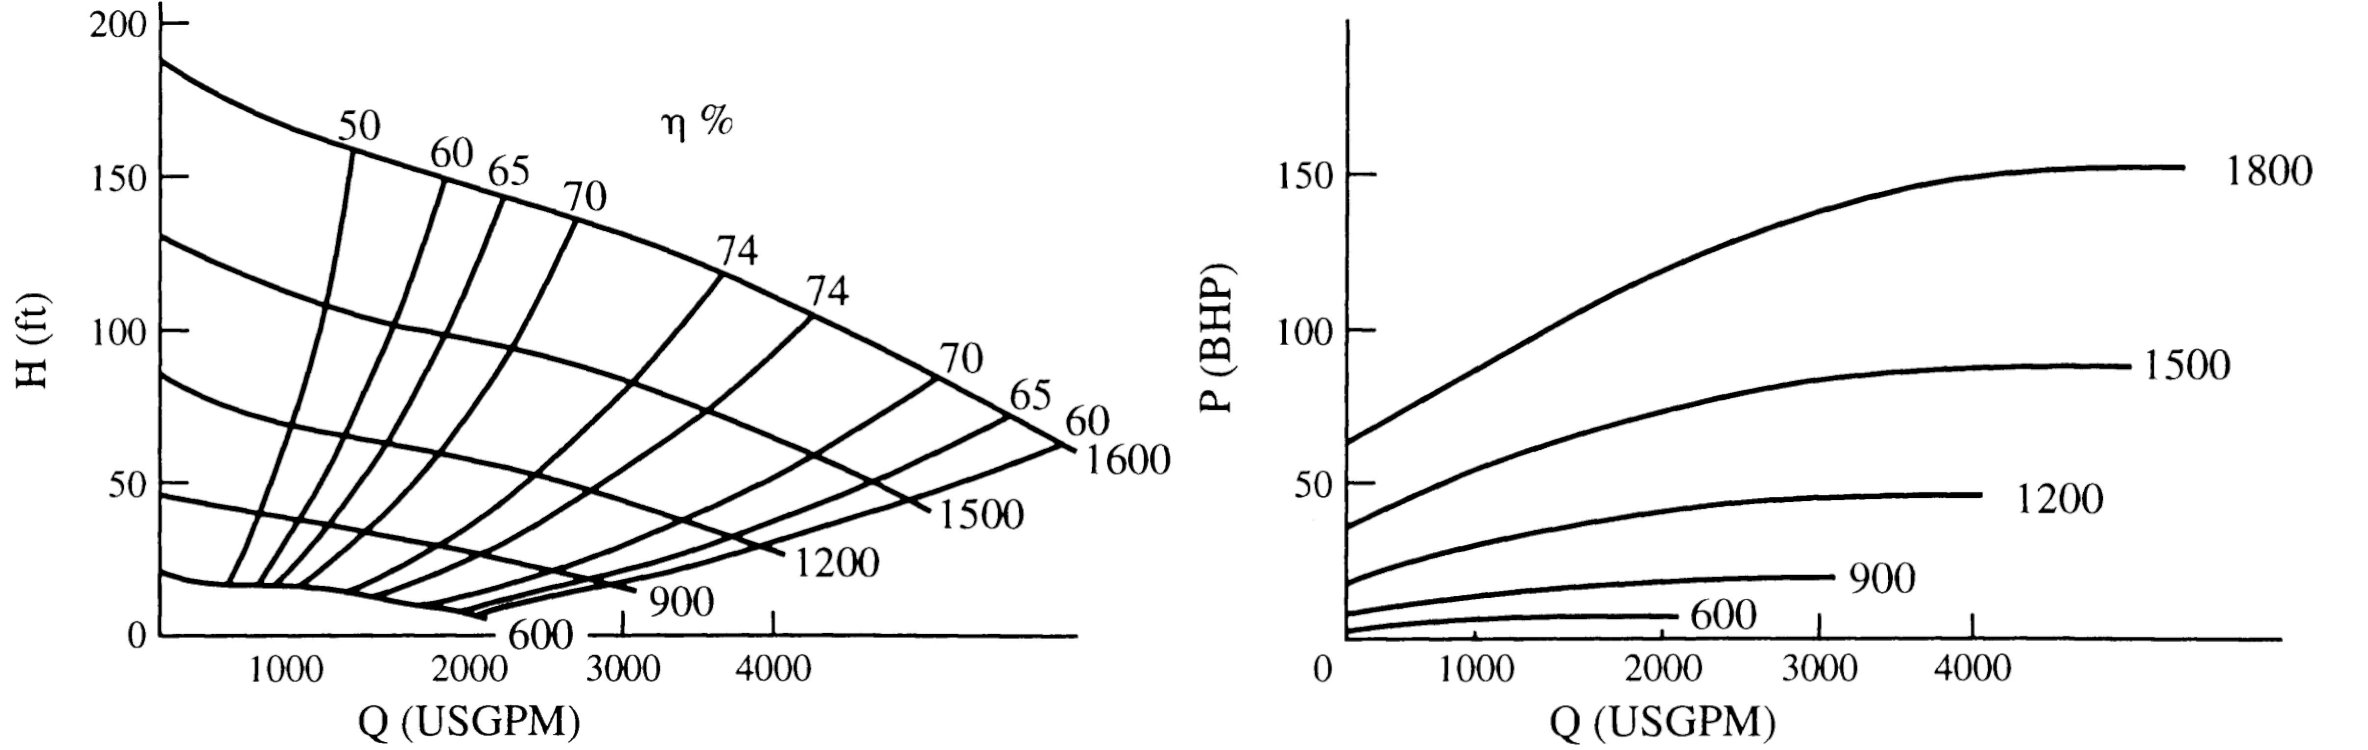
\includegraphics[width=0.8\textwidth]{char_map_pump.png}
    \caption{Characteristic maps of a pump \cite{Hillewaert2019}.}
    \label{fig:C4_MapPump}
\end{figure}

However, not all the operating points constituting the performance map have to be computed through an experimental campaign. Indeed, using the similarity analysis described during the previous section, determining the operating points for one rotational speed is sufficient to deduce the rest of the characteristic map.

\begin{subequations}
    \begin{equation}
        \phi = \frac{Q}{N\cdot r_2^3}\label{eq:C4_phipump}
    \end{equation}
    \begin{equation}
        \psi = \frac{4\cdot g\cdot \Delta h_p}{N^2\cdot r_2^2}\label{eq:C4_psipump}
    \end{equation}
\end{subequations}

For the pump, the head and flow non-dimensional coefficients \(\phi\) and \(\psi\) are defined based on the outlet condition \textbf{2} of the pump. Those coefficients are respectively defined by the relations (\ref{eq:C4_phipump}) and (\ref{eq:C4_psipump}), \(r_2\) being the outlet radius of the pump. 

From the definitions of these two non-dimensional quantities, the height variation \(\Delta h_p\) and the volumetric flow rate $Q$ can be obtained for any rotational speed. 

Considering that the operating point (\(Q_1, \Delta h_{p,1},N_1\)) is known, the similar operating point\linebreak (\(Q_2, \Delta h_{p,2},N_2\)) for any rotational speed \(N_2\) can be obtained using the relations (\ref{eq:C4_Qsim}) and (\ref{eq:C4_DHsim}).

\begin{subequations}
    \setstretch{1}
    \begin{equation}
        Q_2 = Q_1\cdot\frac{N_2}{N_1} \label{eq:C4_Qsim}
    \end{equation}
    \begin{equation}
        \Delta h_2 = \Delta h_1\cdot\left(\frac{N_2}{N_1}\right)^2 \label{eq:C4_DHsim}
    \end{equation}\label{eq:C4_sim}
\end{subequations}

These relations stand since for any similar point of operation, the non-dimensional quantities remain constant. Consequently, the pump isentropic efficiency remains constant as well.

Similar reasoning can be performed for the hydraulic turbines. For hydraulic turbines, the head and flow coefficients are defined based on the inlet condition \textbf{1} of the turbine.

% \subsubsection{Types of pumps and hydraulic turbines}
% \quad\ Now that the exterior characteristics of the turbomachines  have been defined, it is interesting to have at least a brief idea about how the pump is constructed. Without entering into detailed\footnote{see the section 4.3 and 4.4 of the course \cite{Hillewaert2019}}, there are two types of pumps.

% The first type to be considered is the centrifugal pumps designed to provide a high heat for a low flow rate. Those pumps are characterized by an axial inflow and a radial outflow. The Figure \ref{fig:C4_centri_pump} shows a schematic of a centrifugal pumps.
% \begin{figure}[h]
%     \centering
%     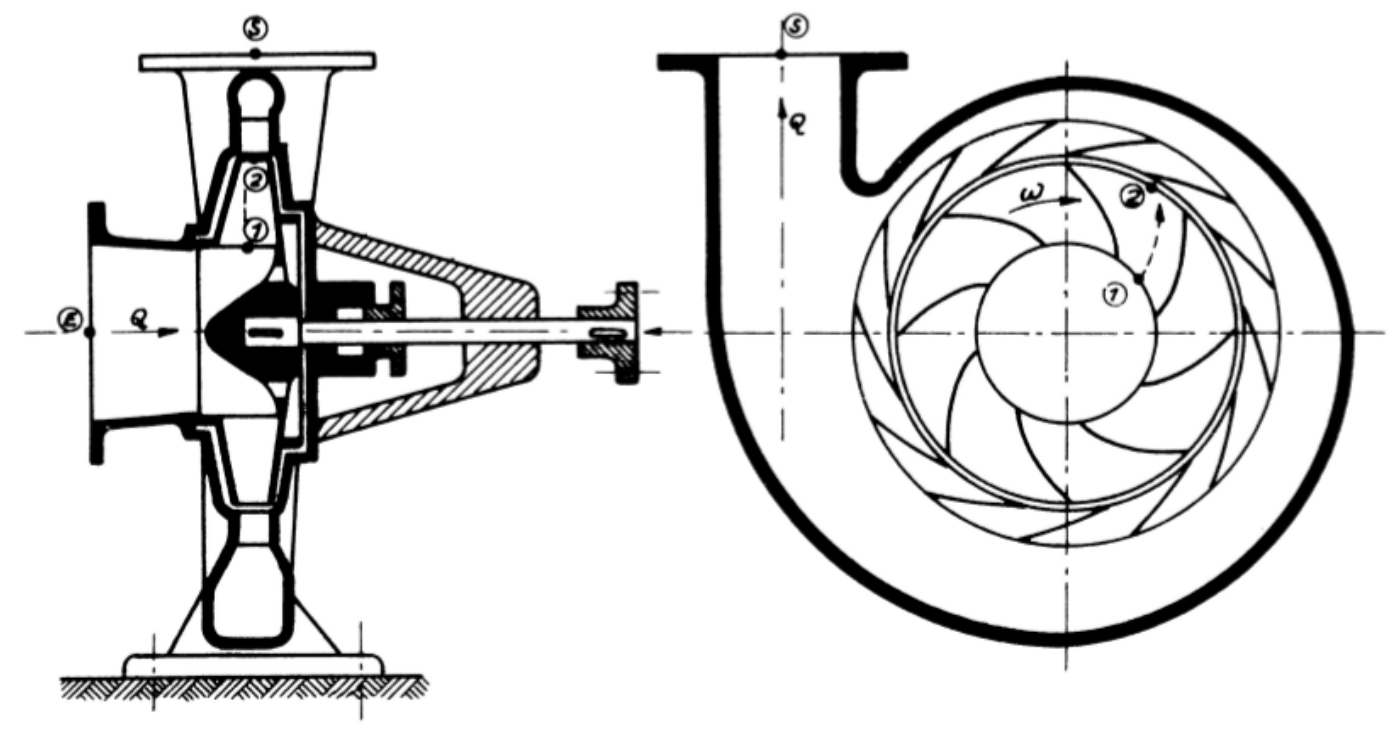
\includegraphics[width=0.4\textwidth]{centri_pump.png}
%     \caption{Centrifugal pump \cite{Hillewaert2019}.}
%     \label{fig:C4_centri_pump}
% \end{figure}

% Basically, the centrifugal pump can be decomposed into two parts (for the simplest machine). The first  part is the rotating impeller that will convert and transfer the mechanical energy to the fluid. Behind the impeller will be placed the volute (right picture of Figure \ref{fig:C4_centri_pump}) that collects the flow to bring it to the outlet of the pump.\newpage

% The second type of pump are the axial pumps which are, in opposition with the centrifugal pumps, designed to deliver low head for high flow rates. Such pumps are illustrated on Figure \ref{fig:C4_axial_pump}.
% \begin{figure}[h!]
%     \centering
%     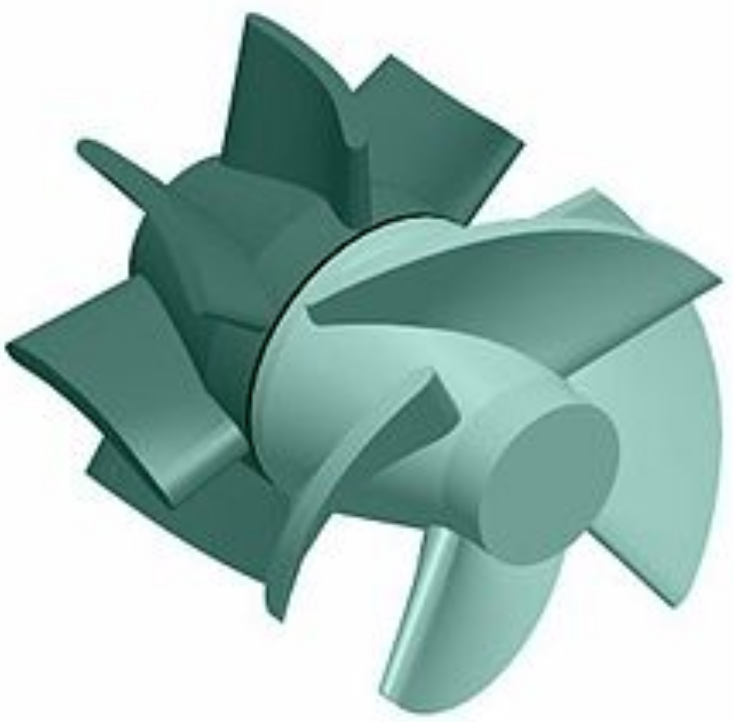
\includegraphics[width=0.25\textwidth]{axial_pump.png}
%     \caption{Axial pump \cite{Hillewaert2019}.}
%     \label{fig:C4_axial_pump}
% \end{figure}

% The main two parts of an axial pump are the rotor (the rotating part) that will increase the height of the fluid followed by a diffusor which “recuperates the kinetic energy at the exit of the rotor”\cite{Hillewaert2019}.
\subsection{Compressible flow}
\quad\ The previous subsection introduced the pump which is a turbomachine design to increase the energy of the incompressible fluid passing through it. However, this type of machine cannot deals with compressible flow for which the density can vary over the distance. For instance, the air is a compressible fluid.

The behavior of the compressible flow is more complex to describe compared to incompressible flow. Indeed, “compressible flow is characterized by the propagation of acoustic waves” \cite{Hillewaert2019}.   This part of the section about turbomachines will only focused on the very main principles required for the good understanding of this work.


\subsubsection{Velocity triangle}
\quad\ With the relation (\ref{eq:C4_Euler}), the notion of absolute and relative velocity of the flow has been introduced. A graphic representation of these three vector can be done using the \textbf{velocity triangle}. This triangle is drawn on Figure \ref{fig:C4_vtriang}.

\subsubsection{Mach number}
The Mach number \(M\) is defined as being the ratio between the velocity \(v\) and the sound speed \(a\).
\begin{equation}
    M = \frac{v}{a} \label{eq:C4_Mach}
\end{equation}
The Mach number \(M\) is a dimensionless variable that gives an image of the compressible effects of the flow. Thus, one criteria for the determination of similar operational points is to keep constant the Mach number.

Using the Mach number allows to obtain formulas to compute the total quantities base the static ones. By considering first the total temperature, it can be found
\begin{equation}
    T^0 = T + \frac{v^2}{2\cdot c_p} = T\cdot\left(1 + \frac{v^2}{2\cdot c_p\cdot T}\right)\label{eq:C4_TT0_1}
\end{equation}
For an isentropic process, it can be demonstrate that the speed of sound \(a=k\cdot r\cdot T\). Thus, the equation (\ref{eq:C4_TT0_1}) becomes
\begin{equation}
    T^0 = T\cdot\left(1 + \frac{k-1}{2}\cdot M^2\right) = T\cdot f(M) \label{eq:C4_TT0}
\end{equation}
Using the equations (\ref{eq:C3_isrelPT}), (\ref{eq:C3_isrelrhoT}) and the definition of the function \(f(M)\), the relations linking the static to the total pressure, density and speed of sound can be obtained as well.

\begin{subequations}
    \setstretch{1}
    \begin{equation}
        p^0 = p\cdot f(M)^\frac{k}{k-1}\label{eq:C4_PP0}
    \end{equation}
    \begin{equation}
        \rho^0 = \rho\cdot f(M)^\frac{1}{k-1}\label{eq:C4_rhorho0}
    \end{equation}
    \begin{equation}
        a^0 = a\sqrt{f(M)} \label{eq:C4_aa0}
    \end{equation}
\end{subequations}

\subsubsection{Characteristic maps}
\quad\ As for the turbomachines exchanging energy with incompressible flow, those dealing with compressible flow can also be fully characterized knowing a pair of independent operating parameters. The most usual parameters are

\begin{itemize}
    \setstretch{1}
    \item \(\dot{m}_c\) (kg/s or lbs/min): It is the corrected mass flow rate.

    \item \(N\) (rpm): It is the rotational speed of the turbomachine shaft.

    \item \(\Pi_{tt}\) (-): It is the total to total pressure ratio between the inlet and the outlet of the turbomachines. If the turbomachines is compressing the flow, the ratio is reverse to keep it greater than one.

    \item \(\eta_{tt}\) (-): It is the total to total isentropic efficiency of the machine.
\end{itemize}
The corrected mass flow rate is defined as being the flow that would observed at the prescribed \textbf{static} reference conditions ($T_{ref},P_{ref}$). Using the similarity, the relation (\ref{eq:C4_mc}) allows to derived the corrected mass flow rate.

\begin{equation}
    \dot{m}_c = \dot{m}\cdot \sqrt{\frac{T}{T_{ref}}}\cdot\left(\frac{p_{ref}}{p}\right)\label{eq:C4_mc}
\end{equation}

Alternatively, the reduced mass flow rate \(\dot{m}_r\)can also be used to assess the performance of the turbomachines. This non-dimensional quantity is as follows:
\begin{equation}
    \dot{m}_r = \dot{m}\cdot \frac{\sqrt{T}}{p}
\end{equation}

Let's supposed now that the rotational speed and the corrected mass flow are known. Then, the two other quantities ($\Pi$) and ($\eta$) can be calculated by evaluating the relationships (\ref{eq:C4_Pimap}) and (\ref{eq:C4_etamap}).

\begin{subequations}
    \setstretch{1}
    \begin{equation}
        \Pi_{tt} = \Pi_{tt}(N, \dot{m}_c)\label{eq:C4_Pimap}
    \end{equation}
    \begin{equation}
        \eta_{tt} = \eta_{tt}(N, \dot{m}_c)\label{eq:C4_etamap}
    \end{equation}
\end{subequations}
These relations can be established by the means of experimental measurements.
\subsection{Gas compressor}
\quad\ The previous lines shows some properties of compressible flows that add complexity to the analysis. Now, it is interesting to describe two types of turbomachines inducing a modification of the state of the flow.

The first machines to be describe are the compressor. As for the pumps, the compressor can be axial or centrifugal.  The axial compressor are mainly composed of a rotating part (the rotor), followed by a non moving part (the stator) converting the the kinetic energy at exit of the rotor into pressure. A schematic of an axial compressor stage is given on Figure \ref{fig:C4_compstage}.

\begin{figure}[h]
    \centering
    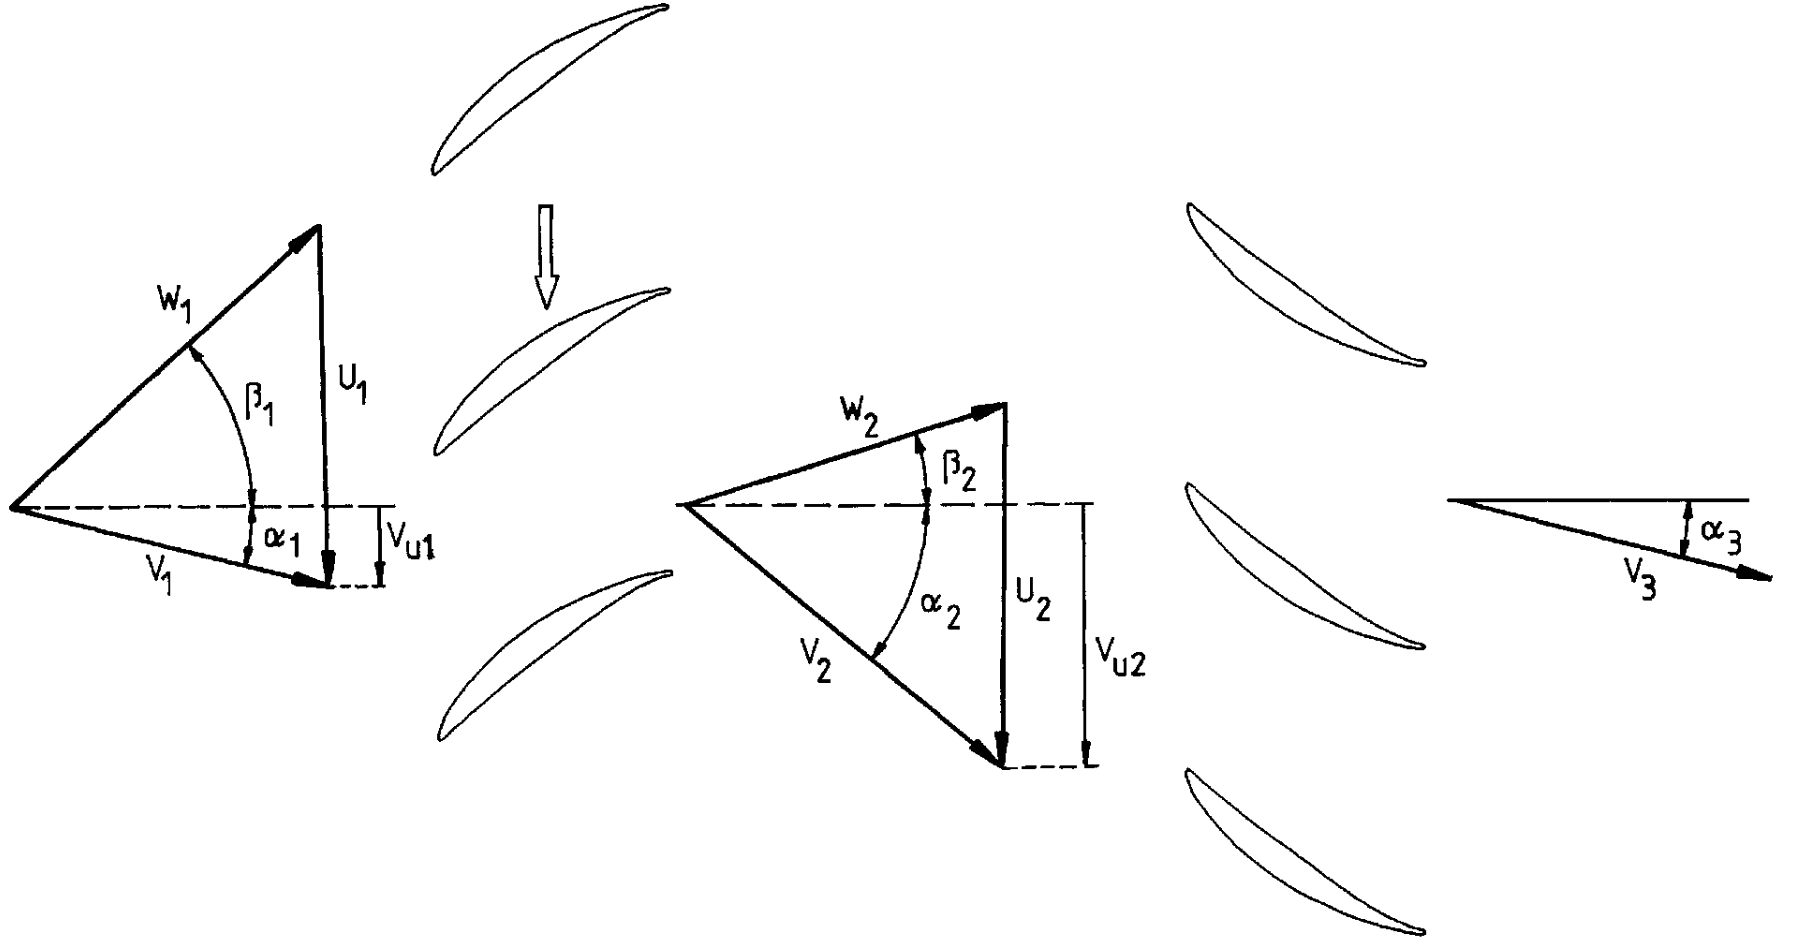
\includegraphics[width=0.5\textwidth]{Comp_stage.png}
    \caption{Axial compressor stage \cite{Hillewaert2019}.}
    \label{fig:C4_compstage}
\end{figure}

The entities between each velocity triangles are the blades of the rotor (emphasized by an arrow) or of the stator. It can be observed that the rotor blades increase the value of the flow velocity \(v\). As explained earlier this augmentation of kinetic energy is then recovered by the stator blades.

\subsubsection{Mollier diagram}
\quad\ The transformation induced by the compressor can be represented into a hs diagram also named the Mollier diagram. The Mollier diagram for one compressor stage has been drawn on Figure \ref{fig:C4_Molliercomp}.

\begin{figure}[h]
    \centering
    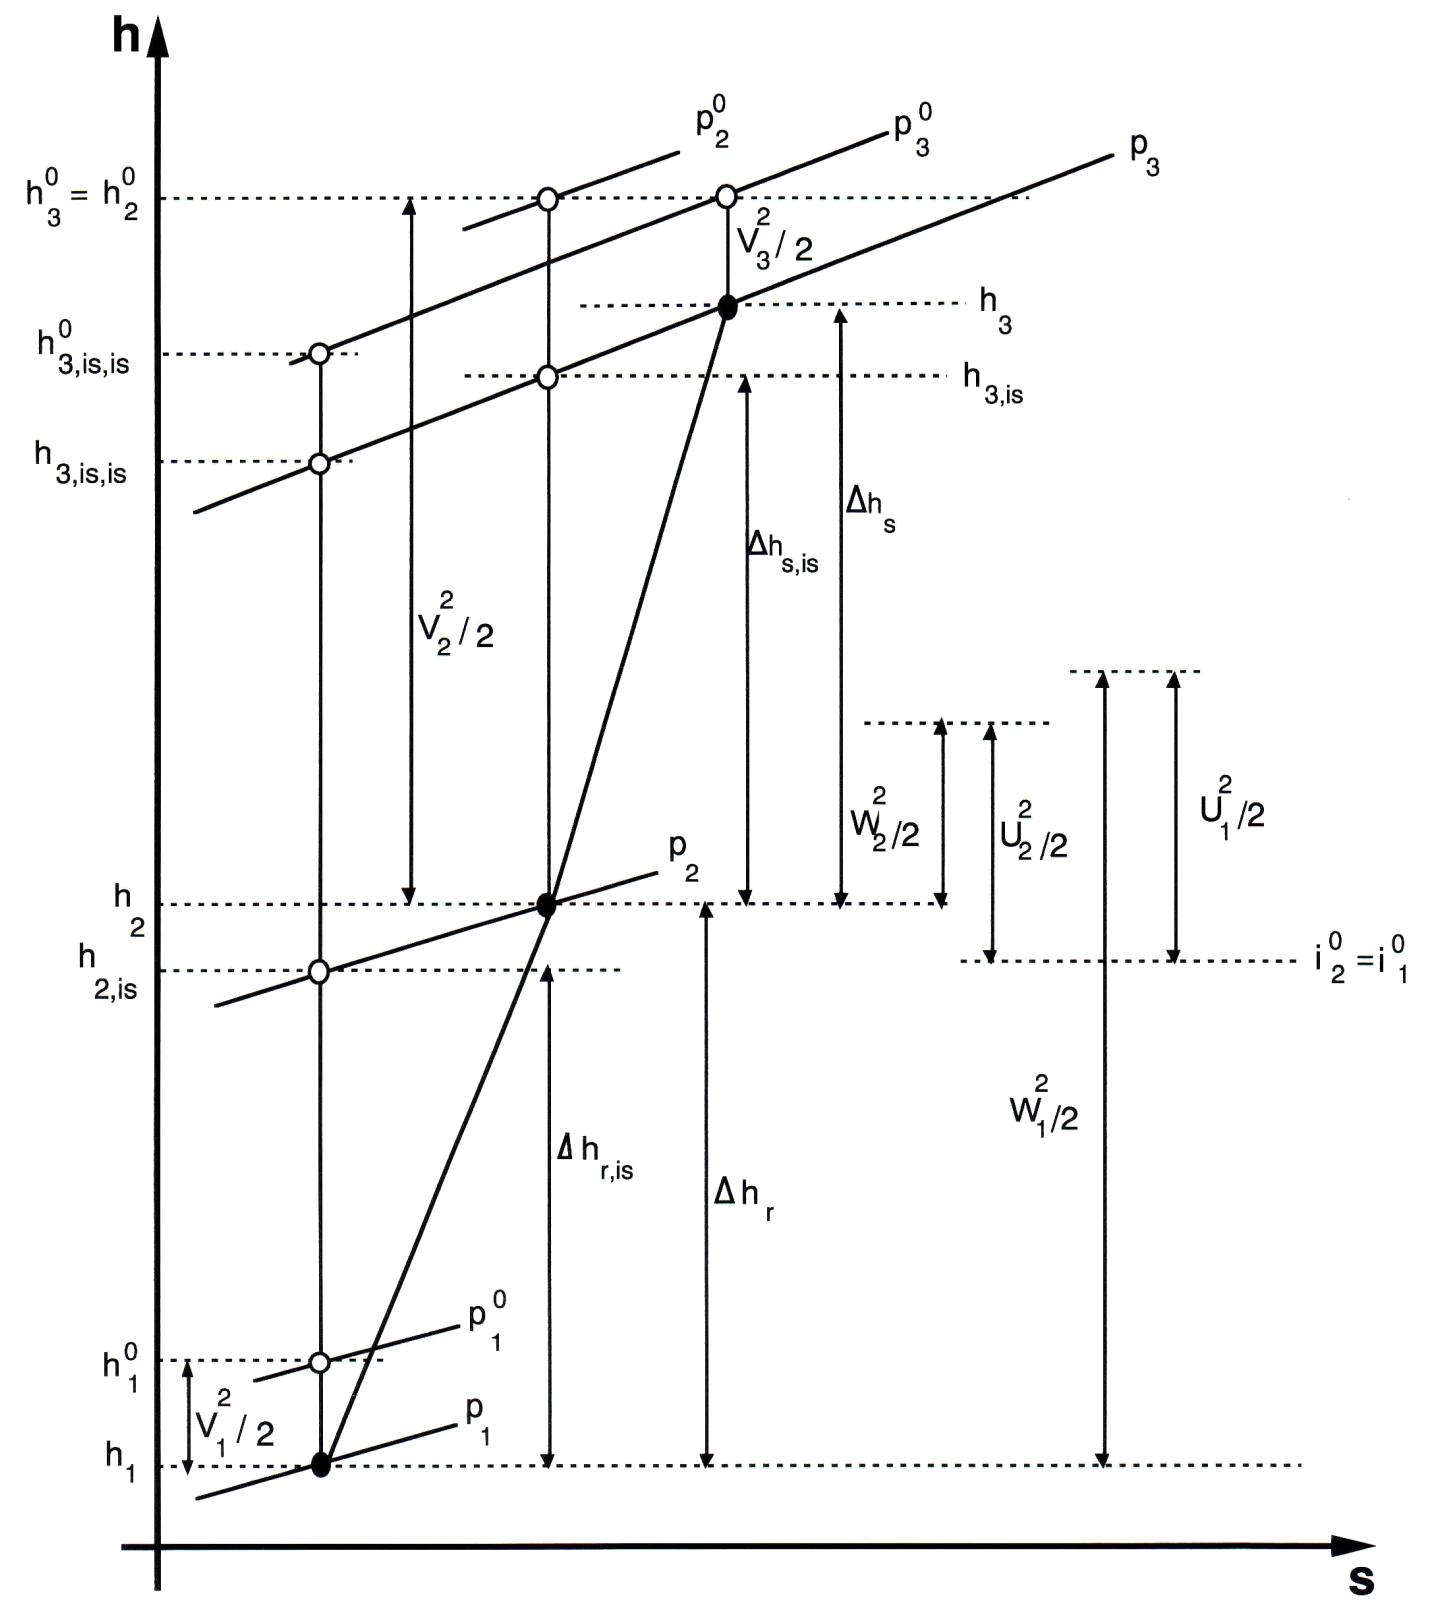
\includegraphics[width=0.5\textwidth]{Comp_mollier.png}
    \caption{Mollier diagram of a compressor stage \cite{Hillewaert2019}}
    \label{fig:C4_Molliercomp}
\end{figure}

The diagram, for which the velocity triangles are given on Figure \ref{fig:C4_compstage}, has to be read as follows.
\begin{itemize}
    \setstretch{1}
    \item State \textbf{1}: Starting from the static enthalpy and pressure \(h_1\) and \(p_1\), the relations (\ref{eq:C4_i0}), (\ref{eq:C4_h0}) and (\ref{eq:C4_PP0}) are used to calculate the total enthalpy, rothalpy and pressure.
    \item State \textbf{2}: The transformation \textbf{1}-\textbf{2} takes place within the rotor of the compressor stage. Thus, the total rothalpy is conserved over the transformation ($i_2^0=i_1^0$).

    The knowledge of the total rothalpy allows to determine the other quantities. The static enthalpy (and by extension the total enthalpy) can be deduced using the relation (\ref{eq:C4_i0}). Concerning the pressure, there is an increase of the static and total pressure of the fluid “due to the diffusion in the rotor passage” \cite{Hillewaert2019} ($p_2^{(0)} > p_1^{(0)}$).

    \item State \textbf{3}: The transformation \textbf{2}-\textbf{3} takes place within the stator of the compressor stage. Thus, the total enthalpy is conserved over the transformation ($h_3^0 = h_2^0$).

    Then, the static enthalpy can be computed using the relation (\ref{eq:C4_h0}). The conversion of the kinetic energy into pressure leads to an increase of the static and total pressure ($p_3^{(0)} > p_2^{(0)}$).
\end{itemize}
As a reminder, the enthalpy at the end of the process is higher than the one considering an isentropic transformation.
\subsubsection{Performance maps}
\quad\ As for any turbomachines, the compressor can be characterized by its performance map. The map is composed of the performance plot often completed with the efficiency hill. The performance plot provides the total to total (TT) pressure ratio \(\Pi_{tt,c}\) as a function of the rotational speed \(N\) and the corrected flow rate \(\dot{m}_c\).

A illustration of a compressor performance map is given on Figure \ref{fig:C4_compmap}.
\begin{figure}[h]
    \centering
    \includegraphics[width=0.6\textwidth]{Comp_Map.png}
    \caption{Illustration of a compressor performance map \cite{Ghorbanian2009}.}
    \label{fig:C4_compmap}
\end{figure}

On the map, the solid and the dash curves represent respectively the iso-rotational speed and the iso-efficiency.

To remarkable lines are emphasized on the plot. For each rotational speed \(N_c\), these lines provides minimal and maximal bound for the compressor pressure ratio \(\Pi_{tt,c}\).

The lower limit is given by the choke line. “When the flow reaches the velocity at some cross-section” \cite{Ghorbanian2009}, an increase of the gas mass flow rate is not possible. Thus, the slope of the associated iso-rotational speed becomes equal to the infinity at this point. 

This limit is such that the mass flow rate of stall increases with the rotational speed. Indeed, it can be demonstrated that the maximal flow rate depends on the stagnation conditions of the flow. Thus, at the inlet of the compressor, the total conditions increases with the rotational speed. 

The upper bound is given by the “aerodynamic stability limit line'' or surge line. At this minimal flow rate, the flow start to stall in the machine. Going beyond this limit would lead to a backward flow in the compressor, causing irreversible damages to the compressor. Thus when operating the machine, a certain margin is taken with respect to the surge line.

At low rotational speeds, the flow can be supposed incompressible. Using this approximation, it is possible to use the rules of similarity described in the section about pumps to extrapolate the map to the lower rotational speed.

\subsection{Gas turbine}
\quad\ From now, only compressors have been introduced. However, in a gas cycle, the compressor are combined with a turbine that will expand the gas. Only for some exception, the turbine is always placed after the combustion chamber. This choice allows to provide to the turbine a flow with very high enthalpy.

Typically, an axial gas turbine is composed of a stator followed by a rotor. The stator is design to create a deflection of the flow in the sens of rotation of the rotor. This will accelerate the flow before entering the rotor.

The schematic of an axial turbine stage is drawn on Figure \ref{fig:C4_turbstage}.
\begin{figure}[h]
    \centering
    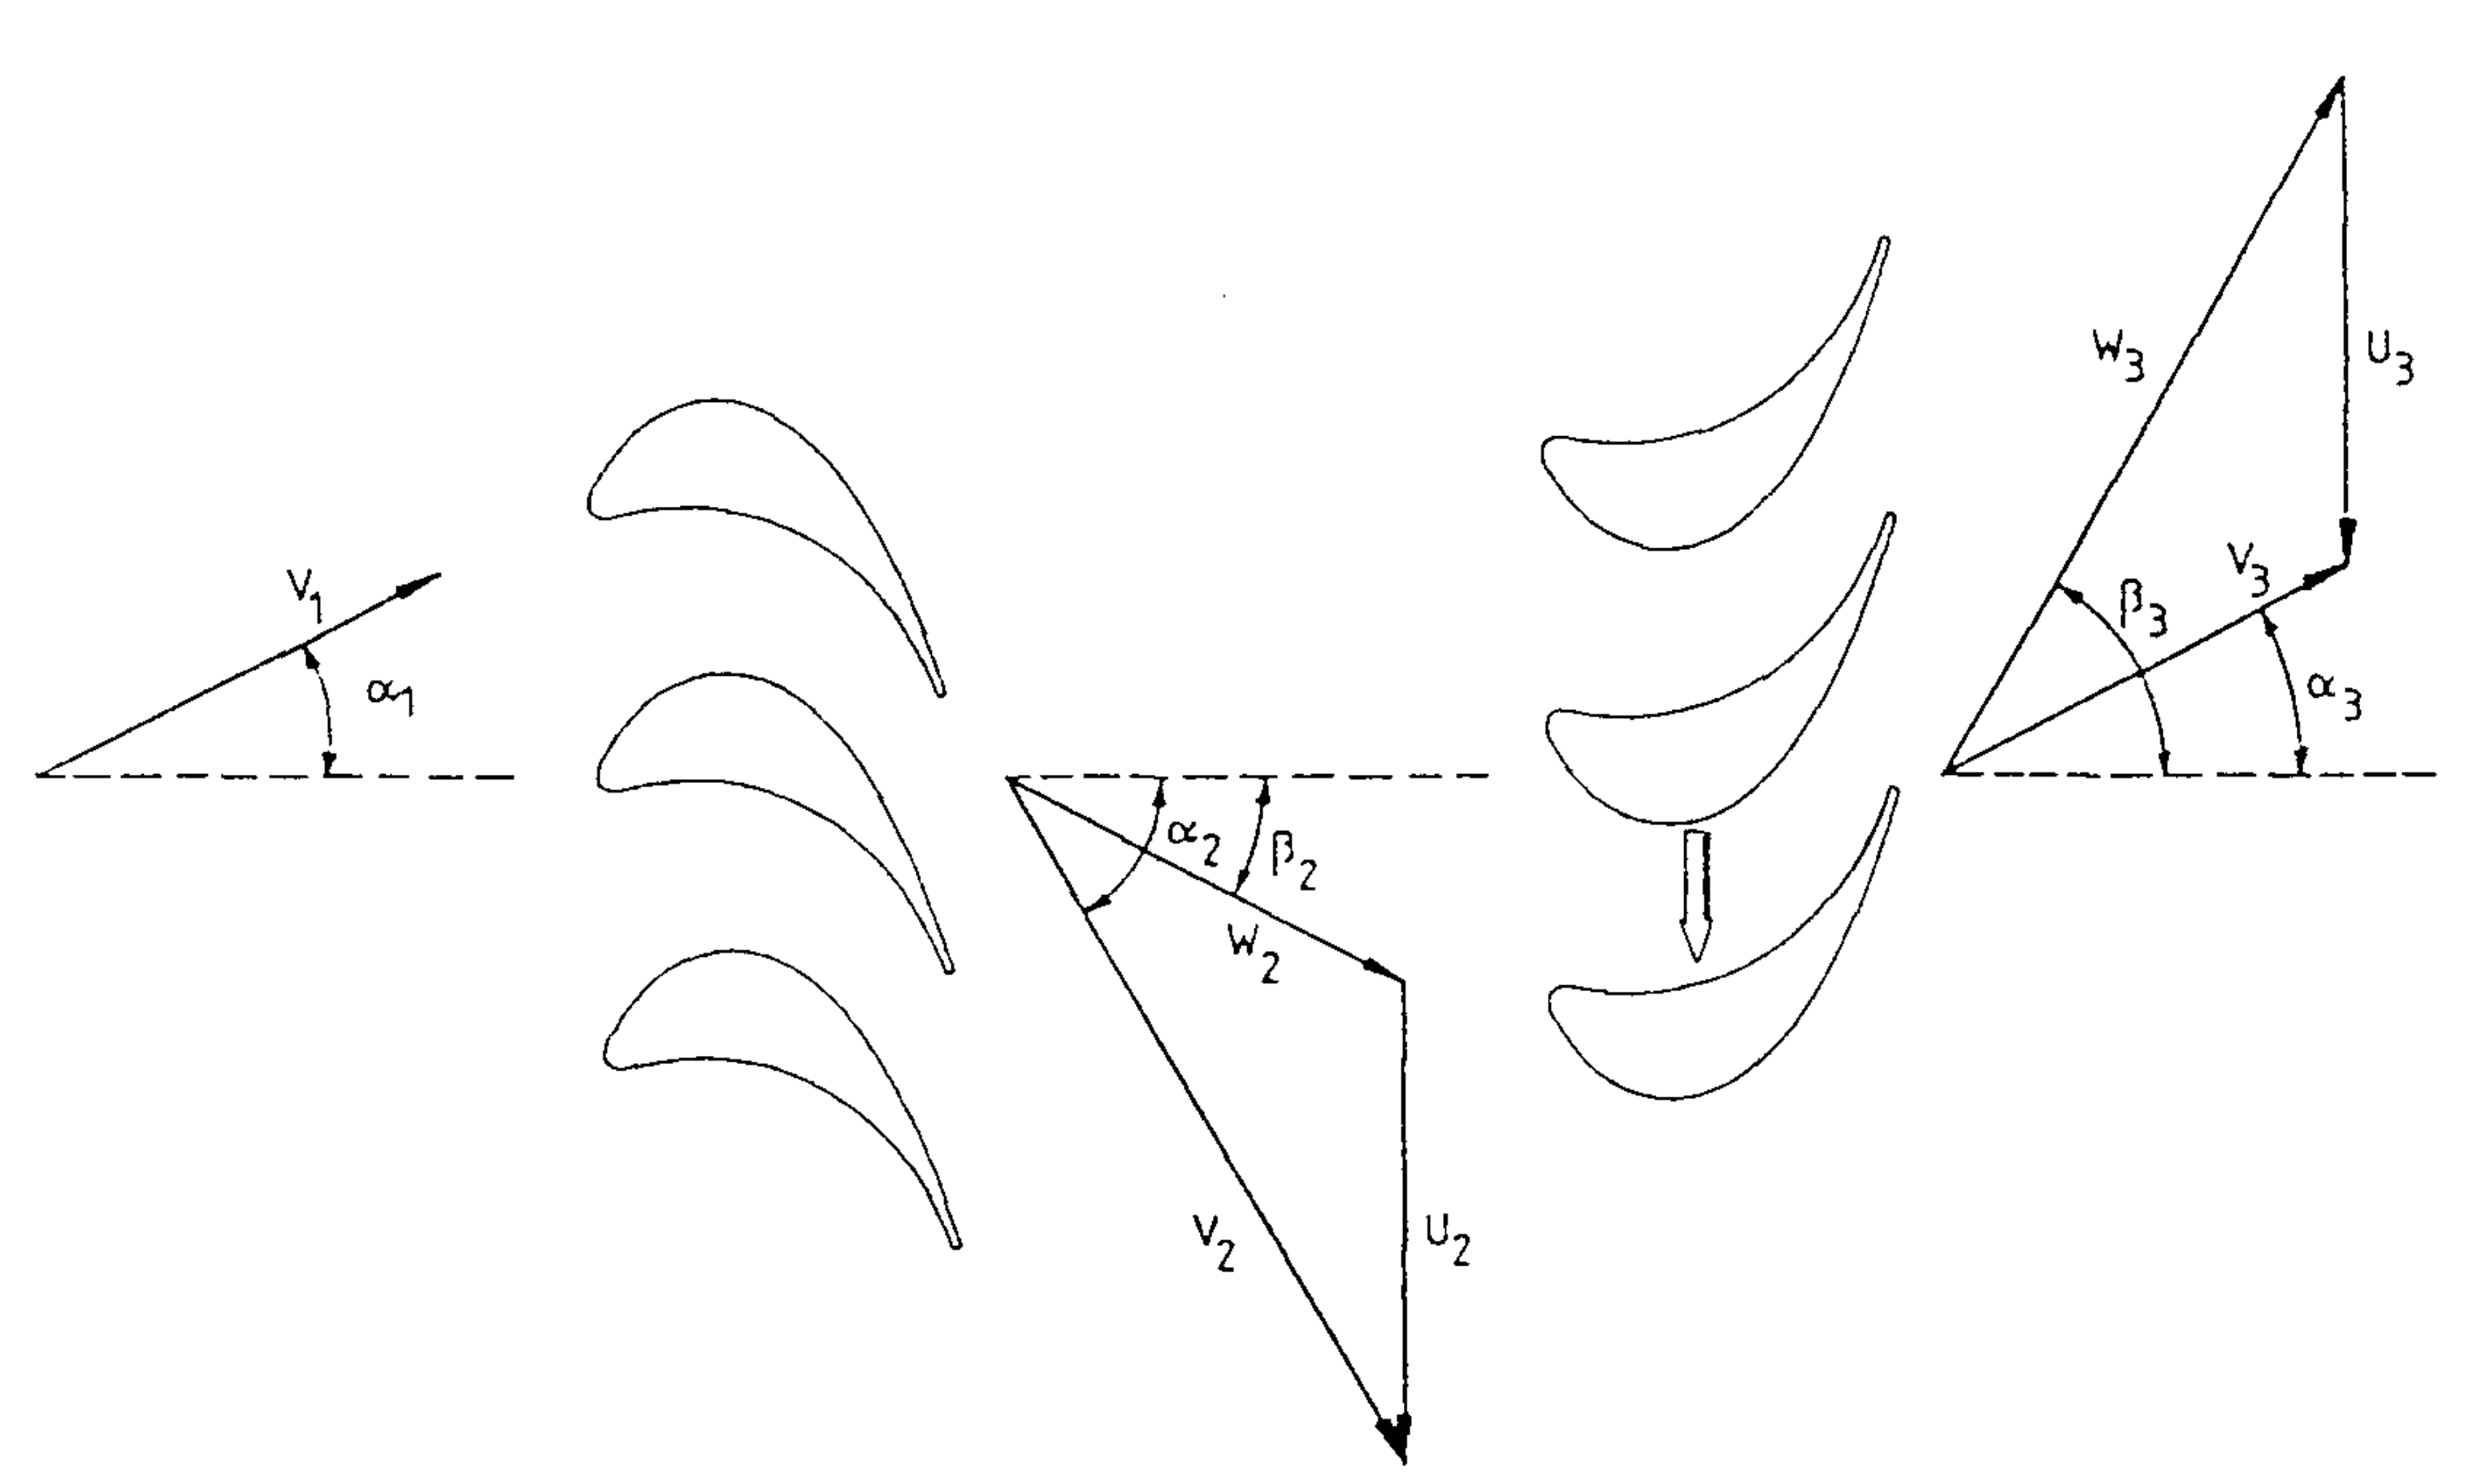
\includegraphics[width=0.5\textwidth]{Turb_stage.png}
    \caption{Axial turbine stage \cite{Hillewaert2019}.}
    \label{fig:C4_turbstage}
\end{figure}
\subsubsection{Mollier diagram}
As for the compressor, the real expansion induced by the turbine can be represented into a Mollier diagram. The diagram is depicted on Figure \ref{fig:C4_Mollierturb}. The methodology to read the diagram is the same as before.


\begin{itemize}
    \setstretch{1}
    \item State \textbf{1}: Starting from the static enthalpy and pressure, the total quantities can be deduced.
    \item State \textbf{2}: The transformation \textbf{1}-\textbf{2} takes place within the stator of the turbine stage. Therefore, the total enthalpy is conserved over the transformation ($h_2^0=h_1^0$).

    Knowing the total enthalpy of the state \textbf{2} allows to compute the static enthalpy and by extension the total rothalpy. Plus, since the flow is accelerated by the stator blades, the static and total pressure falls from state \textbf{1} to state \textbf{2} (\(p_2^{(0)}<p_1^{(0)}\)).
\end{itemize}

\begin{figure}[h]
    \centering
    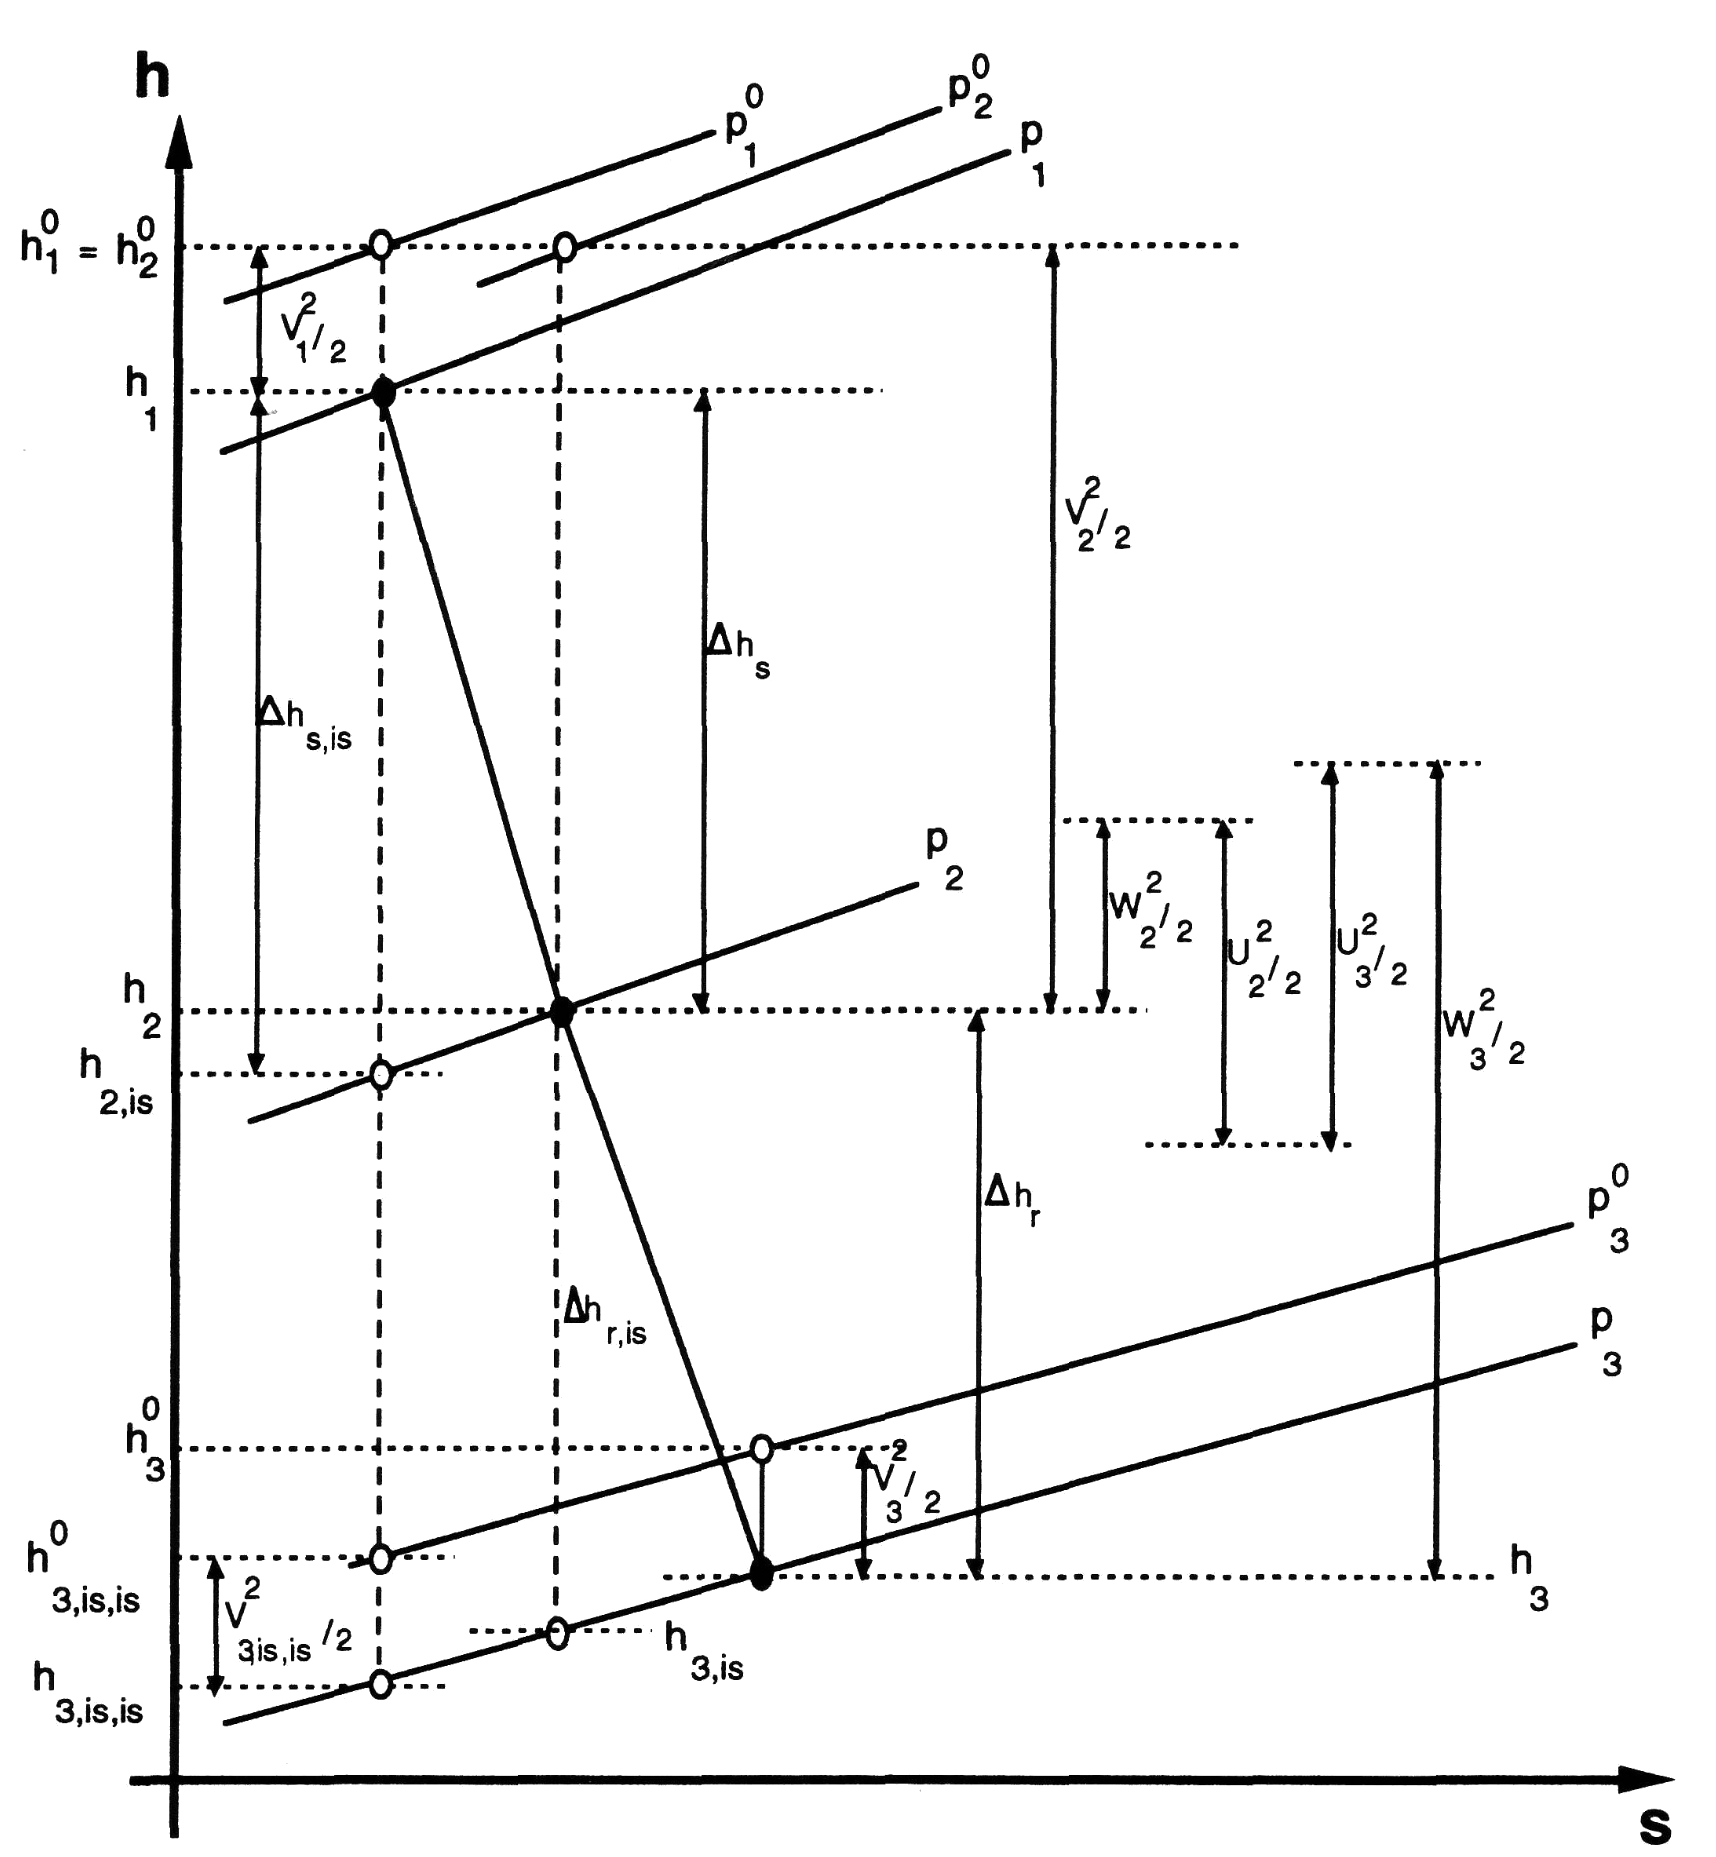
\includegraphics[width=0.5\textwidth]{Turb_mollier.png}
    \caption{Mollier diagram of a turbine stage \cite{Hillewaert2019}.}
    \label{fig:C4_Mollierturb}
\end{figure}

\begin{itemize}
    \item State \textbf{3}: The transformation \textbf{2}-\textbf{3} takes place within the rotor of the turbine stage. Therefore, the total rothalpy is conserved over the transformation (\(i_3^0=i_2^0\)).

    Then, the relation (\ref{eq:C4_i0}) allows to retrieve the static enthalpy of state \textbf{3}. As shown on the schematic \ref{fig:C4_turbstage} of the turbine stage, the relative speed of the flow is augmented when going through the rotor passage. This generates a second drop of the static and total enthalpy and pressure (\(p_3^{(0)}<p_2^{(0)}\)).

    However, there exists special stage for which “the relative velocity of the flow to the blade row” of the rotor\cite{Hillewaert2019} remains unchanged, but the flow is inverted. Neglecting the very small variation of the rotor velocity, the static enthalpy and pressure remains unchanged when passing through the rotor.
\end{itemize}


\subsubsection{Degree of reaction}
\quad\ The last written paragraph mentioned that some turbines are designed to put all the pressure drop over the stator to limit the axial force generated in the rotor.

In general, i is possible to classify the turbomachines by creating two categories based on the degree of reaction \(R\). The degree of reaction is defined as being the ratio between the static enthalpy drop (resp. raise) over the rotor and the static enthalpy drop (resp. raise) over the turbomachine stage.
\begin{equation}
    R = \frac{h_2 - h_3}{h_1 - h_3}\label{eq:C4_R}
\end{equation}
From this definition, the two categories can be defined as follows:

\begin{itemize}
    \setstretch{1}
    \item The impulse or action turbomachines: The degree of reaction \(R\simeq 0\). Thus, since the rotor doesn't see any pressure difference, the axial thrust on the shaft is minimized. 
    \item The reaction turbomacines: The degree of reaction \(R\) is often between 0.5 and 0.7. This means that the pressure drop is distributed between the stator and the rotor.
\end{itemize}

\subsubsection{Performance maps}
\quad\ The turbines can be also be characterized by a performance map determined from experimental results. The map is often composed of two performance plots as shown on Figure \ref{fig:C4_turbmap}.

\begin{figure}[h]
    \centering
    \includegraphics[width=\textwidth]{Turb_Map.png}
    \caption{Illustration of a turbine performance map \cite{Dixon2013}.}
    \label{fig:C4_turbmap}
\end{figure}

The two plots on the Figure \ref{fig:C4_turbmap} illustrates for each iso-rotational speed \(N_t\) the relationships \(\Pi_t(\dot{m}_c,N_t)\) and \(\eta_t(\dot{m}_c,N_t)\). 

As it can be noticed on the right diagram, all the curves are all stacked on each others when a certain pressure ratio is reached. Compared to the compressor, the choking phenomenon occurs for the same mass flow rate, regardless the rotational speed considered. 

For a turbine, the expansion is mainly performed within its statoric parts. This massive drop of the total pressure comes with a big increase of the kinetic energy of the flow. 

Therefore, it is within this part of the turbine stage that the choking phenomenon will likely occurs. Since the stator is not rotating, the maximal mass flow rate is not really impacted by the rotating speed of the rotor. This is the reason why all the iso-rotational speed curves have the same asymptotic value for the mass flow rate.


To summarize what have been seen in this section about turbomachines, the most important notions for the good understanding of the future development have been given. Particularly, the concept of performance maps has been introduced, and a method of extrapolation using the similarity have been provided.

Also, the descriptions of the compression and the expansion have been explained using the hs Mollier diagrams. Those diagrams, along with the schematic of the compressor and turbine stages, allow describing with a decent accuracy the two previously mentioned transformation.
\newpage
\section{Combustion chamber}
%%%%%%%%%%%%%%%%%%%%%%%%%%%%%%%%%%%
%%%%%                         %%%%%
%%%%% <<Combustion chamber>>  %%%%%
%%%%%                         %%%%%
%%%%%%%%%%%%%%%%%%%%%%%%%%%%%%%%%%%
\quad\ The previous section introduced the turbomachines and described those using schematic and hs diagram. The notion of compressible has been defined, and some important concepts have been emphasized.

In this section, the description of the combustion principle will be considered. Since the study of the fluid mechanic inside the combustion chamber is out of the scope of this work, only combustion equations without dynamic and non-steady effects will be considered.

\subsection{Basis about Chemistry}
\quad\ As it has been mentioned, some combustion reactions will be introduced in this section. Thus, the basic knowledge about chemistry has to be provided.

\subsubsection{Conservation of mass}
During a chemical reaction, the law of conservation of mass (also called the Lavoisier law) has to be satisfy. This implies that the mass of all the reagents combined has to be equal to the mass of the products. An example of chemical reaction is given in (\ref{eq:C4_chem}).

\begin{equation}
    \setstretch{1}
    \underset{\mathrm{16g}}{\ce{1CH4}} \ce{+} \underset{\mathrm{64g}}{\ce{2O2}} \ce{->} \underset{\mathrm{44g}}{\ce{1CO2}} \ce{+} \underset{\mathrm{36g}}{\ce{2H2O}} \ce{+}\text{Heat}\label{eq:C4_chem}
\end{equation}

It will be seen later that this reaction corresponds to the combustion of \textbf{1} mole of methane (\ce{CH4}) using \textbf{2} mole of oxygen (\ce{O2}). The products of the reaction are \textbf{1} mole of \ce{CO2}, \textbf{2} moles of \ce{H2O} and a certain amount of heat transfer to the surrounding. This heat transfer is the wanted product of the combustion.

\subsubsection{Conservation of the atomic species}
The second law of conservation states that, during the transformation of the reagent X into the product Y, all the atomic elements from X have to be recovered in Y. For instance, for the equation (\ref{eq:C4_chem}), there is one mole of carbon (\ce{C}) in the reagents. Thus, one mole of \ce{C} has to be present in the products of the reaction.
\newpage
\subsubsection{Proust's law}
The third law to be considered is the Proust law which states that for each chemical reactions, ''the ratio between the mass of each reagent is a constant''. Considering the above example (\ref{eq:C4_chem}), this implies that the ratio

\begin{equation}
    \setstretch{1}
    \frac{\text{mass of \ce{O2} consumed}}{\text{mass of \ce{CH4} consumed}} = 4
\end{equation}

Let's remark that the law is also valid considering the consumed quantities in mole. This would lead to the following relation

\begin{equation}
    \setstretch{1}
    \frac{\text{mole of \ce{O2} consumed}}{\text{mole of \ce{CH4} consumed}} = 2  \label{eq:C4_molratio}
\end{equation}

This ratio depends on the type of fuel used. For instance, if the fuel was propane (\ce{C4H8}), the ratio would be equal to 5.

\subsection{Combustion equation}
\quad\ The equation \ref{eq:C4_chem} was illustrating the combustion of the methane \ce{CH4}. The reaction, as written there, supposed that the provided amount of oxygen provided for the reaction is just enough to consume all the methane injected.

This situation, which is the reference, is characterized by an air factor \(\lambda = 1\) (or an excess of air \(e=\lambda-1=0\)). It is said that such combustion is at the stoichiometry.

\subsubsection{Air factor}
The air factor is then defined as being the ratio between

\begin{equation}
    \setstretch{1}
    \lambda = \frac{\frac{\text{mole of \ce{O2} consumed}}{\text{mole of fuel consumed}}}{\frac{\text{mole of \ce{O2} consumed at stoichiometry}}{\text{mole of fuel consumed at stoichiometry}}} \label{eq:C4_lbd}
\end{equation}

Let's note that every other combustive can replaced the oxygen in the relation. However, \ce{O2} is the most common one. Thus, the following development will not consider this possibility.
For the following, the notation \(w_{\ce{\text{<molecule>}}}\) will be used in replacement for ''mole of <molecule> consumed''.

For the case of the \ce{CH4} being the fuel, it has been shown in the previous section that the value of the denominator of relation (\ref{eq:C4_lbd}) is equal to 2. Therefore, for this particular combustion, the air factor relation is
\begin{equation}
    \setstretch{1}
    \lambda = \frac{w_{\ce{O2}}}{2\cdot w_{\ce{CH4}}}\label{eq:C4_lbdCH4}
\end{equation}

\subsubsection{Generalized combustion equation}
\quad\ As explained, the chemical reaction (\ref{eq:C4_chem}) represents the ideal case with an air factor of 1. Also, it is considered that the used combustive is pure \ce{O2}. In reality, the used reagent for the combustion is ambient air which is composed of 21\% of \ce{O2} and 79\% of \ce{N2} (nitrogen).

Thus, the generalized combustion equation (for the \ce{CH4}) is defined as in the reaction (\ref{eq:C4_chemgeng0}).

\begin{equation}
    \setstretch{1}
    \ce{CH4 +}2\lambda \left(\ce{O2}+\frac{79}{21}\ce{N2}\right) \ce{-> CO2 + 2(\lambda-1)O2 + 2H2O + 2\lambda\frac{79}{21}N2 + \text{Heat}}\label{eq:C4_chemgeng0}
\end{equation}

This equation, while being correct for any values of \(\lambda\) greater or equal than 1, has to be modified to take into account the event for which the excess of air \(e\) is lower than zero (with \(e=\lambda -1\)). For such values, the combustion equation then becomes as stated in (\ref{eq:C4_chemgeng1}).

\begin{equation}
    \setstretch{1}
    \ce{CH4 +}2\lambda \left(\ce{O2}+\frac{79}{21}\ce{N2}\right) \ce{-> aCO2 + bCO + 2H2O + 2\lambda\frac{79}{21}N2 + \text{Heat}}\label{eq:C4_chemgeng1}
\end{equation}

where coefficients ''a'' and ''b'' satisfies the system (\ref{eq:C4_sysab})

\begin{equation}
    \setstretch{1}
    \begin{cases}
        \text{a} + \text{b} = 1 \\
        2\text{a} + \text{b} = 4\lambda - 2
    \end{cases}\label{eq:C4_sysab}
\end{equation}

where both equations have been obtained based on the conservation of the atomic species. It can be calculated that there exists a lower bound for the air factor below which the combustion will be impossible. The condition is that the coefficient ''a'' cannot be smaller than zero. For this case, the minimal air factor \(\lambda_{min} =-\frac{3}{4}\).

To provide some definitions, the mixture oxygen-fuel is said poor when \(\lambda>0\), rich when \(\lambda<0\) and at the stoichiometry for an air factor \(\lambda=1\). Typically, for a gas turbine the mixture is very poor with a $\lambda$ often greater than 4-5.

\subsection{Fuel characteristic}
\quad\ From now, the amount of heat provided during the combustion has not been quantified. This quantification is really important because this amount of heat is linked to quality and the nature of the used fuel.

\subsubsection{Heating calorific value}
\quad\ First, let's define the heating calorific value \(HCV\) of a fuel (J/kg). By definition, it is ''the amount of thermal energy released during the total combustion of one physical unit of fuel” \cite{Leonard2018}.

\begin{equation}
    \setstretch{1}
    HCV = -\Delta H^o_{combustion} \label{eq:C4_HCV1}
\end{equation}

with \(-\Delta H^o_{combustion}\) being the heat released during the reaction.

The \(HCV\) is determined at a given reference temperature \(T_0\). Considering this reference temperature, the \(HCV\) can be evaluated by computing the enthalpy difference between the reagents and the products.

\begin{equation}
    \setstretch{1}
    HCV = \left.h_{reagent}\right|_{T=T_0} - \left.h_{product}\right|_{T=T_0}\label{eq:C4_HCV2}
\end{equation}

Distinction between the lower and higher heating calorific value (respectively $HCV_l$ and $HCV_h$) have to be made. Basically, when considering the combustion of a given fuel, the amount of energy released corresponds to the lower heating calorific value if the water remains gaseous within the exhaust gas. 

However, when the water contained in the exhaust gas have been condensed into liquid water, the energy released from the phenomenon is added to the lower HCV. For this case, the higher heating calorific value is then used instead of the lower one.  

The \(HCV\) value depends on the type of fuel that is used. For example, the lower heating calorific value of the \ce{CH4} is around 50 MJ/kg.

\subsubsection{Adiabatic flame temperature}
\quad\ The second notion that can be defined is the adiabatic flame temperature \(T_f\). If the combustion chamber is supposed to be adiabatic (no heat transfer to the outside), the heat generated will be fully retained within the exhaust gas of the combustor. Thus, the temperature reached by the gas is considered to maximal and is called the adiabatic flame temperature.

The evaluation of \(T_f\) is quite similar to the one of the \(HCV\). There, starting from the reference temperature, the \(T_f\) is calculate such that the enthalpy of the products is equal to the enthalpy of the reagents.

\begin{equation}
    \setstretch{1}
    \left.h_{reagent}\right|_{T=T_0} = \left.h_{product}\right|_{T=T_f}\label{eq:C4_T_f}
\end{equation}

\subsection{Fumes composition}
\quad\ Previously has been presented in the equations (\ref{eq:C4_chemgeng0}) and (\ref{eq:C4_chemgeng1}) the generalized chemical reaction for the combustion of the methane.
In a more general case, if the fuel is essentially composed of carbon \ce{C}, hydrogen \ce{H}, oxygen \ce{O} and nitrogen \ce{N}, the reactions (\ref{eq:C4_chemgeng0}) and (\ref{eq:C4_chemgeng1}) are then given in (\ref{eq:C4_chemgeng01}).

\begin{equation}
    \setstretch{1}
    \begin{cases}
        \ce{C_{\text{m}}H_{\text{n}}O_{\text{x}}N_{\text{y}} +}\kappa\lambda \left(\ce{O2}+\frac{79}{21}\ce{N2}\right) \ce{-> mCO2 +} \kappa(\lambda-1)\ce{O2 + \frac{n}{2}H2O +} (\kappa\lambda\frac{79}{21} + \frac{\text{y}}{2})\ce{N2} & \text{ for \(\lambda\geq 1\)} \\
        \ce{C_{\text{m}}H_{\text{n}}O_{\text{x}}N_{\text{y}} +}\kappa\lambda \left(\ce{O2}+\frac{79}{21}\ce{N2}\right) \ce{-> aCO2 + bCO + \frac{n}{2}H2O} + (\kappa\lambda\frac{79}{21} + \frac{\text{y}}{2})\ce{N2}                      & \text{ for \(\lambda< 1\)}
    \end{cases}\label{eq:C4_chemgeng01}
\end{equation}

where coefficients ''a'' and ''b'' satisfies the system (\ref{eq:C4_sysab2})

\begin{equation}
    \setstretch{1}
    \begin{cases}
        \text{a} + \text{b} = \text{m} \\
        2\text{a} + \text{b} = 2\kappa\lambda + \frac{\text{x}}{2} - \frac{\text{n}}{2}
    \end{cases}\label{eq:C4_sysab2}
\end{equation}

with the factor \(\kappa = (\text{m}+\frac{\text{n}}{4}-\frac{\text{x}}{2})\). The coefficients ''m'' and ''n'' correspond to the number of mole of atoms of carbon and hydrogen within 1 mole of fuel.

From theses equations, it is possible to obtain the molar fraction \(x_i\) of each fume components. By definition, the molar fraction of the component \(i\) is given by

\begin{equation}
    \setstretch{1}
    x_i = \frac{n_i}{n_{tot}}
\end{equation}

with \(n_i\) the number of mole of the component \(i\) and \(n_{tot}\) the total number of mole.

Alternatively, the mass fraction can be determined applying the following transformation

\begin{equation}
    \setstretch{1}
    y_i = x_i\frac{MM_{tot}}{MM_i}
\end{equation}

where \(MM_i\) is the molar mass (in g/mol) of the component \(i\) and \(MM_{tot}\) is the total molar mass of the fumes.

\begin{equation}
    \setstretch{1}
    MM_{tot} = \sum_i x_i\cdot MM_i
\end{equation}

This method will be called the ''weight factor'' method.
\section{Heat-exchangers}
%%%%%%%%%%%%%%%%%%%%%%%%%%%%%%%%%%%
%%%%%                         %%%%%
%%%%%   <<Heat-exchanger>>    %%%%%
%%%%%                         %%%%%
%%%%%%%%%%%%%%%%%%%%%%%%%%%%%%%%%%%
\quad\ The last important component that has to be defined and characterized is the heat-exchanger (HX). As the name says, the purpose of this element is to transfer the heat from a \textbf{hot} fluid to a \textbf{cold} fluid. The heat-exchangers can be classified into several categories\cite{Ngendakumana2018}.

\begin{itemize}
    \setstretch{1}
    \item The recuperators: their purpose is to recover the heat from a hot fluid to heat up a cold fluid for direct usage. For instance, the exhaust gas from a boiler will go through a recuperator to exchange its energy with water. For this application and for many others, the two streams within the HX are separated by physical walls.

    Alternatively, the heat exchange can be performance by direct contact between the two fluids. In this case, nothing prevents the hot flow to mix with the cold flow (and vice versa).
    \item The regenerators: considering a cycle , the purpose of the regenerators is to use a hot flow from the cycle to heat up a cold flow from the same cycle.
\end{itemize}

By definition, the hot stream is the one that \textbf{provides} the heat, and the cold stream is the one \textbf{receiving} the heat.

On the Figure \ref{fig:C4_HX} are illustrated some schematics of heat-exchanger owning at different families.
\begin{figure}[h]
    \centering
    \subfloat[HX with fined plates\cite{Ngendakumana2018}.\label{fig:C4_HX_fin_plate}]
    {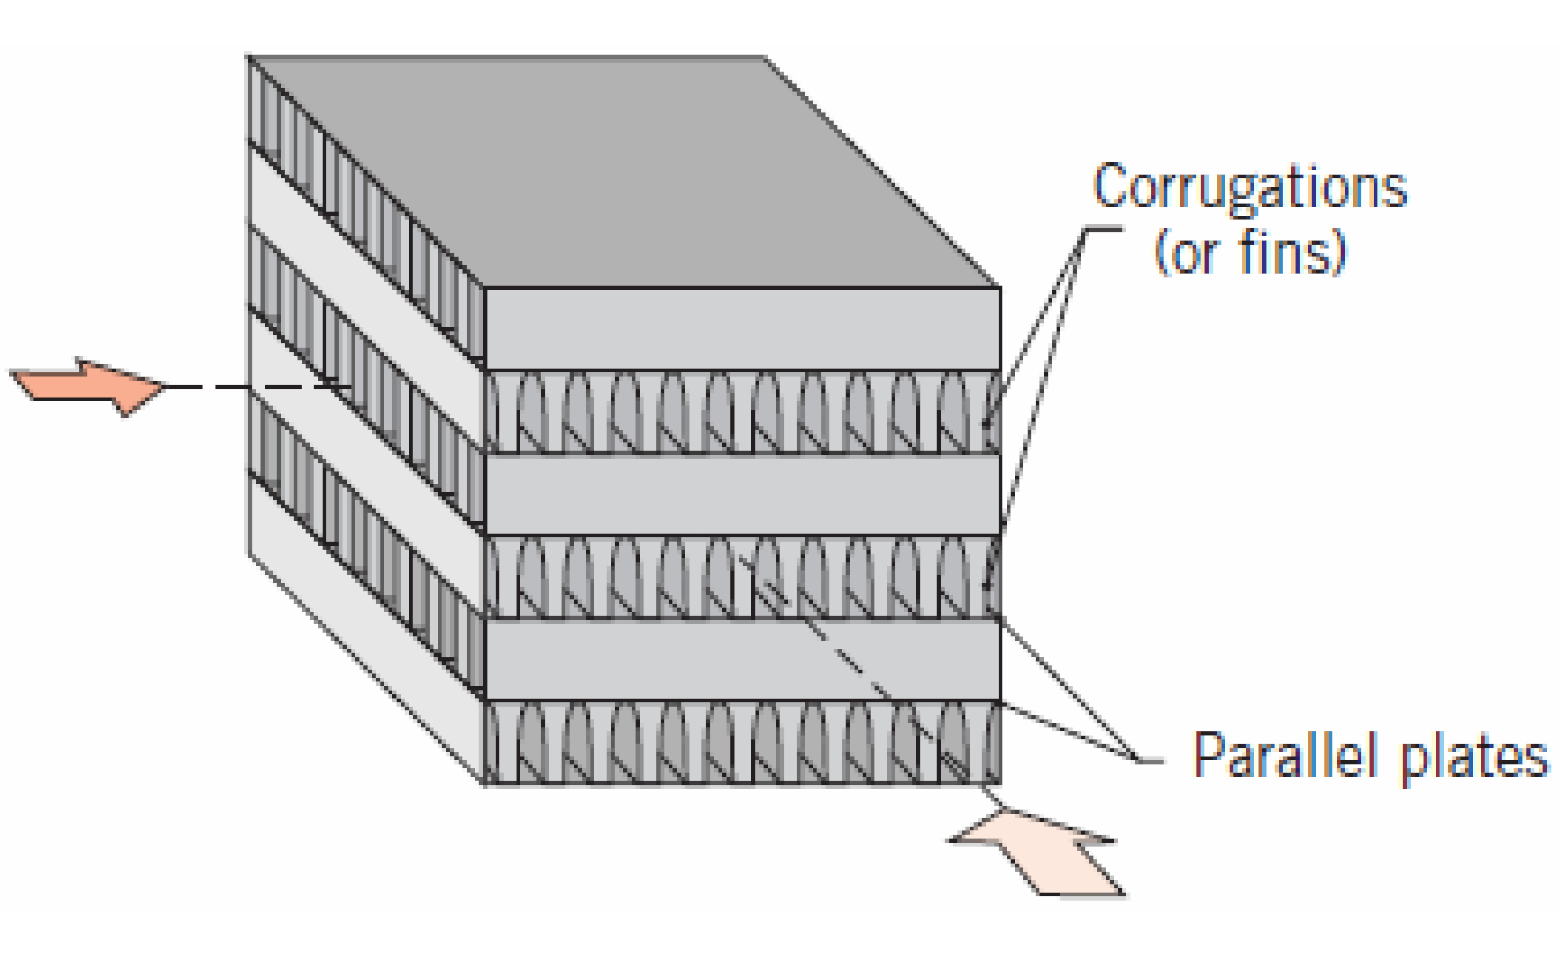
\includegraphics[width=0.4\textwidth]{HX_fin_plate}}\hfill
    \subfloat[HX with fined tubes \cite{Ngendakumana2018}.\label{fig:C4_HX_fin_tube}]
    {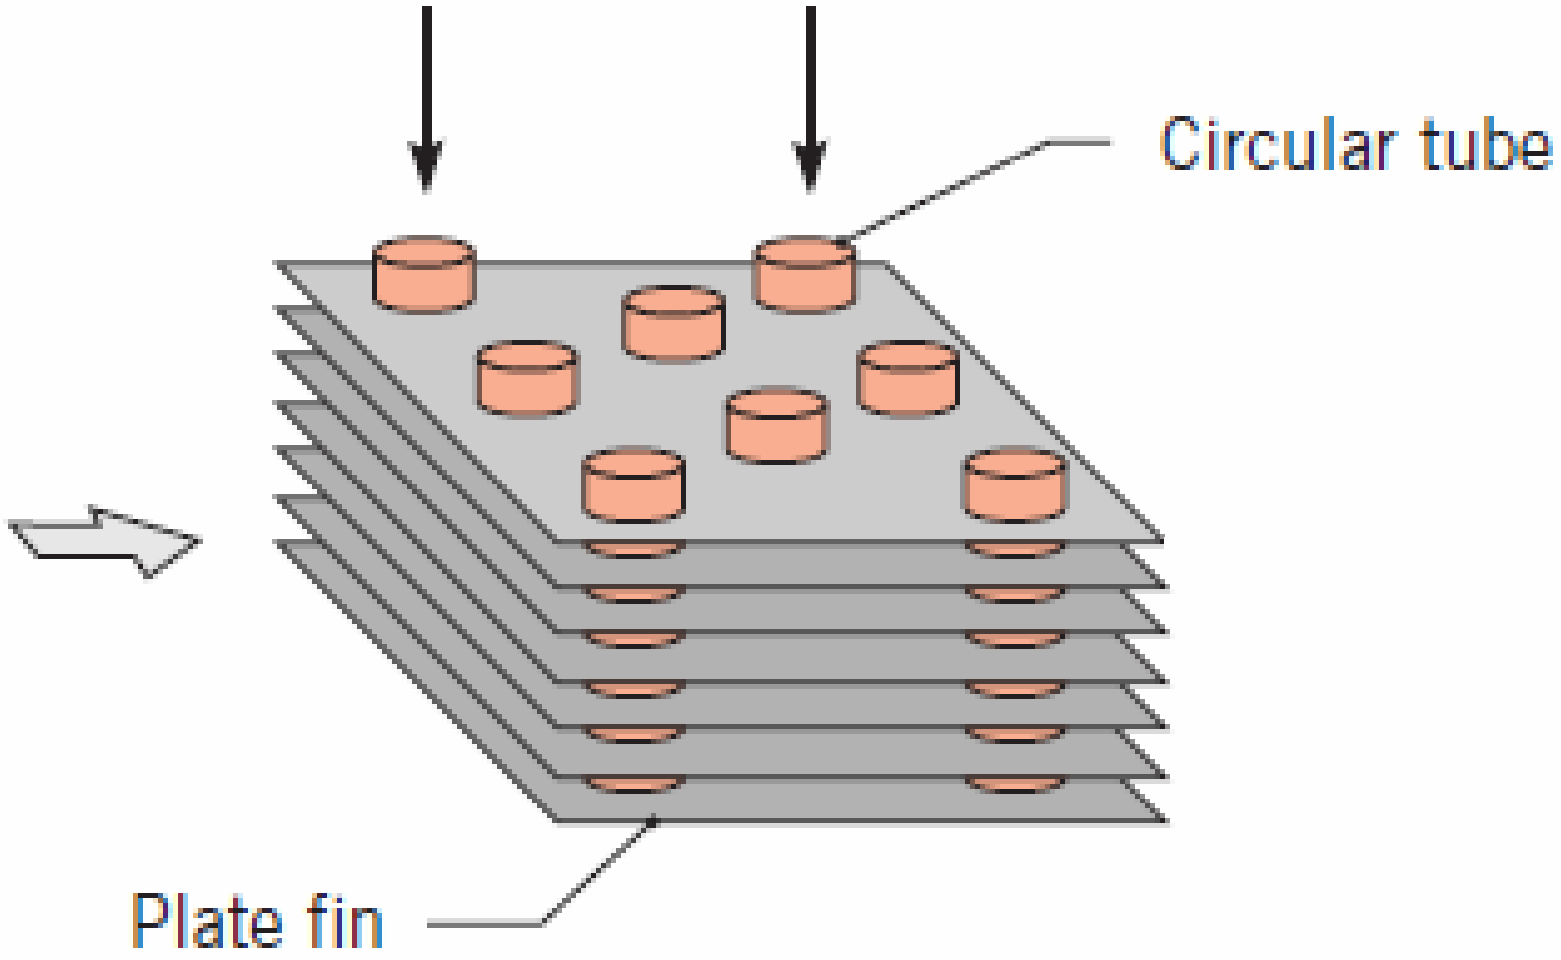
\includegraphics[width=0.4\textwidth]{HX_fin_tube}}\hfill
    \subfloat[Plate heat-exchangers\cite{Ngendakumana2018}.\label{fig:C4_PHE}]
    {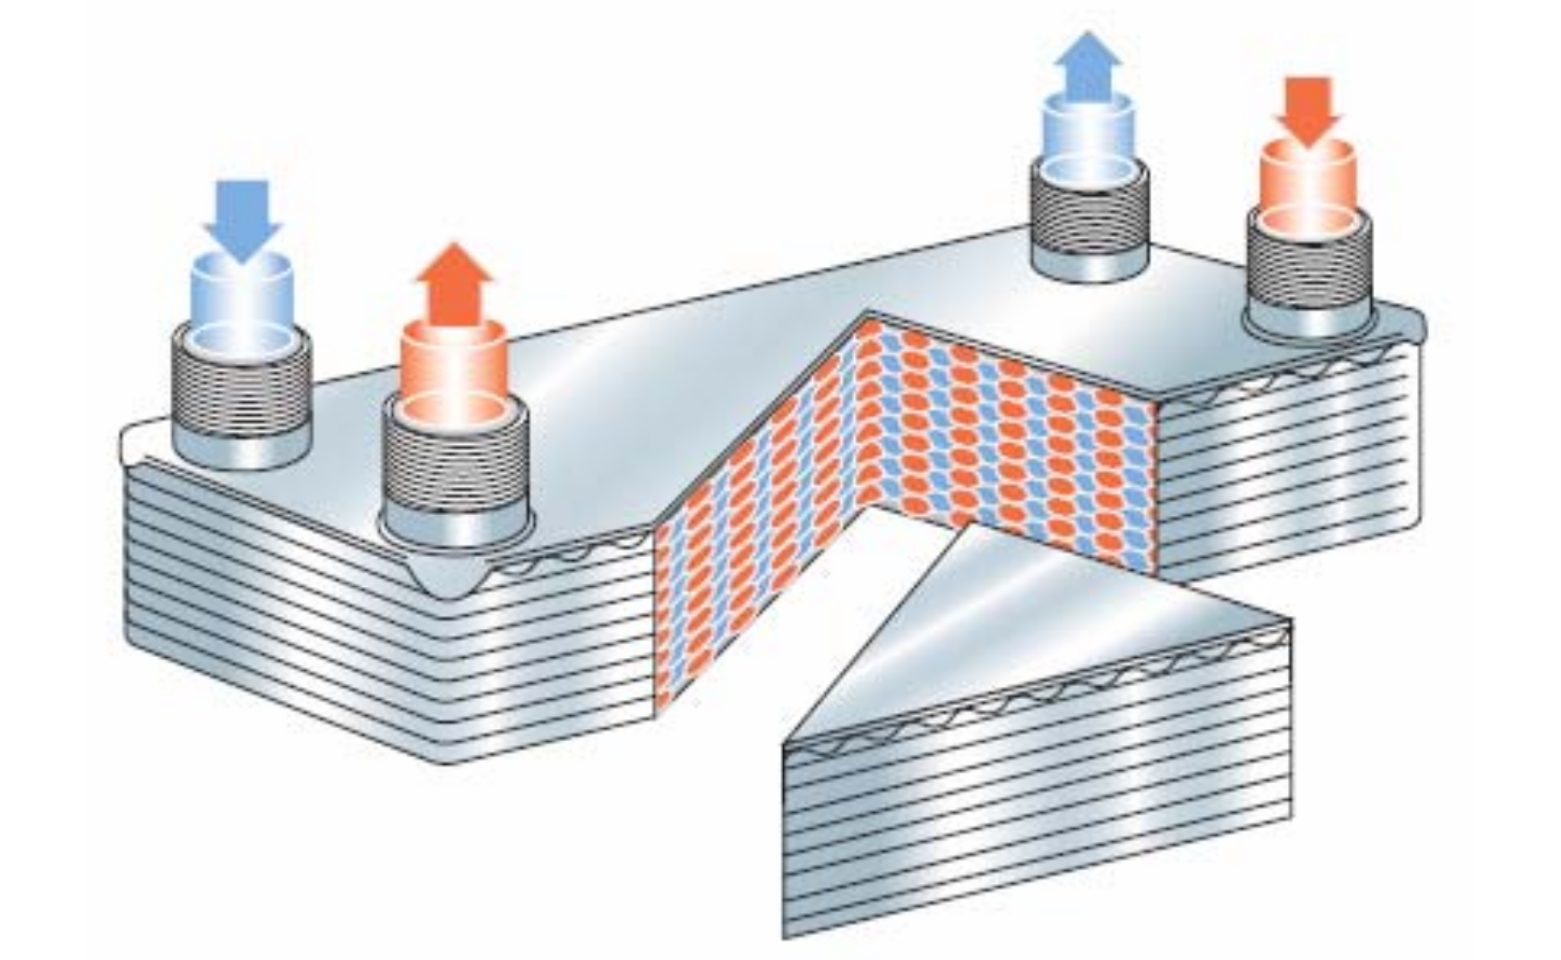
\includegraphics[width=0.4\textwidth]{HX_brased_plate}}
    \caption{HX illustrations.} \label{fig:C4_HX}
\end{figure}

The selected family will highly depends on the type of application that is targeted. Plate heat-exchangers are one of the most compact type of heat-exchangers. This compactness is highly appreciated for any system where the foot print and volume has to be as minimal as possible. However, this is at the cost of more complicated maintenance due the brazing of the plates.

This section will not cover the specificity of these different families. Instead, the main notions which are necessary to characterized the heat transfer between two fluids will be given.

\subsection{Stream configurations}
\quad\ There isn't an unique configuration regarding about the interaction between the hot and cold streams. Indeed, here are the main categories based on flow configurations.

\begin{itemize}
    \setstretch{1}
    \item Parallel flow HX: The two streams go through the heat-exchanger in the same direction (Figure \ref{fig:C4_para_flow}).

    \item Counter flow HX: The two streams go through the heat-exchanger in the opposite direction. This configuration is more frequent than the parallel flow HX due to higher efficiency. However, sometimes the network of piping doesn't permit to install such configuration (Figure \ref{fig:C4_counter_flow}).

    \item Cross flow HX, both fluids unmixed: The flow in the tube does not sees the property of cross flow varying along with the distance traveled. Both flow are unmixed (Figure \ref{fig:C4_cross_flow_unmixed}).
  
    \item Cross flow HX, one fluid mixed: The flow in the tube does not sees the property of cross flow varying along with the distance traveled. The cross flow does not travel inside isolated channels (Figure \ref{fig:C4_cross_flow_1mixed}).
\end{itemize}
\begin{figure}[h]
    \centering
    \begin{subfigure}[b]{0.4\textwidth}
        \centering
        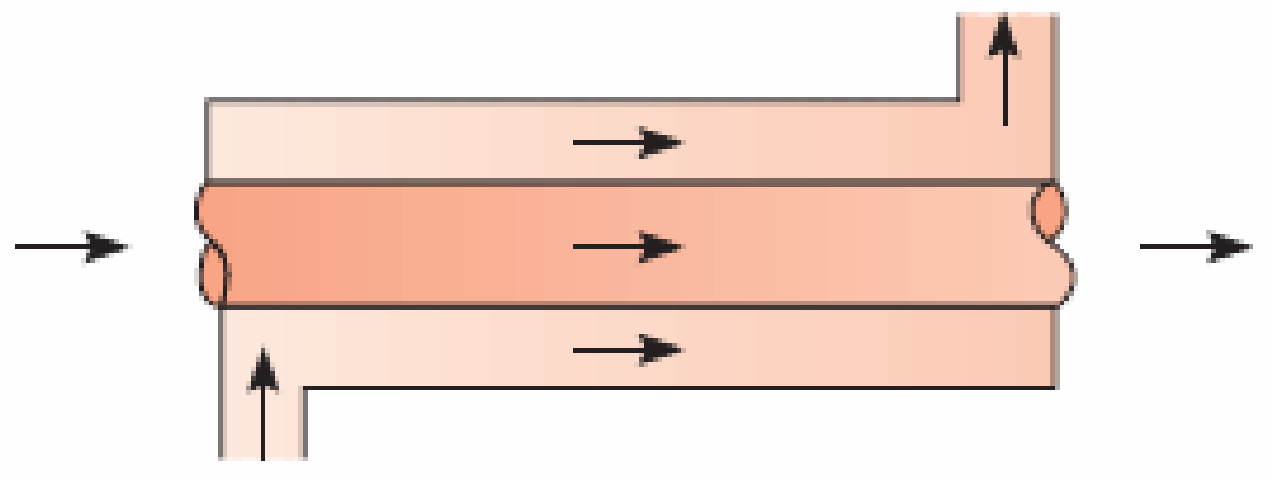
\includegraphics[width=\textwidth]{parallele_flow}
        \caption{Parallel flow heat-exchanger \cite{Ngendakumana2018}.}
        \label{fig:C4_para_flow}
    \end{subfigure}
    \begin{subfigure}[b]{0.4\textwidth}
        \centering
        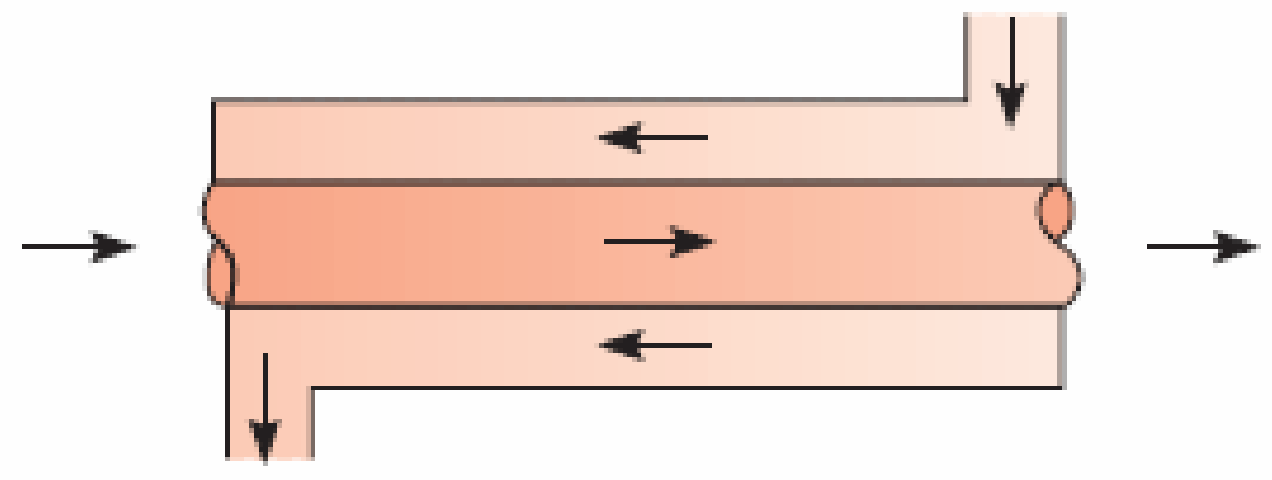
\includegraphics[width=\textwidth]{opposite_flow}
        \caption{Counter flow heat-exchanger \cite{Ngendakumana2018}.}
        \label{fig:C4_counter_flow}
    \end{subfigure}
    \begin{subfigure}[b]{0.4\textwidth}
        \centering
        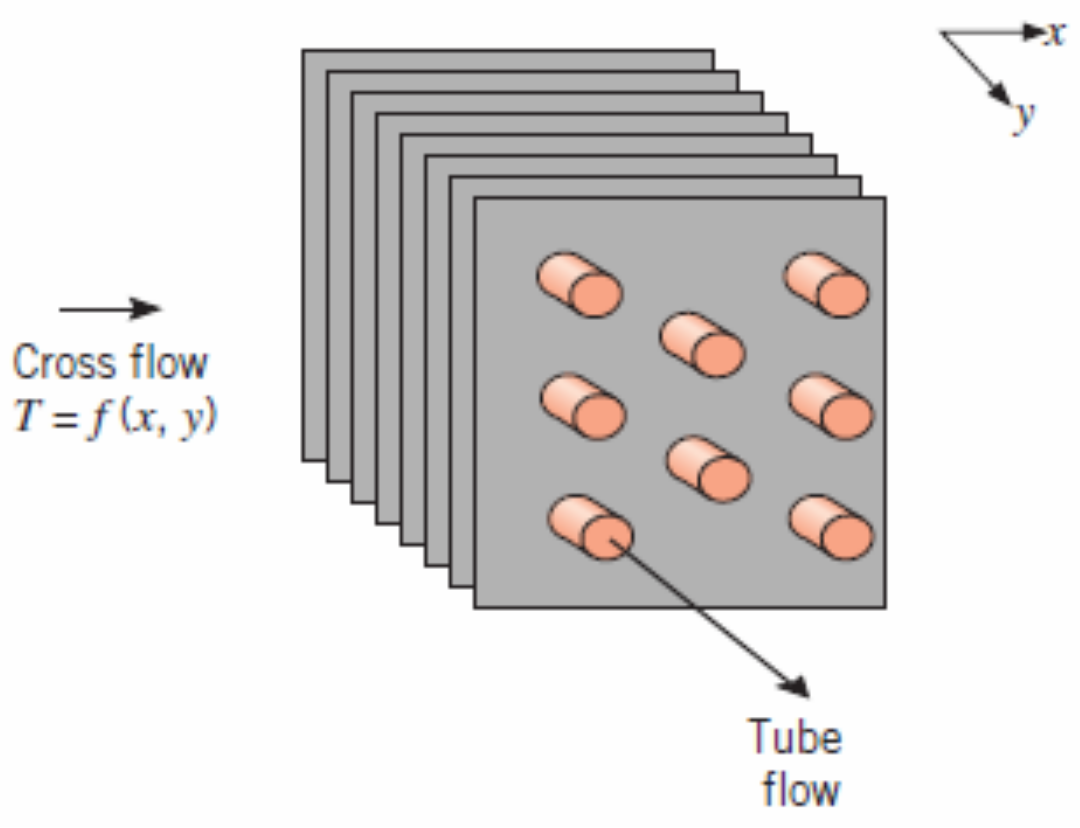
\includegraphics[width=\textwidth]{crossed_flow_non_mixed}
        \caption{Cross flow heat-exchanger, both fluids unmixed \cite{Ngendakumana2018}.}
        \label{fig:C4_cross_flow_unmixed}
    \end{subfigure}
    \begin{subfigure}[b]{0.4\textwidth}
        \centering
        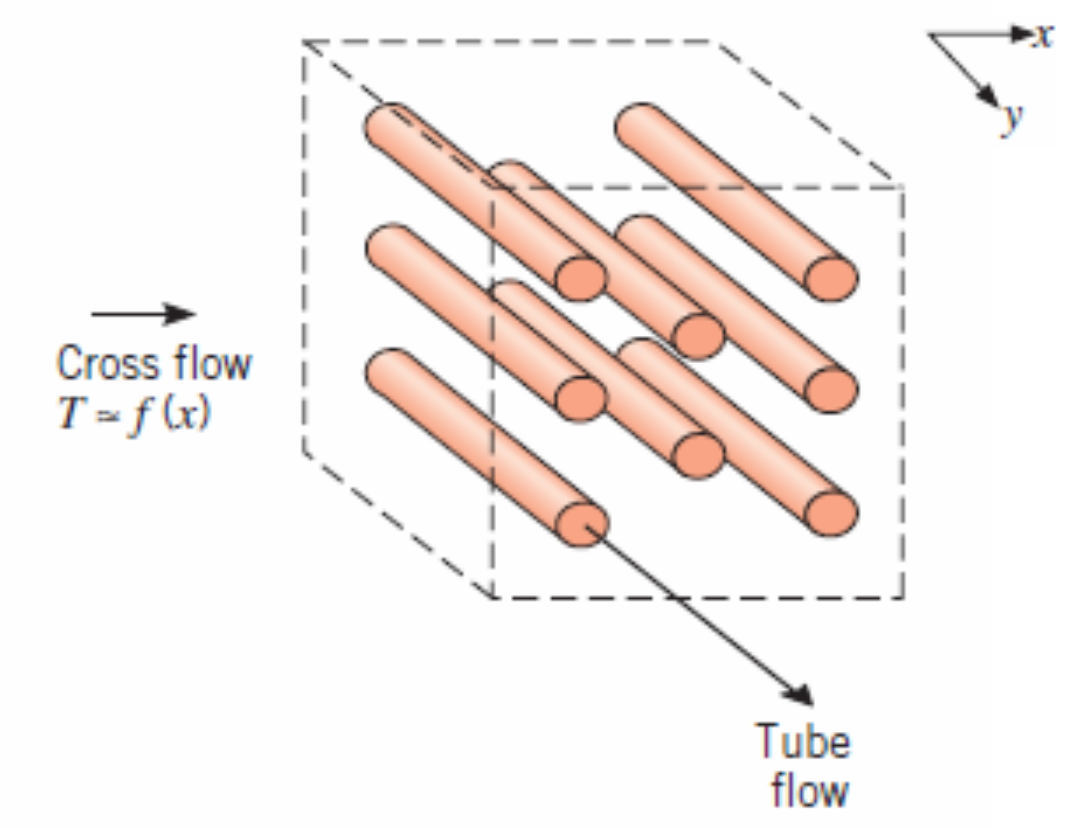
\includegraphics[width=\textwidth]{crossed_flow_one_mixed}
        \caption{Cross flow heat-exchanger, one fluid mixed \cite{Ngendakumana2018}.}
        \label{fig:C4_cross_flow_1mixed}
    \end{subfigure}
    \caption{Configuration Heat-exchangers.} \label{fig:C4_config}
\end{figure}
Considering the parallel and counter flow heat-exchanger, Two temperature differences can be defined based on the temperature profiles (Figure \ref{fig:C4_Tprof}) of both fluids inside the heat-exchanger.

\begin{figure}[h]
    \centering
    \begin{subfigure}[b]{0.4\textwidth}
        \centering
        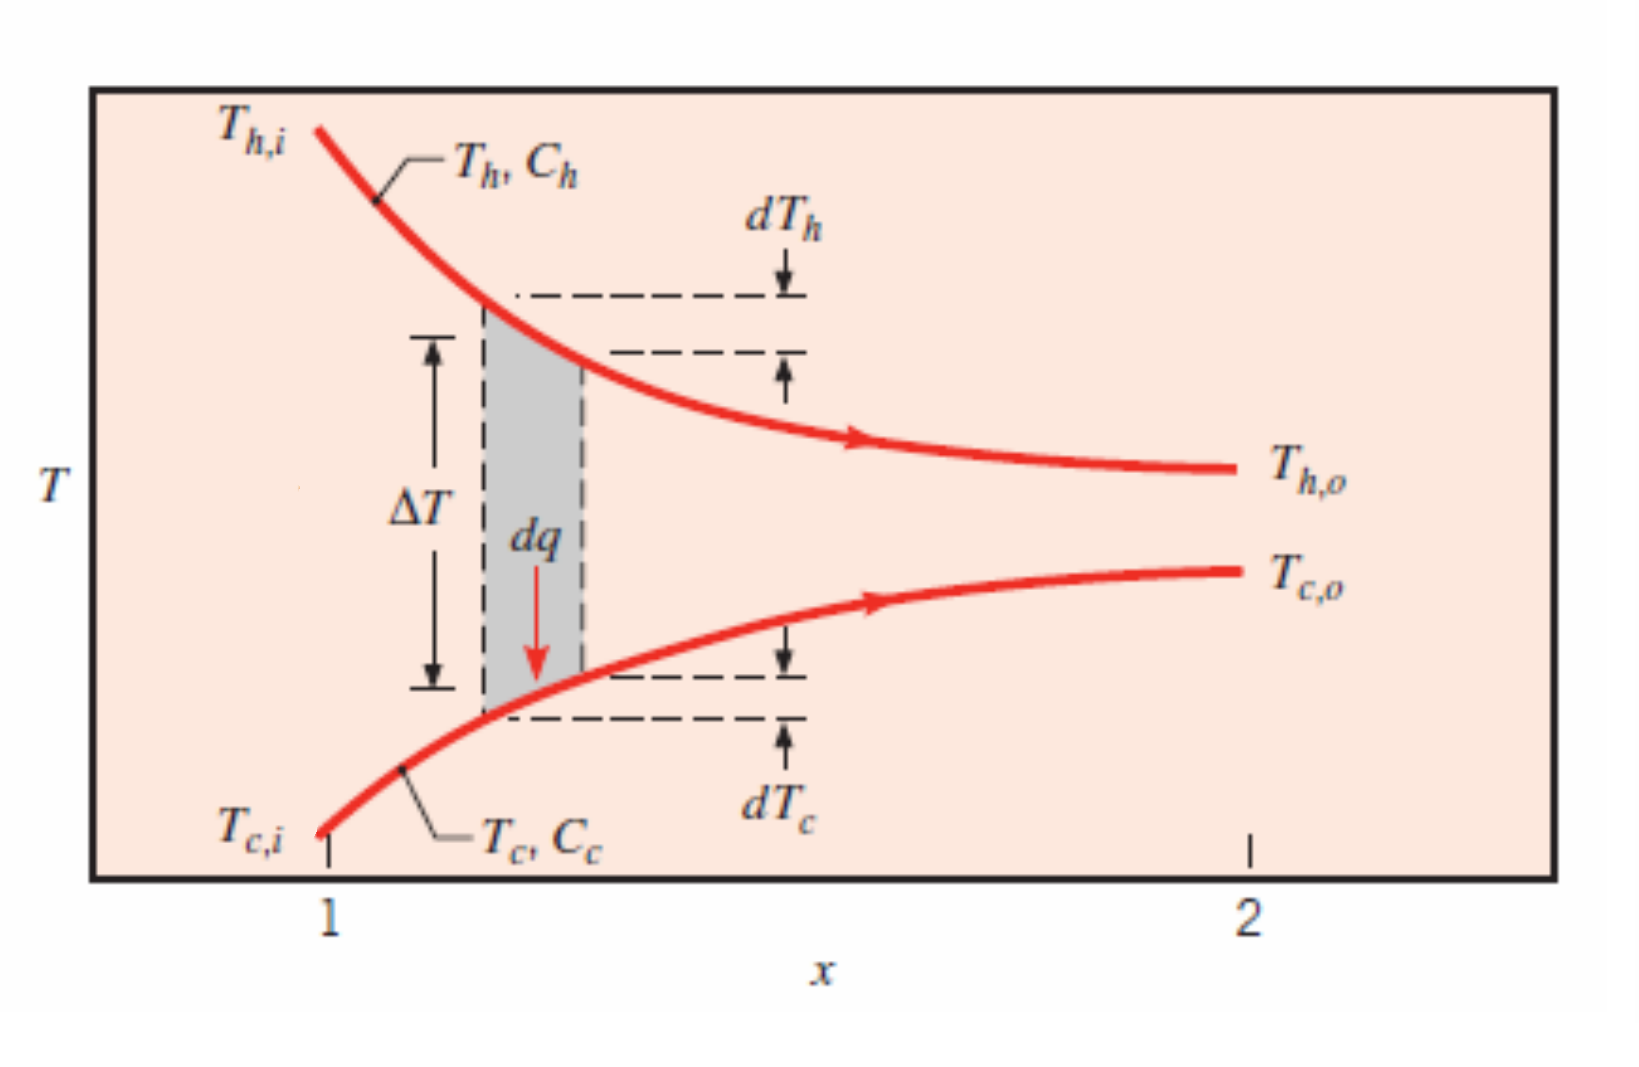
\includegraphics[width=\textwidth]{parallele_flow_T}
        \caption{Temperature profile for parallel flow HX \cite{Ngendakumana2018}.}
        \label{fig:C4_HX_par_flow_T}
    \end{subfigure}
    \begin{subfigure}[b]{0.4\textwidth}
        \centering
        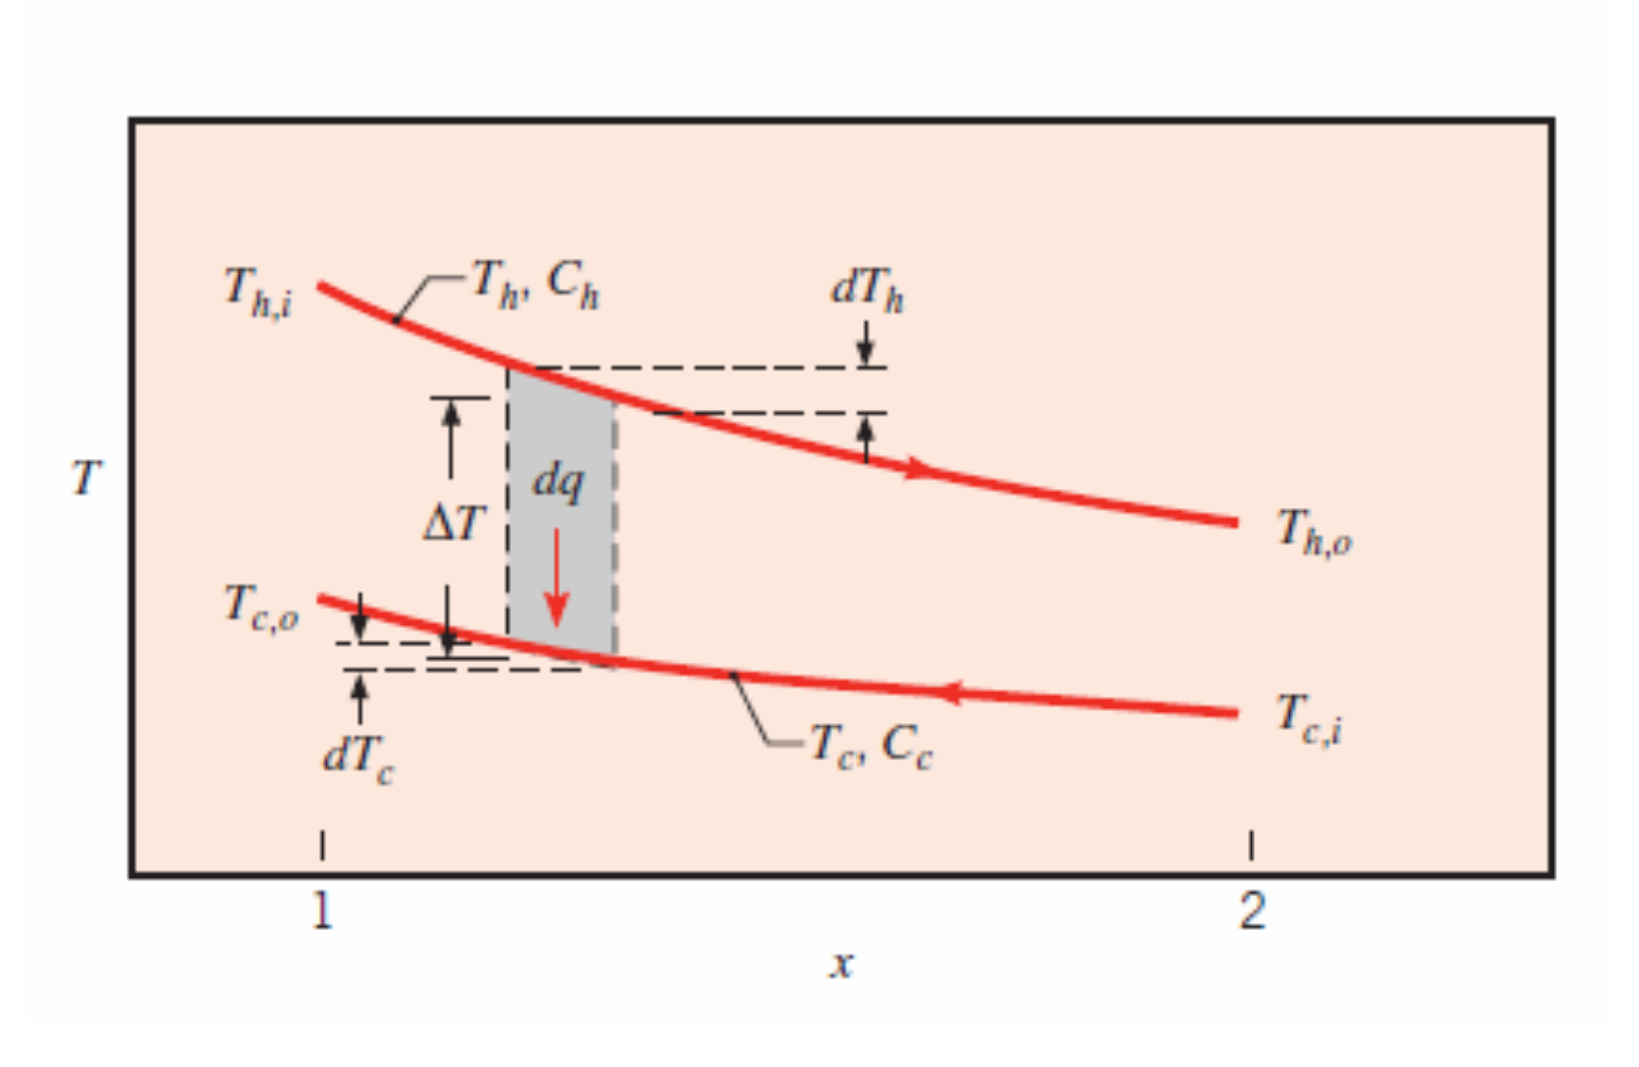
\includegraphics[width=\textwidth]{opposite_flow_T}
        \caption{Temperature profile for counter flow HX \cite{Ngendakumana2018}.}
        \label{fig:C4_HX_opo_flow_T}
    \end{subfigure}
    \caption{Temperature profiles for different stream configurations.}
    \label{fig:C4_Tprof}
\end{figure}

where the subscripts h and c indicate which flow is considered (h:hot; c:cold), and the subscripts i and o refer to the inlet and the outlet of the heat-exchanger.

The first temperature difference \(\Delta T_0\) is defined as being the largest temperature difference between the two flows, regardless the position inside the HX. Thus,

\begin{equation}
    \setstretch{1}
    \Delta T_0 =
    \begin{cases}
        T_{h,i} - T_{c,i} \text{ For the parallel flow} \\
        T_{h,i} - T_{c,o} \text{ For the counter flow}  \\
    \end{cases}\label{eq:C4_DT0}
\end{equation}

The second temperature difference \(\Delta T_L\) corresponds to the smallest temperature difference between the two flows. Thus,

\begin{equation}
    \setstretch{1}
    \Delta T_L =
    \begin{cases}
        T_{h,o} - T_{c,o} \text{ For the parallel flow} \\
        T_{h,o} - T_{c,i} \text{ For the counter flow}  \\
    \end{cases}\label{eq:C4_DTL}
\end{equation}

\subsection{Heat transfer within a heat-exchanger}
\quad\ The heat transfer rate of a heat-exchanger is directly dependent on the nature of the fluids and the heat-exchanger itself. Let's consider the following relation (\ref{eq:C4_Qdot1})
\begin{equation}
    \dot{Q} = \frac{\Delta T_{LM}}{R}= A\cdot U\cdot \Delta T_{LM}\text{ ( in W)}\label{eq:C4_Qdot1}
\end{equation}
where \(A\) is the global surface area of the HX, and \(R\) and \(U\) are the global thermal resistance and transfer coefficient respectively. The \(\Delta T_{LM}\) is called the logarithmic mean temperature difference. It's definition is
\begin{equation}
    \Delta T_{LM} = \frac{\Delta T_0-\Delta T_L}{ln\left(\frac{\Delta T_0}{\Delta T_L}\right)}\label{eq:C4_lmtd}
\end{equation}
with \(ln\) being the neperian logarithm.
\subsubsection{Transfer coefficient}
The general definition for the product \(A\cdot U\) is
\begin{equation}
    \frac{1}{A\cdot U}  = \frac{1}{\eta_{0,c}\cdot h_{conv,c} \cdot A_c} + \frac{F_c}{\eta_{0,c}\cdot A_c} + R_w + \frac{F_h}{\eta_{0,h}\cdot A_h} + \frac{1}{\eta_{0,h}\cdot h_{conv,h} \cdot A_h}\label{eq:C4_AU}
\end{equation}
where \(h_{conv}\) is the convective heat transfer coefficient (in W/m$^2$/K) of the fluid, \(F\) is a degradation factor due to the clogging, \(\eta_0\) is the global efficiency of the surface and \(R_w\) is the wall resistance.

Making the assumption that all the ducts considered in this work are smooth and the flows are turbulent, the convective heat transfer coefficient \(h_{conv}\) is obtained using the formula (\ref{eq:C4_h}).
\begin{equation}
    h_{conv} = Nu \cdot \frac{\lambda_c}{D_t} = 0.023\cdot Re^{0.8}\cdot Pr^{1/3}\frac{\lambda_c}{D_t}\label{eq:C4_h}
\end{equation}
where \(Nu\), \(Re\) and \(Pr\) are the Nusselt, Reynolds and Prandtl number. \(\lambda_c\) is the thermal conductivity (in W/m/K) of the fluid and \(D_t\) is the diameter of the duct\cite{Ngendakumana2018}.

By definition, the Reynolds and Prandtl numbers are defined as follows
\begin{align}
    Re & = \frac{\rho\cdot v\cdot D_h}{\mu}\label{eq:C4_Re} \\
    Pr & = \frac{\mu\cdot c_p}{\lambda_c}\label{eq:C4_Pr}
\end{align}
where \(D_h\) is the hydraulic diameter, \(v\) is the velocity of the flow and \(\mu\) is the dynamic viscosity (in Pa$\cdot$s). The hydraulic diameter and the flow velocity are respectively obtained using the two following relations
\begin{align}
    D_h = \frac{4\cdot A_c}{P_c}\label{eq:C4_Dh}                      \\
    v=\frac{\dot{m}}{\rho\cdot\pi\cdot\frac{D_h^2}{4}}\label{eq:C4_v} \\
\end{align}
with \(A_c\) and \(P_c\) the cross area and perimeter of the duct\cite{Ngendakumana2018}.

Making the assumption that both \(D_h\) and \(D_t\) are equal, let's pose \(D=D_h=D_t\). Therefore, the convective heat transfer coefficient \(h_{conv}\) can be expressed as follows
\begin{equation}
    h_{conv} = 0.0697\cdot \frac{\dot{m}^{4/5}\cdot c_p^{1/3}}{\pi^{4/5}\cdot D^{9/5}}\cdot \frac{\lambda_c^{2/3}}{\mu^{7/15}}
\end{equation}

In the present work, the heat-exchanger that will be used are plate heat-exchangers. For this specific category, the surface dimensions \(A\) for the cold and the hot side are very closed from each others. Also, if the flow considered is only composed of one phase (i.e. only liquid or gaseous), the wall resistance \(R_w\) can be neglected.

If the efficiency \(\eta_0\) are supposed equal for both the hot and the cold side and if the degradation factors \(F\) are neglected, then the heat transfer coefficient \(U\) can be approached by
\begin{equation}
    U \simeq \frac{h_{conv,h}\cdot h_{conv,c}}{h_{conv,h} + h_{conv,c}}\label{eq:C4_AU_prop}
\end{equation}
\subsubsection{LMTD method}
\quad\ In the previous lines, a definition of the heat transfer rate based on the global transfer coefficient. This method is called the LMTD method and requires the knowledge of the geometry of the heat-exchanger.
When the \(\dot{Q}\) has been calculated, the temperatures at the outlet of the heat-exchanger for the cold and hot stream can be computed using the two equations (\ref{eq:C4_ThQ}) and (\ref{eq:C4_TcQ}).

\begin{subequations}
    \setstretch{1}
    \begin{equation}
        \dot{Q} = \dot{m}_h\cdot c_{p,h}\cdot(T_{h,in} - T_{h,out}) =\dot{C}_h\cdot(T_{h,in} - T_{h,out}) \label{eq:C4_ThQ}
    \end{equation}
    \begin{equation}
        \dot{Q} = \dot{m}_c\cdot c_{p,c}\cdot (T_{c,out} - T_{c,in}) =\dot{C}_c\cdot (T_{c,out} - T_{c,in}) \label{eq:C4_TcQ}
    \end{equation}
\end{subequations}

This method requires the knowledge of the inlet and outlet temperatures of both fluids before initiating the computation of the heat transfer rate \(\dot{Q}\) using the relation (\ref{eq:C4_Qdot1}). Therefore, this method needs iteration in the event where these temperatures are not known a priori.

\subsubsection{$\varepsilon$-NTU method}
\quad\ There exists a second method for the evaluation of the heat transfer rate which does not need the outlet temperature of the fluids. First, the maximum heat transfer rate \(\dot{Q}_{max}\) is computed.
\begin{equation}
    \dot{Q}_{max} = \dot{C}_{min}\cdot (T_{h,in} - T_{c,in})
\end{equation}
with \(\dot{C}_{min}=min(\dot{C}_h,\dot{C}_c)\)
Then the heat transfer rate is equal to
\begin{equation}
    \dot{Q} = \varepsilon\cdot\dot{Q}_{max}
\end{equation}
where \(\varepsilon\) is the efficiency of the heat-exchanger. This efficiency is a function of the ratio \(C_r = \frac{\dot{C}_{min}}{\dot{C}_{max}}\), the flow arrangement, and the number of transfer unit NTU defined as being the ratio
\begin{equation}
    \text{NTU} = \frac{A\cdot U}{\dot{C}_{min}}\label{eq:C4_NTU}
\end{equation}

As said, the relations \(\varepsilon(\text{NTU},C_r)\) and \(\text{NTU}(\varepsilon,C_r)\) depend on the heat-exchanger configurations  \cite{GregoryNellis2015}. Here, the type of heat-exchanger used for the modeled Brayton cycle are plate heat-exchanger. Since the flow configuration for this type of heat-exchanger is counter-flow, the associated relation linking the efficiency \(\varepsilon\) to the number of transfer units  NTU is
\begin{equation}
    \varepsilon = \frac{1 - e^{-NTU\cdot \left(1 - C_r\right)}}{1 - C_r\cdot e{-NTU\cdot \left(1 - C_r\right)}}\cite{GregoryNellis2015}
\end{equation}
%%%%%%%%%%%%%%%
%ECRIRE ANNEXE%
%%%%%%%%%%%%%%%

Once the coefficient \(\varepsilon\) computed, the outlet temperatures of the fluids can be obtained using the relations (\ref{eq:C4_ThQ}) and (\ref{eq:C4_TcQ}).

\subsubsection{Rating and sizing problem}
\quad\ The \(\varepsilon\)-NTU method is really useful for solving rating and sizing problems.

On one hand, rating problem are problem that, based on the knowledge of the geometry of the heat-exchanger, evaluates its performance for given inlet temperature for both fluids. For this kind of problem, the NTU is first computed. Then, the efficiency \(\varepsilon\) is derived to allow the calculation of the heat transfer rate.

On the other hand, sizing problems are used for the design of heat-exchanger to provide the wished outlet temperatures. There, the efficiency is first calculated and then the NTU is deduced. Finally, from the equation (\ref{eq:C4_NTU}) the heat transfer area \(A\) can be obtained\cite{Ngendakumana2018}.

A mix of these two types of problems will be used during this work. Indeed, the efficiency \(\varepsilon\) of the heat-exchangers in the system are known for a certain nominal flow rate.    The knowledge of the nominal efficiency provides the required tools to compute the product \(A\cdot U_{nom}\) using the sizing problem methodology.

Then, based on the approximation (\ref{eq:C4_AU_prop}), the \(U\) for the given condition can be obtained since the heat transfer area \(A\) remains unchanged. Finally, the non nominal \(U\) can be used to obtain the of design efficiency \(\varepsilon\). This last step is done through a rating problem.

\section{Piping and pressure drop}
%%%%%%%%%%%%%%%%%%%%%%%%%%%%%%%%%%%
%%%%%                         %%%%%
%%%%%       <<Piping>>        %%%%%
%%%%%                         %%%%%
%%%%%%%%%%%%%%%%%%%%%%%%%%%%%%%%%%%
\quad\ From now, the loss of pressure inside the different elements has not be considered. However, for a system like a gas turbine, the pressure drops have to be as minimal as possible to guaranty that the expanded gas in the turbine is at a pressure as high as possible.

In this work, simple formula will be applied for the pressure drops computation. These one will be computed based on a pressure drop factor \(Dp\) varying from 0 to 1. Then the pressure at the outlet of the component is given by
\begin{equation}
    p_{o} = p_{i}\cdot (1 - Dp)
\end{equation}
where the factor \(Dp\) is different for each component of the system.

Before the present work, the pressure drop factors have been evaluated using computational fluid dynamics (CFD) for a nominal point of operation. Then, it can be demonstrated that the pressure difference \(\Delta p = p_{i} - p_{o}\) is a quadratic function of the mass flow rate \(\dot{m}\). Thus, the pressure losses for any non-nominal points of operation are given by
\begin{equation}
    \Delta p \simeq \Delta p_{nom}\cdot \frac{\dot{m}^2}{\dot{m}^2_{nom}}
\end{equation}

\newpage
%%%%%%%%%%%%%%%%%%%%%%%%%%%%%%%%%
%% Chapitre 5:                 %%
%% Code structure   		   %%
%%%%%%%%%%%%%%%%%%%%%%%%%%%%%%%%%
\graphicspath{{Chapitre_5/Images/}}
\chapter{Brayton cycle modeling - Overview}\label{C5}
%%%%%%%%%%%%%%%%%%%%%%%%%%%%%%%%%%%
%%%%%                         %%%%%
%%%%% Introduction chapitre 5 %%%%%
%%%%%                         %%%%%
%%%%%%%%%%%%%%%%%%%%%%%%%%%%%%%%%%%
\quad\, In the chapter \ref{C4}, the Brayton cycle has been introduced by presenting two configurations. Also, it has been mentioned that many other configurations (illustrated in the annex \ref{annex:Brayton_variant}) exists to cover a large panel of applications. 

This chapter will be devoted to the description of the  Brayton cycle model. This model, will only consider steady state operations. Thus, transient effects like acceleration of the turbomachines or the heating up of the heat-exchangers will not be taken into consideration.

The computer code that will be presented is based on the Python language\citep{van1995python}. The motivations of the usage of this particular computing language, will be given in the beginning of this chapter. Then, the structure of the model itself will be established, followed by the explanation of the implementation of the theoretical aspects saw in chapter \ref{C3}.

\section{Python language}
%%%%%%%%%%%%%%%%%%%%%%%%%%%%%%%%%%%
%%%%%                         %%%%%
%%%%%  <<Python language>>    %%%%%
%%%%%                         %%%%%
%%%%%%%%%%%%%%%%%%%%%%%%%%%%%%%%%%%
\quad\, Python is a computing language that was created by Guido van Rossum at the Centrum Wiskunde \& Informatica (CWI - \url{https://www.cwi.nl}) in the early 1990s. Starting 1995, G. van Rossum continued to work on Python at the Corporation for National Research Initiatives (CNRI - \url{https://www.cnri.reston.va.us/}). Since the very first release, the language was open source. This means that the source code was accessible to anyone. 

From this time, Python progressively gained in popularity, and the community participating to the development of the software didn't stop to grow. Today, this language is used by many companies and for many types of applications. Indeed, this programming language is used for website creation, machine learning, automation, etc. 

Since Python is an open source language, it lives thanks to its community which creates and shares libraries. Indeed, what have already been implemented in the past can be freely used by the other users. Moreover, new users can easily start developing under Python thanks to huge amount of guide and documentation to starting learning about the Python language.

Also, Python is a programming language that allows the object oriented programming. This paradigm consists in the definition of blocks of code (called objects) which are able to interact together through relations, defined in order to solve a given problem. This allows to create computer code that can evolve through the times. 

\section{Structure of the model}
%%%%%%%%%%%%%%%%%%%%%%%%%%%%%%%%%%%
%%%%%                         %%%%%
%%%%% <<Structure of the>>    %%%%%
%%%%%      <<model>>          %%%%%
%%%%%                         %%%%%
%%%%%%%%%%%%%%%%%%%%%%%%%%%%%%%%%%%
\quad\, the previous section shows that Python was a great language due to its huge community and the ability to do oriented object programming. Combined with the fact that Python is free and open source, it has been chosen to program the model developed during this master thesis under the Python language.

The focus of this section is the description of the structure of the computer code itself. As it can be expect from what have been previously said, the program will be composed of multiple blocks that will interact together.

\subsection{Inputs}
\quad\, To start the program, the user has to provide an input file that will contain the required data for the program. The input file is structured as a dictionary\footnote{see \url{https://www.w3schools.com/python/python_dictionaries.asp} for further information} and is composed of three main fields. A template of an input file for the gas turbine configuration is given in the annex \ref{annex:Input_file}.

The first field named "Type" says to the computer code which configuration of the Brayton cycle has to be assess. The possible configurations are listed in Table \ref{tab:C4_inputconfig}.

\begin{longtable}[c]{ll}
\caption{Program input - "Type" field}
\label{tab:C4_inputconfig}\\
\hline
Type - Abbreviation & Type - full name                            \\ \hline
\endfirsthead
%
\multicolumn{2}{c}%
{{\bfseries Table \thetable\ continued from previous page}} \\
\hline
Type - Abbreviation & Type - full name                            \\ \hline
\endhead
%
GT                  & Gas Turbine                                 \\
RGT                 & Regenerative Gas Turbine                    \\
IRGT                & Intercooler-Regenerative Gas Turbine        \\
RHGT                & Regenerative-Reheat Gas Turbine             \\
IHGT                & Intercooler-Reheat Gas Turbine              \\
IRHGT               & Intercooler-Regenerative-Reheat Gas Turbine \\
EFGT                & Externally-Fired Gas Turbine               
\end{longtable} 

These different configurations are described in the annex \ref{Brayton_variant}. 

The second field list all the input data required to initialized the model. The number of variables to be specified at the start of the program depends on the selected configuration. For instance, considering the gas turbine (GT), the inputs required are listed in Table \ref{tab:C4_inputGT}.
\begin{longtable}[c]{llll}
\caption{Input - gas turbine (GT)}
\label{tab:C4_inputGT}\\
\hline
Parameter                                                                             & Symbol         & Parameter                                                                        & Symbol           \\ \hline
\endfirsthead
\multicolumn{4}{c}%
{\tablename\ \thetable\ -- \textit{Continued from previous page}} \\
Parameter                                                                             & Symbol         & Parameter                                                                        & Symbol           \\ \hline
\endhead
\multicolumn{4}{r}{\textit{Continued on next page}} \\
\endfoot
\endlastfoot
%
Reference temperature (°C)                                                            & $T_{ref}$      & \begin{tabular}[c]{@{}l@{}}Combustion chamber\\ efficiency (\%)\end{tabular}     & $\eta_{cc}$      \\
Ambient temperature (°C)                                                              & $T_{amb}$      & \begin{tabular}[c]{@{}l@{}}Shaft mechanical\\ efficiency (\%)\end{tabular}       & $\eta_{shaft}$   \\
Fuel temperature (°C)                                                                 & $T_{fuel}$     & Generator efficiency (\%)                                                        & $\eta_{gen}$     \\
\begin{tabular}[c]{@{}l@{}}Combustion chamber\\ exhaust temperature (°C)\end{tabular} & $T_{cc,ex}$    & \begin{tabular}[c]{@{}l@{}}Compressor isentropic \\ efficiency (\%)\end{tabular} & $\eta_{comp}$    \\
Reference pressure (Pa)                                                               & $p_{ref}$      & \begin{tabular}[c]{@{}l@{}}Turbine isentropic \\ efficiency (\%)\end{tabular}    & $\eta_{t}$       \\
Ambient pressure (Pa)                                                                 & $p_{amb}$      & \begin{tabular}[c]{@{}l@{}}Compressor pressure\\ ratio (-)\end{tabular}          & $P_{comp,ratio}$ \\ \hline
Duct pressure drop (\%)                                                               & $Dp_{duct}$    & Air mass flow rate (kg/s)                                                        & $\dot{m}_{air}$  \\
\begin{tabular}[c]{@{}l@{}}Combustion chamber\\ pressure drop (\%)\end{tabular}       & $Dp_{cc}$      & Nominal mass flow rate (kg/s)                                                    & $\dot{m}_{nom}$  \\
Chimney suction (Pa)                                                                  & $Dp_{chimney}$ & Air factor (-)                                                                   & $\lambda$         \\ \hline
Fuel composition (\%)                                                                 & $Fuel_{char}$  & {\color{PineGreen} Compressor performance map} (.xls/.xlsx) &  $Comp_{excel}$                 \\
Air composition (\%)                                                                  & $Air_{char}$   &{\color{PineGreen} Turbine performance map} (.xls/.xlsx) & $Turb_{excel}$ \\ \hline
{\color{Gray} Rotational speed} (rpm) & $N$ & &\\ \hline
\end{longtable}

The last field named "Selection" is composed of two boolean variables. The first one gives the choice to add a water heat exchanger between the \textit{end} of the cycle and the exhaust. When this variable, named "WHX", is set to \textit{true}, the following inputs as to be added.

\begin{itemize}
\setstretch{1}
\item Water inlet temperature (\degree C): $T_{whx,su,w}$
\item Water outlet temperature (\degree C): $T_{whx,ex,w}$
\item Water inlet pressure (Pa): $p_{whx,su,w}$
\end{itemize}

"MAP" is the second variable. It used to choose whether or not the performance map for the turbomachines (defined as in chapter \ref{C3}). If the variable is set to \textit{true}, the {\color{Gray} gray} field in Table \ref{tab:C4_inputGT} is at least required. Then, depending on the validity of the {\color{PineGreen} pinegreen} fields, the compressor and/or the turbine map(s) will be used in the code. 

When a valid compressor map is given, the variables $\eta_{comp}$ and $P_{comp,ratio}$ are not required to be filled. Indeed, as seen in chapter \ref{C3}, the knowledge of two independent operating variables are sufficient to derived the other variables. In particular, the rotational speed $N$, the air mass flow rate and the inlet state of the compressor are known. Thus, using the relation (\ref{eq:C3_mc}) to obtain the corrected mass flow rate $\dot{m}_{c,comp}$ through the compressor, the compression ratio and the compressor efficiency can be derived.  

Similarly, if a valid turbine map is provided in the inputs, the turbine isentropic efficiency $\eta_{t}$ and the combustion chamber exhaust temperature $T_{cc,ex}$ specified in the inputs will not be used. From the knowledge of the compression ratio, the expansion ratio $P_{turb,ratio}$ can be obtained by computing the pressure drops within the cycle. Then, the efficiency and the corrected mass flow rate $\dot{m}_{c,turb}$ can be derived since two independent variables are known.

The knowledge of both the corrected and \textit{not} corrected mass flow rate through the turbine are sufficient to compute the turbine inlet temperature (TIT). Indeed, the relation (\ref{eq:C3_mc}) from chapter \ref{C3} can be rewritten as followed

\begin{equation}
TIT =T_{ref}\cdot \left(\frac{\dot{m}_c}{\dot{m}}\cdot\frac{p}{p_{ref}}\right)
\end{equation} 

which allows the computation of the turbine inlet temperature.
\newpage
\subsection{Flow chart of the model}
\quad\,  The previous section detailed the the structure of the input file to be provided at the start of the program. Once provided, the program will first read the "Type" field to select the desired configuration. If the configuration is contained in the database of the program, the associated model will be created.
\begin{wrapfigure}{l}{0.45\linewidth}
\centering
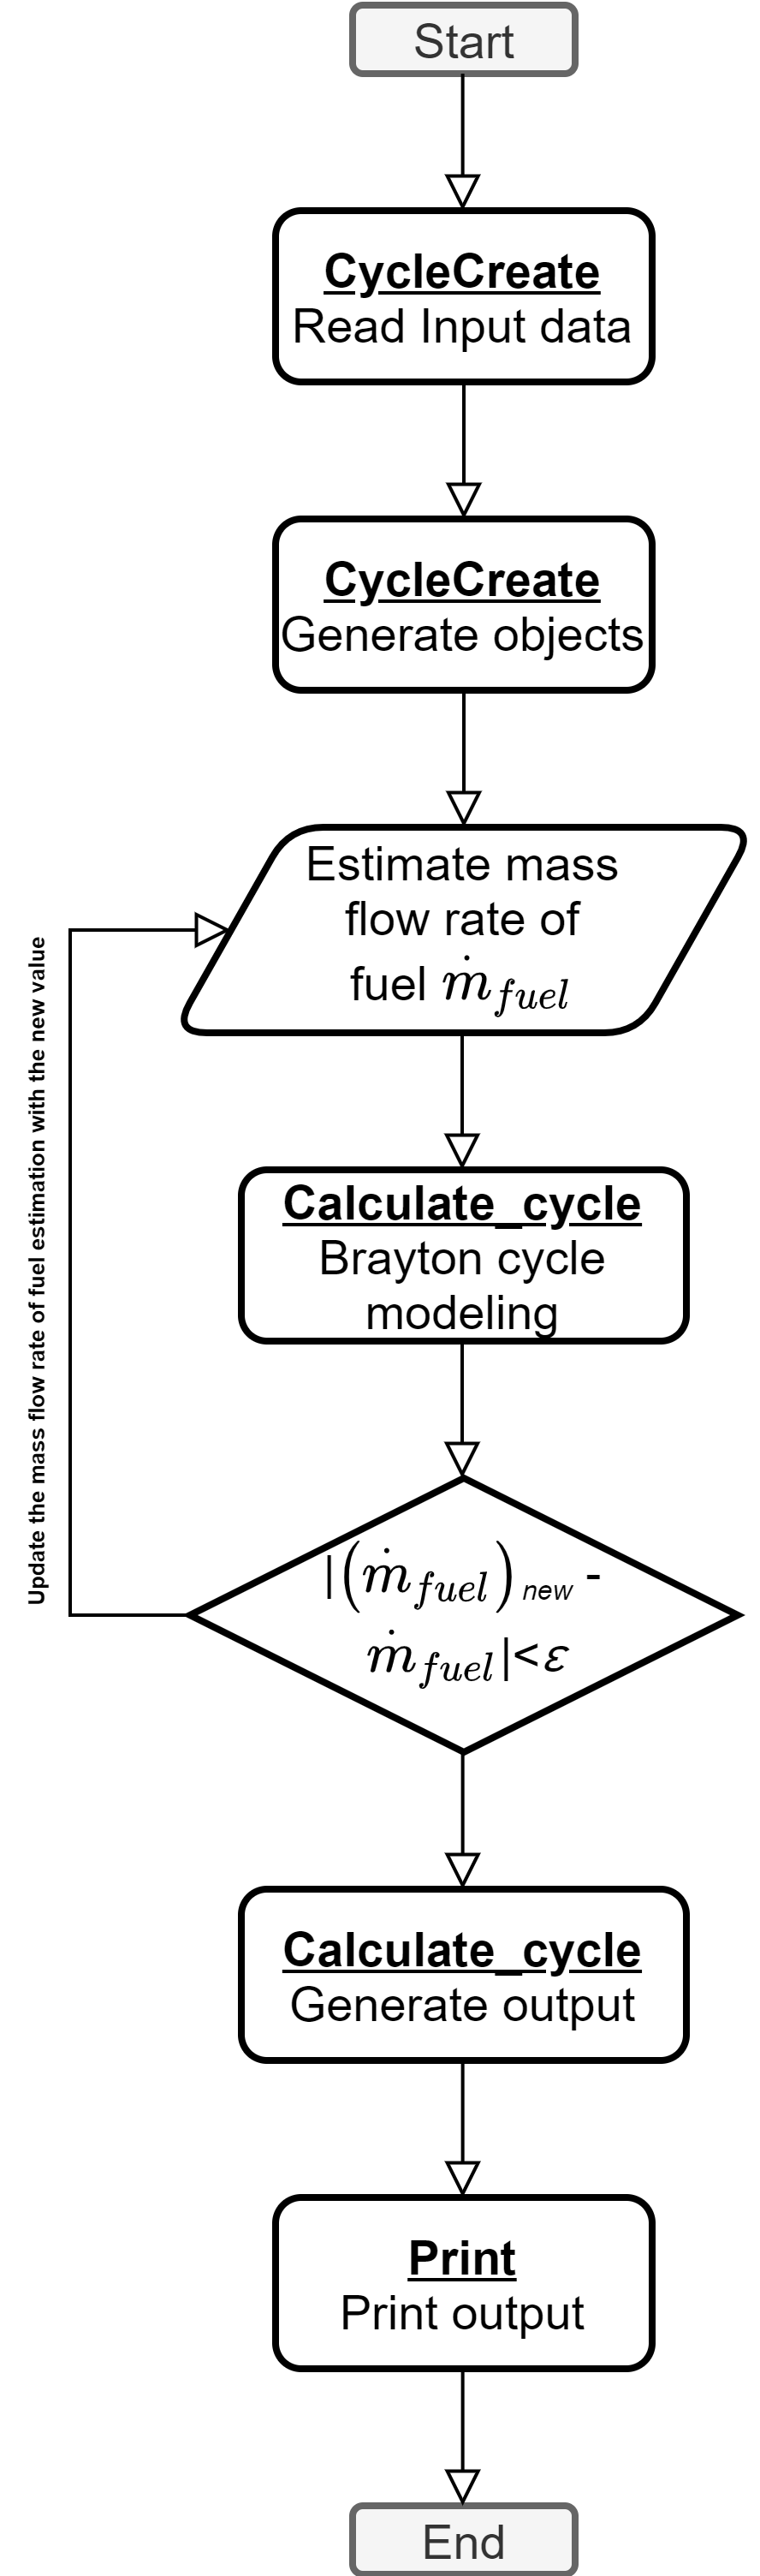
\includegraphics{Flow_chart.png}
\caption{Flow chart of the Brayton cycle model}
\label{fig:C5_flowchart}
\end{wrapfigure}
The second step consists in the reading and storage of the input data from the input file. Then, a restructuring of the input is performed to be understood by the model. This extraction of data is performed regarding to value of the variables within the field "Selection".

When all the required inputs are loaded, the program starts the model. To initiate the assessment of the performance of the selected cycle, a initial guess on the mass flow rate of fuel $\dot{m}_{fuel}$ is realized. Then, the model \textit{travels} along the cycle by calling the objects associated to the real components. 
After having gone through the combustion chamber(s), the mass flow rate of fuel is re-evaluated to update the initial guess. If the change is smaller than $\varepsilon$, the model escapes the loop. Otherwise, new passages are performed until no noticeable change of the mass flow rate value.
   
Finally, outputs are generated based on the assessed cycle. Among these, the temperature, pressure, enthalpy, and density at each state of the cycle are specified. The fuel mass flow rate is also provided to the user along with the thermal efficiency of the cycle and the power consumed and produced. 

This structure is followed for every selected configurations. The flow chart on Figure \ref{fig:C5_flowchart} graphically illustrates the structure of the model from the reading of the inputs to the generation of the outputs.\\ \newpage

As it has been presented, the main structure of the program is relatively linear without many branches. This linear scheme allows a rapid comprehension of how the program works from the outside. However, when considering the calls of the objects in the \textsc{Calculate\_cycle} function, the structure becomes more complex. 

Thus, this main function relies on objects to live within the program.  Among these objects, two categories, namely the \textbf{static} and \textbf{non-static} object, can be defined.

The first category called \textbf{static} objects are the objects associated to the thermodynamic components (compressor, turbine,etc...). These objects are called statics because each of the components will not change of position in the cycle once the latter is defined. \\

Then, there are the objects representing the fluids involved in cycle. These \textbf{non static} objects will live the thermodynamic cycle by going through the different components.

For a Brayton cycle, the modeled fluids are typically air, fuel, exhaust gas, and sometimes water (if there is any water heat exchanger). This explicit definition for each of these fluids is useful. Indeed, it allows to create a more flexible model since the modification of one fluid composition has only to be performed while defining the associated object. 

The next chapter will present the implementation method of each thermodynamic components. For each of those, the functions involved will be defined and explained. Also, some links with the theoretical notions seen in chapters \ref{C2} and \ref{C3} will be created.





 
\newpage
%%%%%%%%%%%%%%%%%%%%%%%%%%%%%%%%%
%% Chapitre 6:                 %%
%% Brayton cycle modeling      %%
%%%%%%%%%%%%%%%%%%%%%%%%%%%%%%%%%
\graphicspath{{Chapitre_6/Images/}}
\chapter{Model overview}\label{C6}
%%%%%%%%%%%%%%%%%%%%%%%%%%%%%%%%%%%
%%%%%                         %%%%%
%%%%% Introduction chapitre 5 %%%%%
%%%%%                         %%%%%
%%%%%%%%%%%%%%%%%%%%%%%%%%%%%%%%%%%
\quad\, In the chapter \ref{C5}, the Brayton cycle has been introduced by presenting two configurations. Also, it has been mentioned that many other configurations (illustrated in the annex \ref{annex:Brayton_variant}) exists to cover a large panel of applications. 

This chapter will be devoted to the description of the  Brayton cycle model. This model, will only consider steady state operations. Thus, transient effects like acceleration of the turbomachines or the heating up of the heat-exchangers will not be taken into consideration.
 

\section{Python language}
%%%%%%%%%%%%%%%%%%%%%%%%%%%%%%%%%%%
%%%%%                         %%%%%
%%%%%  <<Python language>>    %%%%%
%%%%%                         %%%%%
%%%%%%%%%%%%%%%%%%%%%%%%%%%%%%%%%%%
\quad\, Python is a computing language that was created by Guido van Rossum at the Centrum Wiskunde \& Informatica (CWI - \url{https://www.cwi.nl}) in the early 1990s. Starting 1995, G. van Rossum continued to work on Python at the Corporation for National Research Initiatives (CNRI - \url{https://www.cnri.reston.va.us/}). Since the very first release, the language was open source. This means that the source code was accessible to anyone. 

From this time, Python progressively gained in popularity, and the community participating to the development of the software didn't stop to grow. Today, this language is used by many companies and for many types of applications. Indeed, this programming language is used for website creation, machine learning, automation, etc. 

Since Python is an open source language, it lives thanks to its community which creates and shares libraries. Indeed, what have already been implemented in the past can be freely used by the other users. Moreover, new users can easily start developing under Python thanks to huge amount of guide and documentation to starting learning about the Python language.

Also, Python is a programming language that allows the object oriented programming. This paradigm consists in the definition of blocks of code (called objects) which are able to interact together through relations, defined in order to solve a given problem. This allows to create computer code that can evolve through the times. 

\section{Model structure}
%%%%%%%%%%%%%%%%%%%%%%%%%%%%%%%%%%%
%%%%%                         %%%%%
%%%%% <<Structure of the>>    %%%%%
%%%%%      <<model>>          %%%%%
%%%%%                         %%%%%
%%%%%%%%%%%%%%%%%%%%%%%%%%%%%%%%%%%
\quad\, the previous section shows that Python was a great language due to its huge community and the ability to do oriented object programming. Combined with the fact that Python is free and open source, it has been chosen to program the model developed during this master thesis under the Python language.

The focus of this section is the description of the structure of the computer code itself. As it can be expect from what have been previously said, the program will be composed of multiple blocks that will interact together.

\subsection{Inputs}
\quad\, To start the program, the user has to provide an input file that will contain the required data for the program. The input file is structured as a dictionary\footnote{see \url{https://www.w3schools.com/python/python_dictionaries.asp} for further information} and is composed of three main fields. A template of an input file for the gas turbine configuration is given in the annex \ref{annex:Input_file}.

The first field named "Type" says to the computer code which configuration of the Brayton cycle has to be assess. The possible configurations are listed in Table \ref{tab:C6_inputconfig}.

\begin{longtable}[c]{ll}
\caption{Program input - "Type" field}
\label{tab:C6_inputconfig}\\
\toprule
\textbf{Type - Acronym} & \textbf{Type - Name}                   \\* \midrule
\endfirsthead
%
\endhead
%
\bottomrule
\endfoot
%
\endlastfoot
%
GT                           & Gas Turbine                                 \\
RGT                          & Regenerative Gas Turbine                    \\
IRGT                         & Intercooler-Regenerative Gas Turbine        \\
RHGT                         & Regenerative-Reheat Gas Turbine             \\
IHGT                         & Intercooler-Reheat Gas Turbine              \\
IRHGT                        & Intercooler-Regenerative-Reheat Gas Turbine \\
EFGT                         & Externally-Fired Gas Turbine                \\* \bottomrule
\end{longtable}

These different configurations are described in the annex \ref{annex:Brayton_variant}. 

The second field list all the input data required to initialized the model. The number of variables to be specified at the start of the program depends on the selected configuration. For instance, considering the gas turbine (GT), the inputs required are listed in Table \ref{tab:C6_inputGT}.
\begin{longtable}[c]{ll|ll}
\caption{Input - gas turbine (GT)}
\label{tab:C6_inputGT}\\
\toprule
\textbf{Inputs - Name}                                                                          & \textbf{Inputs - Abbreviation} & \textbf{Inputs - Name}                                                                                          & \textbf{Inputs - Abbreviation} \\* \midrule
\endfirsthead
%
\endhead
%
\bottomrule
\endfoot
%
\endlastfoot
%
\begin{tabular}[c]{@{}l@{}}Reference \\ temperature (°C)\end{tabular}                  & $T_{ref}$             & \begin{tabular}[c]{@{}l@{}}Combustion chamber \\ efficiency (\%)\end{tabular}                          & $\eta_{cc}$           \\
\begin{tabular}[c]{@{}l@{}}Ambient \\ temperature (°C)\end{tabular}                    & $T_{amb}$             & \begin{tabular}[c]{@{}l@{}}Shaft mechanical \\ efficiency (\%)\end{tabular}                            & $\eta_{shaft}$        \\
\begin{tabular}[c]{@{}l@{}}Fuel \\ temperature (°C)\end{tabular}                       & $T_{fuel}$            & \begin{tabular}[c]{@{}l@{}}Generator \\ efficiency (\%)\end{tabular}                                   & $\eta_{gen}$          \\
\begin{tabular}[c]{@{}l@{}}Combustion chamber \\ exhaust temperature (°C)\end{tabular} & $T_{cc,ex}$           & \begin{tabular}[c]{@{}l@{}}Compressor isentropic \\ efficiency (\%)\end{tabular}                       & $\eta_{comp}$         \\
\begin{tabular}[c]{@{}l@{}}Reference \\ pressure (Pa)\end{tabular}                     & $p_{ref}$             & \begin{tabular}[c]{@{}l@{}}Turbine isentropic \\ efficiency (\%)\end{tabular}                          & $\eta_{t}$            \\
\begin{tabular}[c]{@{}l@{}}Ambient \\ pressure (Pa)\end{tabular}                       & $p_{amb}$             & \begin{tabular}[c]{@{}l@{}}Compressor \\ pressure ratio (-)\end{tabular}                               & $P_{comp,ratio}$      \\
\begin{tabular}[c]{@{}l@{}}Duct \\ pressure drop (\%)\end{tabular}                     & $Dp_{duct}$           & \begin{tabular}[c]{@{}l@{}}Air mass \\ flow rate (kg/s)\end{tabular}                                   & $\dot{m}_{air}$       \\
\begin{tabular}[c]{@{}l@{}}Combustion chamber \\ pressure drop (\%)\end{tabular}       & $Dp_{cc}$             & \begin{tabular}[c]{@{}l@{}}Nominal mass \\ flow rate (kg/s)\end{tabular}                               & $\dot{m}_{nom}$       \\
Chimney suction (Pa)                                                                   & $Dp_{chimney}$        & Air factor (-)                                                                                         & $\lambda$             \\
Fuel composition (\%)                                                                  & $Fuel_{char}$         & \begin{tabular}[c]{@{}l@{}}{\color{PineGreen}{Compressor}} \\ {\color{PineGreen}{performance map}} (.xls/.xlsx)\end{tabular} & $Comp_{excel}$        \\
Air composition (\%)                                                                   & $Air_{char}$          & \begin{tabular}[c]{@{}l@{}}{\color{PineGreen}{Turbine}} \\ {\color{PineGreen}{performance map}} (.xls/.xlsx)\end{tabular}    & $Turb_{excel}$        \\
{\color{Gray} Rotational speed} (rpm)                                                  & $N$                   &                                                                                                        &                       \\* \bottomrule
\end{longtable}

The last field named "Selection" is composed of two boolean variables. The first one gives the choice to add a water heat exchanger between the \textit{end} of the cycle and the exhaust. When this variable, named "WHX", is set to \textit{true}, the following inputs as to be added.

\begin{itemize}
\setstretch{1}
\item Water inlet temperature (\degree C): $T_{whx,su,w}$
\item Water outlet temperature (\degree C): $T_{whx,ex,w}$
\item Water inlet pressure (Pa): $p_{whx,su,w}$
\end{itemize}

"MAP" is the second variable. It used to choose whether or not the performance map for the turbomachines (defined as in chapter \ref{C4}). If the variable is set to \textit{true}, the {\color{Gray} gray} field in Table \ref{tab:C6_inputGT} is at least required. Then, depending on the validity of the {\color{PineGreen} pinegreen} fields, the compressor and/or the turbine map(s) will be used in the code. 

When a valid compressor map is given, the variables $\eta_{comp}$ and $P_{comp,ratio}$ are not required to be filled. Indeed, as seen in chapter \ref{C4}, the knowledge of two independent operating variables are sufficient to derived the other variables. In particular, the rotational speed $N$, the air mass flow rate and the inlet state of the compressor are known. Thus, using the relation (\ref{eq:C4_mc}) to obtain the corrected mass flow rate $\dot{m}_{c,comp}$ through the compressor, the compression ratio and the compressor efficiency can be derived.  

Similarly, if a valid turbine map is provided in the inputs, the turbine isentropic efficiency $\eta_{t}$ and the combustion chamber exhaust temperature $T_{cc,ex}$ specified in the inputs will not be used. From the knowledge of the compression ratio, the expansion ratio $P_{turb,ratio}$ can be obtained by computing the pressure drops within the cycle. Then, the efficiency and the corrected mass flow rate $\dot{m}_{c,turb}$ can be derived since two independent variables are known.

The knowledge of both the corrected and \textit{not} corrected mass flow rate through the turbine are sufficient to compute the turbine inlet temperature (TIT). Indeed, the relation (\ref{eq:C4_mc}) from chapter \ref{C4} can be rewritten as followed

\begin{equation}
    \setstretch{1}
TIT =T_{ref}\cdot \left(\frac{\dot{m}_c}{\dot{m}}\cdot\frac{p}{p_{ref}}\right)
\end{equation} 

which allows the computation of the turbine inlet temperature.
\newpage
\subsection{Flow chart of the model}
\quad\,  The previous section detailed the the structure of the input file to be provided at the start of the program. Once provided, the program will first read the "Type" field to select the desired configuration. If the configuration is contained in the database of the program, the associated model will be created.
\begin{wrapfigure}{l}{0.42\linewidth}
\centering
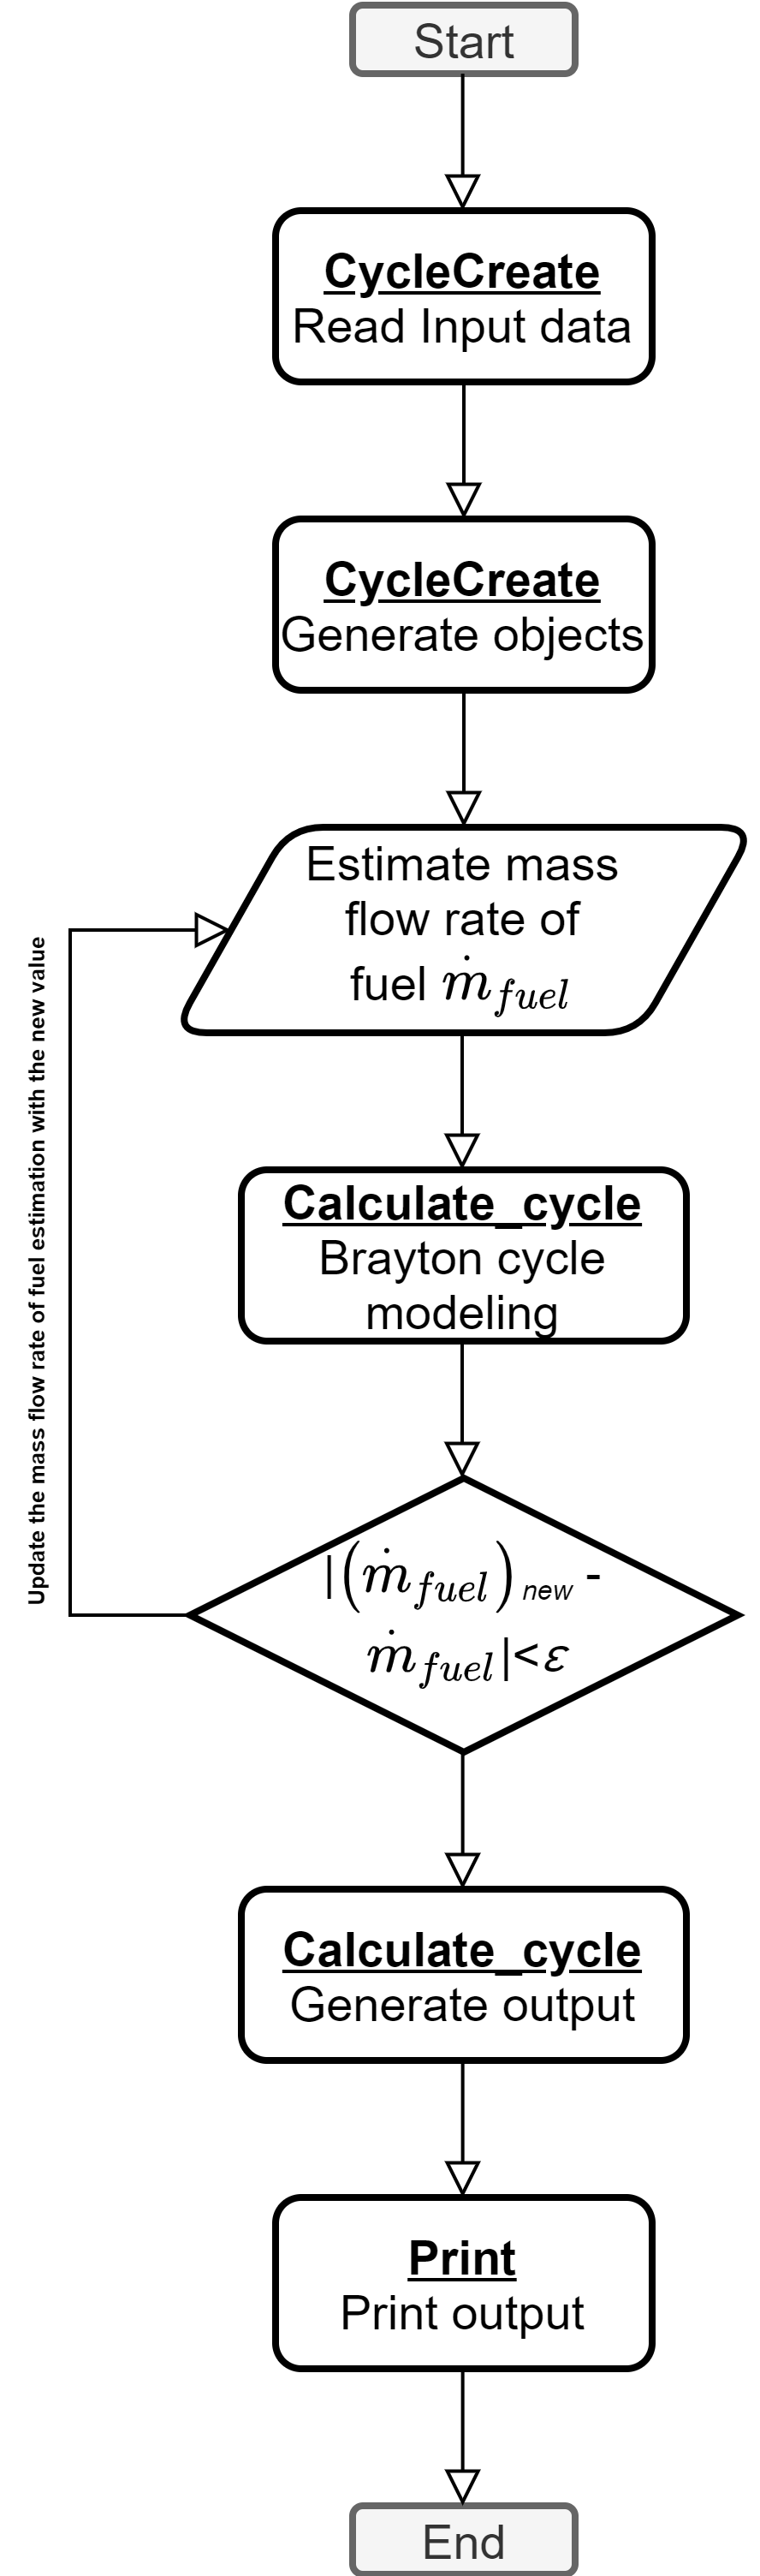
\includegraphics{Flow_chart.png}
\caption{Flow chart of the Brayton cycle model}
\label{fig:C6_flowchart}
\end{wrapfigure}
The second step consists in the reading and storage of the input data from the input file. Then, a restructuring of the input is performed to be understood by the model. This extraction of data is performed regarding to value of the variables within the field "Selection".

When all the required inputs are loaded, the program starts the model. To initiate the assessment of the performance of the selected cycle, a initial guess on the mass flow rate of fuel $\dot{m}_{fuel}$ is realized. Then, the model \textit{travels} along the cycle by calling the objects associated to the real components. 
After having gone through the combustion chamber(s), the mass flow rate of fuel is re-evaluated to update the initial guess. If the change is smaller than $\varepsilon$, the model escapes the loop. Otherwise, new passages are performed until no noticeable change of the mass flow rate value.
   
Finally, outputs are generated based on the assessed cycle. Among these, the temperature, pressure, enthalpy, and density at each state of the cycle are specified. The fuel mass flow rate is also provided to the user along with the thermal efficiency of the cycle and the power consumed and produced. 

This structure is followed for every selected configurations. The flow chart on Figure \ref{fig:C6_flowchart} graphically illustrates the structure of the model from the reading of the inputs to the generation of the outputs.\clearpage

As it has been presented, the main structure of the program is relatively linear without many branches. This linear scheme allows a rapid comprehension of how the program works from the outside. However, when considering the calls of the objects in the ''Calculate\_cycle'' function, the structure becomes more complex. 

Thus, this main function relies on objects to live within the program.  Among these objects, two categories, namely the \textbf{static} and \textbf{non-static} object, can be defined.

The first category called \textbf{static} objects are the objects associated to the thermodynamic components (compressor, turbine,etc...). These objects are called statics because each of the components will not change of position in the cycle once the latter is defined. \\

Then, there are the objects representing the fluids involved in cycle. These \textbf{non static} objects will live the thermodynamic cycle by going through the different components.

For a Brayton cycle, the modeled fluids are typically air, fuel, exhaust gas, and sometimes water (if there is any water heat exchanger). This explicit definition for each of these fluids is useful. Indeed, it allows to create a more flexible model since the modification of one fluid composition has only to be performed while defining the associated object. 

The next chapter will present the implementation method of each thermodynamic components. For each of those, the functions involved will be defined and explained. Also, some links with the theoretical notions seen in chapters \ref{C2}, \ref{C3} and \ref{C4} will be created.





 





\bibliographystyle{IEEEtran}
\bibliography{IEEEabrv,bibli}
\end{document}
